\chapter{Proof-of-Stake}
The topic for this chapter is "Proof-of-Stake Blockchain Protocols". In chapter 9, we discussed one approach to permissionless consensus based on Proof-of-Work (PoW) and in this chapter, we'll cover the other dominant approach based on Proof-of-Stake (PoS) Sybil resistance. The reason for the extended length of this chapter is due to the significant importance of Proof-of-Stake blockchain protocols in practice and the complexity involved in designing such protocols with provable guarantees.

\section*{Importance of Proof-of-Stake}
Proof-of-Stake protocols hold significant importance in the world of blockchain technology. They are widely used in major deployed blockchain protocols, with the exception of Bitcoin, which uses Proof-of-Work. In early 2023, if we look at the major blockchain protocols in operation, we will find that most of them utilize Proof-of-Stake Sybil resistance. This widespread adoption highlights the practical significance of Proof-of-Stake in the blockchain ecosystem.\\
The process of designing a robust and secure proof-of-stake blockchain protocol is a complex computer science problem. Despite its challenges, it has garnered immense interest from academic researchers due to its potential and its fundamental importance in the field of blockchain technology.\\
Proof-of-Work, such as Nakamoto consensus in Bitcoin, is also a brilliant idea, and it has been the primary solution for permissionless consensus for over a decade. However, there has been minimal evolution in the understanding and design of proof-of-work protocols since the inception of Bitcoin. In contrast, Proof-of-Stake has witnessed considerable evolution over the years, with multiple protocols and approaches being developed and refined.\\
Early Proof-of-Stake blockchain protocols, including some of those currently operational, have demonstrated some serious flaws in their design. This complexity in creating a proper proof-of-stake protocol makes the topic fascinating for academic researchers, as they are continuously seeking to overcome these challenges and create more efficient and secure solutions. However, in the last five years, there has been significant progress in the understanding and design of proof-of-stake blockchain protocols. Thanks to innovative cryptographic primitives and non-trivial ideas, there is now a general consensus that the proof-of-stake approach is viable. Many proof-of-stake blockchain protocols are now operating successfully and securely, dispelling previous doubts about the feasibility of the approach.\\
Furthermore, the progress in understanding Proof-of-Stake is far from complete. The field is continuously evolving, and there is hope for further advancements in the coming years. Emerging experimental and cutting-edge techniques are likely to contribute to significant progress in designing even better proof-of-stake protocols in the near future.

\subsection*{Evolution and Challenges}
Unlike Proof-of-Work, where Nakamoto consensus was a breakthrough idea from the beginning, Proof-of-Stake protocols have undergone significant evolution due to serious design flaws in earlier protocols. While Nakamoto consensus, used by Bitcoin, seemed to work effectively right from the start, Proof-of-Stake protocols faced challenges and needed refinement.\\
For many years, the design of Proof-of-Stake blockchain protocols proved to be a genuinely difficult computer science problem. Early protocols had some significant flaws in their design, which hindered their efficiency and security. These challenges made the academic research community take keen interest in improving and evolving Proof-of-Stake approaches.\\
One of the reasons for the challenges in designing Proof-of-Stake protocols is the need for internal generation of randomness. Unlike Proof-of-Work protocols, where miners import external randomness by trying different nonces to find a hash output with specific properties, Proof-of-Stake protocols must generate randomness from within the protocol. This raises concerns about potential manipulation of the blockchain state to influence the output of the cryptographic hash function used for random sampling.\\
Furthermore, Proof-of-Stake protocols face the challenge of ensuring Sybil resistance, where malicious actors cannot gain control of the system by accumulating a majority of the stake. This problem is essential for maintaining security and preventing attacks, such as the "51\% attack" seen in some Proof-of-Work protocols.\\
Despite these challenges, over the past five years or so, there has been remarkable progress in understanding how to design effective proof-of-stake blockchain protocols. The research community has explored various cryptographic primitives and non-trivial ideas to address the challenges and make Proof-of-Stake protocols viable alternatives to Proof-of-Work.

\subsection*{Rich Design Space}
One of the intriguing aspects of Proof-of-Stake blockchain protocols is the rich design space they offer. Unlike Proof-of-Work protocols, which are predominantly based on Nakamoto consensus, Proof-of-Stake protocols come in various flavors with different consensus approaches and design decisions. For instance, there are longest-chain Proof-of-Stake protocols, as well as protocols based on Byzantine Fault Tolerance (BFT) mechanisms, such as Tendermint (mentioned in chapter 7). Each of these approaches has its own strengths and weaknesses, making the design space diverse and vibrant.\\
The migration from Proof-of-Work to Proof-of-Stake Sybil resistance in major blockchain protocols has been noticeable in recent years. There are several reasons for this shift. First, Proof-of-Stake protocols require significantly less energy consumption compared to Proof-of-Work protocols, making them more environmentally friendly. Second, they offer better latency and finality properties, leading to improved performance. Finally, Proof-of-Stake also allows for programmatic recovery from 51\% type attacks, enhancing the security of the protocol.\\
Moreover, the different Proof-of-Stake blockchain protocols in existence today, have made various design decisions and parameter choices. These decisions include whether to have in-protocol delegation, the use of cool down periods or warm-up periods for staking, and more. Each protocol's unique design highlights the richness of the Proof-of-Stake design space.

\section{Overview}
This chapter consists of 24 main sections. Here, based on the material of each section, we specify which of the sections are for everyone, optional, technical basics, or for aspiring black belts by color coding the sections.\\
\begin{enumerate}
  \item Sections in blue are fundamental and accessible to everyone. They cover the conceptual understanding of Proof-of-Stake.
  \item Sections in orange are optional reviews of permissionless consensus.
  \item Sections in green are more technical and delve into the technical basics of Proof-of-Stake.
  \item Sections in magenta are deep dives into the topic, making you an expert in Proof-of-Stake blockchain protocols.

\end{enumerate}

\subsection{Part One: Conceptual Understanding}

In Part One, we will focus on gaining a conceptual understanding of Proof-of-Stake blockchain protocols. These sections cover the fundamental ideas and motivations behind using Proof-of-Stake as a consensus mechanism.

\begin{enumerate}[label=(\arabic*)]
  \item[(1)] \textcolor{blue}{\textbf{Overview of chapter 12:}} Provides an overview of the entire chapter.
  \item[(2)] \textcolor{orange}{\textbf{Review of Permissionless Consensus:}} This section serves as a review of permissionless consensus, a fundamental concept in blockchain protocols. We emphasize two crucial points about permissionless consensus: first, the vision of a decentralized computer, "the computer in the sky," that has no single owner or operator, and second, the difficulty of reducing permissionless consensus to permissioned consensus. Permissionless consensus allows anyone to join the network and participate in the consensus process without registration. Achieving permissionless consensus requires solving complex cryptographic challenges, which was famously achieved by Nakamoto consensus in the case of Proof-of-Work. 

  \item[(3)] \textcolor{blue}{\textbf{Proof-of-Stake: (One High-Level Idea)}} In this section, we'll provide an overview of Proof-of-Stake Sybil resistance and its core idea of random sampling from a stake distribution. Proof-of-Stake blockchain protocols choose validators to participate in the consensus process based on the number of tokens they hold, their "stake". The more tokens a validator holds, the higher the probability of being selected to create new blocks and validate transactions. Proof-of-Stake random sampling achieves Sybil resistance, meaning it discourages attackers from accumulating a majority of the tokens (the "stake") to control the network. This Sybil resistance is crucial for the security of a permissionless consensus protocol. 

  \item[(4)] \textcolor{blue}{\textbf{Why Choose Proof-of-Stake:}} This section discusses the motivations behind the widespread adoption of Proof-of-Stake blockchain protocols, replacing traditional Proof-of-Work in many cases. We present three main reasons for this migration:
  \begin{enumerate}
      \item \textit{Energy Efficiency:} Proof-of-Stake protocols consume significantly less energy compared to Proof-of-Work protocols like Bitcoin. The energy-intensive mining process in Proof-of-Work is replaced by token ownership in Proof-of-Stake, reducing environmental impact.
      \item \textit{Performance Improvements:} Proof-of-Stake protocols offer better latency and finality properties compared to Proof-of-Work. Transactions are confirmed more quickly, leading to improved user experience and scalability.
      \item \textit{Security:} Proof-of-Stake introduces the possibility of programmatic recovery from 51\% attacks. In Proof-of-Work, a malicious actor with a majority of the hash rate can control the network, but in Proof-of-Stake, mechanisms can be implemented to mitigate such attacks.
  \end{enumerate}

  \item[(5)] \textcolor{green}{\textbf{Staking Mechanics:}} This section explores the design decisions and parameter choices involved in launching a Proof-of-Stake blockchain protocol. We'll discuss various considerations, such as whether to allow in-protocol delegation, the use of cool-down and warm-up periods for staking, and other factors that impact the behavior of validators. Different Proof-of-Stake protocols make different design choices, leading to diverse consensus approaches in the blockchain ecosystem.

  \item[(6)] \textcolor{blue}{\textbf{The Challenge of Proof-of-Stake Random Sampling:}} In the final section of Part One, we are going to address a fundamental challenge in Proof-of-Stake protocols: generating randomness for the selection of validators. While Proof-of-Work protocols easily import randomness from external mining processes, Proof-of-Stake protocols must generate randomness internally. However, this introduces a potential vulnerability, as nodes responsible for maintaining the blockchain state could manipulate the randomness generation process. This issue is specific to Proof-of-Stake and requires innovative cryptographic solutions to address effectively.

\end{enumerate}
In Part One, we have gained a solid conceptual understanding of Proof-of-Stake blockchain protocols, exploring their motivations, challenges, and key design considerations. Part Two will delve into the technical basics of Proof-of-Stake, providing a deeper understanding of how these protocols work under the hood.

\subsection{Part Two: Technical Basics of Proof-of-Stake Random Sampling}

In Part Two, we will delve into the technical details of how Proof-of-Stake random sampling is achieved despite the obstacles discussed in the previous part. These sections are more technical, assuming some background in computer science.

\begin{enumerate}[label=(\arabic*)]
  \item[(7)] \textcolor{blue}{\textbf{Weighted Round Robin:}} We introduce a quick and dirty approach to approximating Proof-of-Stake random sampling, known as weighted round robin. While this method is relatively simplistic, some major Proof-of-Stake blockchain protocols implement similar techniques. However, it has notable drawbacks, such as everyone knowing the outcome of the sampling procedure in advance.

  \item[(8)] \textcolor{green}{\textbf{Perfect Randomness Beacons:}} In this section, we'll introduce the concept of a perfect Randomness Beacon. The idea is that periodically, perfectly random bits would become publicly visible to everyone. Although a perfect Randomness Beacon does not exist in practice, if one were available, Proof-of-Stake random sampling would be relatively straightforward. Also, this section addresses the problem of approximating a perfect Randomness Beacon since one does not currently exist. We are going to explore different approaches to achieve this, considering the use of cryptographic hash functions to generate pseudo-randomness. However, using hash functions opens the possibility of manipulation by nodes, which is a challenge in Proof-of-Stake blockchain protocol design.

  \item[(9)+(10)] \textcolor{green}{\textbf{Verifiable Random Function (VRF) Based}} \textcolor{magenta}{\textbf{Sampling:}} We introduce another approach to Proof-of-Stake random sampling, commonly used in practice and based on verifiable random functions (VRFs). VRF-based random sampling offers a crucial advantage over simpler methods like weighted round robin: secrecy. With VRF-based sampling, only the validator who is sampled knows about it initially, enhancing security. This section addresses the additional complications that arise when using VRF-based random sampling. While VRFs provide secrecy, they also introduce challenges that must be tackled by major Proof-of-Stake blockchain protocols that use this approach.

  \item[(11)] \textcolor{green}{\textbf{Pseudorandomness Beacons:}} In this section, we will explain the concrete implementation of a pseudorandomness beacon in Proof-of-Stake blockchain protocols. The main approach involves using a cryptographic hash function applied to an input derived from the blockchain state. However, this introduces the issue of manipulation of the output by nodes, which must be minimized through best practices.

  \item[(12)+(13)] \textcolor{magenta}{\textbf{Crowdsourcing randomness with Verifiable Delay Functions (VDFs)}} Here we explore an experimental approach to approximating a perfect Randomness Beacon using verifiable delay functions (VDFs). VDFs are different from VRFs and serve the purpose of crowdsourcing randomness. Participants in the protocol submit their opinions of what the randomness should be, and if at least one participant is honest and submits truly random bits, the output of the protocol becomes truly random as well.
\end{enumerate}
By the end of Part Two, you will have gained a deeper understanding of the technical aspects of Proof-of-Stake random sampling. Those who follow the magenta sections will be at the cutting edge of Proof-of-Stake blockchain design, with the potential to explore experimental technologies like VDFs.

\subsection{Part Three: Integrating Proof-of-Stake Random Sampling with Consensus Protocols}
In Part Three, we focus on coupling Proof-of-Stake random sampling with different consensus protocols. While Sybil resistance mechanisms and consensus protocols serve different purposes, combining them presents challenges that need to be addressed. This section will be the most technical part of the chapter.
\begin{enumerate}[label=(\arabic*)]
    \item[(14)+(15)+(16)] \textbf{\textcolor{magenta}{BFT-Type Protocols} \textcolor{green}{with Proof-of-Stake}}

    \begin{itemize}
      \item \textbf{Challenges of BFT Type Consensus with VRF-Based Random Sampling:} This section discusses the challenges that arise when attempting to build a permissionless consensus protocol based on Proof-of-Stake random sampling and a BFT type consensus protocol like Tendermint. Issues like multiple leaders in the same round and their resolution will be addressed.
    
      \item \textbf{Challenges of BFT Type Consensus with Weighted Round Robin Sampling:} Here, we explore the challenges of integrating weighted round robin sampling with BFT type consensus protocols. While simpler than VRF-based sampling, weighted round robin still requires modifications to the consensus protocol to function effectively.
    
      \item \textbf{Solving Challenges in BFT Type Consensus:} This section delves into how the challenges presented in the previous sections are typically addressed in practice. Different solutions and best practices to make Proof-of-Stake random sampling work with BFT type consensus protocols will be discussed.
    
    \end{itemize}

    \item[(17)+(18)+(19)] \textcolor{magenta}{\textbf{Proof-of-Stake Longest Chain Protocols}}

    \begin{itemize}
      \item \textbf{Challenges of Longest Chain Consensus with VRF-Based Random Sampling:} In this part, we move on to the integration of VRF-based random sampling with longest chain consensus protocols. Additional challenges, distinct from those in the BFT case, arise due to the nature of longest chain consensus.
    
      \item \textbf{Challenges of Longest Chain Consensus with Weighted Round Robin Sampling:} Here, the challenges of implementing weighted round robin sampling with longest chain consensus protocols are addressed. The differences in approach and the unique difficulties that arise are explored.
    
      \item \textbf{Solving Challenges in Longest Chain Consensus:} This section focuses on the solutions and approaches to address the challenges that come up when combining Proof-of-Stake random sampling with longest chain consensus protocols. Strategies to ensure security and consistency will be discussed.
    
    \end{itemize}

\end{enumerate}
By the end of Part Three, you will have a deeper understanding of how Proof-of-Stake random sampling can be integrated with different consensus protocols, both BFT-type and longest chain.

\subsection{Part Four: Unique Aspects of Proof-of-Stake Protocols}

Part Four covers a collection of important topics specific to Proof-of-Stake protocols. We will explore advantages, disadvantages, and the debate between Proof-of-Work and Proof-of-Stake protocols.

\begin{enumerate}[label=(\arabic*)]
  \item[(20)] \textcolor{green}{\textbf{Slashing}} This section introduces the concept of slashing in Proof-of-Stake protocols. Slashing involves confiscating the stake of nodes that are caught deviating from the protocol rules. The advantages and disadvantages of slashing will be discussed.

  \item[(21)+(22)] \textbf{\textcolor{green}{Long-Range} \textcolor{magenta}{Attacks}} Here, we review three significant disadvantages of Proof-of-Stake protocols. These include additional complexity, leading to more attack vectors, and stronger trust assumptions for provable consistency and liveness.

  \item[(23)+(24)] \textcolor{blue}{\textbf{Proof-of-Work vs Proof-of-Stake}} \& \textcolor{green}{\textbf{Which Is "Better"?}} Here, we delve into the debate between Proof-of-Work and Proof-of-Stake protocols. We will consider the three main advantages and disadvantages of each approach and discuss the trade-offs between them. The final section addresses the often contentious debate around decentralization and permissionlessness in blockchain protocols. We will clarify the meanings of these terms and explore whether meaningful comparisons can be made between Proof-of-Work and Proof-of-Stake protocols.

\end{enumerate}
By completing Part Four, you will have a comprehensive understanding of the advantages, disadvantages, and trade-offs associated with Proof-of-Stake protocols compared to Proof-of-Work. This knowledge will equip you to form your own well-informed opinions on this critical topic.\\
This chapter covers a broad range of technical and conceptual aspects of Proof-of-Stake blockchain protocols. While the subject is complex and requires in-depth study, this chapter provides a solid foundation for understanding this crucial area of blockchain technology.\\
Remember, the focus of this chapter is on principles, not specific protocols. The knowledge gained here will enable you to comprehend and analyze various Proof-of-Stake projects in the real world.

\section{Review of Permissionless Consensus}
In this section, we will discuss Proof-of-Stake (PoS) and Sybil Resistance, which are essential concepts for achieving permissionless consensus in blockchain protocols.

\subsection{Permissionless Consensus}
Permissionless consensus refers to a consensus protocol with provable guarantees of consistency and liveness, even though the identities of the nodes running the protocol are unknown at deployment. Examples of permissionless consensus protocols are Bitcoin and Ethereum.

\subsubsection{Challenges in Permissionless Consensus}
Achieving permissionless consensus presents several challenges that need to be addressed. Let's explore these challenges in detail:

\begin{enumerate}
    \item \textbf{Vote Counting in BFT Protocols:}
    
    Byzantine Fault Tolerance (BFT) protocols require collecting supermajorities of votes to make progress and finalize blocks. In a permissioned setting, where the identities of all nodes running the protocol are known, this is relatively straightforward. However, in the permissionless setting, the number of nodes participating in the protocol, denoted as $n$, is unknown. Therefore, determining the required number of votes to achieve a supermajority becomes challenging. Without knowing $n$, how can we accurately count the votes and make progress in the protocol?
    
    \item \textbf{Leader Selection in Longest Chain Consensus:}
    
    Longest Chain Consensus operates in rounds, where each round has a unique leader who proposes a block. In a permissioned setting, leader selection is usually deterministic or done through a known round-robin order. However, in the permissionless setting, identifying leaders in a fair and decentralized way becomes problematic since we don't have information about the nodes. Two strategies for leader selection are discussed:
    
    \begin{enumerate}
        \item \textit{Taking Turns:} This strategy involves nodes taking turns being leaders in each round. However, in the permissionless setting, without knowing the identities of the nodes, implementing a round-robin order for leader selection becomes unclear.
        
        \item \textit{Random Leader Selection:} Another approach is to randomly select a leader for each round. While this seems more feasible, implementing uniform random selection in a permissionless setting is challenging since we lack knowledge about the total number of nodes ($n$). As a result, it becomes difficult to distribute the selection probability evenly among the nodes.
    \end{enumerate}
    
    \item \textbf{Sybil Resistance:}
    
    Sybil attacks are a major threat in the permissionless setting. In a Sybil attack, a single node masquerades as multiple nodes by generating multiple identities (public keys). The attacker can then use these fake identities to exert undue influence on the consensus protocol. In a permissioned setting, this issue is less severe due to the trusted setup and Public Key Infrastructure (PKI) assumptions, where each public key is assumed to correspond to a unique node. However, in the permissionless setting, anyone can easily create an unlimited number of public key pairs, making Sybil attacks a significant concern.
\end{enumerate}

Addressing these challenges is crucial for developing a robust permissionless consensus protocol. Without proper solutions, it would be difficult to achieve provable guarantees of consistency and liveness while maintaining resistance to Sybil attacks.

\subsection{Proof-of-Work (PoW)}
Proof-of-Work (PoW) is a random sampling procedure used to achieve Sybil resistance in permissionless consensus protocols. It selects nodes proportionally to their computational power. The key idea behind PoW is to have nodes solve cryptographic puzzles, with the first node to solve the puzzle getting selected to propose the next block.\\
In the PoW process, nodes continuously try to guess a solution to the puzzle, using a random Oracle assumption. The likelihood of being selected as the leader (proposer of the next block) is directly proportional to the node's hash rate, which represents the number of guesses it can attempt in solving the puzzle per second.\\
This approach ensures that nodes with higher computational power have a higher probability of being selected, making it computationally expensive for an adversary to manipulate the sampling process. As a result, PoW provides Sybil resistance, making it difficult for a single entity to control the consensus process by generating multiple identities (sybil attacks).\\
The combination of PoW with Longest Chain Consensus gives rise to Nakamoto Consensus.



\subsection{Nakamoto Consensus}
Nakamoto Consensus is a permissionless consensus protocol that pairs Proof-of-Work (PoW) with Longest Chain Consensus. It was introduced by the Bitcoin protocol and has become a fundamental building block of many blockchain networks.\\
In Nakamoto Consensus, each round operates as a block proposal phase, where nodes compete to solve the PoW puzzle. The node that successfully solves the puzzle first becomes the leader for that round and is allowed to propose the next block.\\
Since PoW requires significant computational effort, an adversary cannot easily generate multiple identities and manipulate the leader selection process. The probability of being chosen as a leader is directly tied to the computational power (hash rate) of the node, providing strong Sybil resistance.\\
The consensus is achieved by following the longest chain rule. Nodes accept the longest valid chain they receive, assuming it has the most accumulated PoW effort behind it. This ensures that the majority of honest nodes converge on the same chain, making it infeasible for an adversary to create a longer chain with more PoW effort.\\
Nakamoto Consensus guarantees consistency and liveness, allowing a decentralized network to maintain agreement on the order of transactions and the state of the blockchain without relying on any central authority.



\subsection{Introduction to Proof-of-Stake (PoS)}
Proof-of-Stake is an alternative to Proof-of-Work. It randomly samples nodes based on their economic commitment to the protocol, not their computational power.

\subsubsection{Sybil Resistance in Proof-of-Stake}
Sybil resistance is a critical property in a permissionless consensus protocol, as it prevents nodes from manipulating the probability of their selection as leaders or participants in the protocol. In the context of PoS, Sybil resistance refers to the property that a node's likelihood of being selected is independent of the number of identities (public keys) it may possess. In other words, a node cannot costlessly manipulate its probability of being chosen in the PoS protocol.\\
To achieve Sybil resistance, PoS introduces the concept of economic commitment. Economic commitment refers to nodes staking a certain amount of native cryptocurrency into a designated smart contract as a demonstration of their commitment to the protocol. The more cryptocurrency a node stakes, the higher its economic commitment and, subsequently, the greater its chance of being selected as a participant or a leader in the protocol.\\
For example, consider a PoS-based blockchain protocol where nodes are required to stake a certain amount of cryptocurrency, say 100 units, into the smart contract. Node A stakes 100 units, Node B stakes 200 units, and Node C stakes 50 units.\\
When it's time to select a leader for the next round or a committee of participants for voting, the probability of selection for each node is proportional to their economic commitment. In this case, Node A has a 25\% chance (100/450), Node B has a 44.44\% chance (200/450), and Node C has an 11.11\% chance (50/450) of being selected.\\
The PoS protocol's random sampling procedure will then use these probabilities to determine the leader or the committee for the next round. Importantly, this selection process is conducted in a way that prevents nodes from easily creating multiple identities to increase their chances of being selected. If a node wishes to have a higher probability of being chosen, it needs to stake more cryptocurrency, which involves an economic cost.\\
By incorporating economic commitment into the selection process, PoS achieves Sybil resistance. Nodes are incentivized to stake a significant amount of cryptocurrency, committing their resources to the protocol and ensuring the security and stability of the blockchain.\\
In contrast to Proof-of-Work, where Sybil resistance is achieved by proportional selection based on the computational power, PoS offers a different approach that aligns with the economics of the blockchain ecosystem. It provides an effective means to mitigate the risks of sybil attacks and maintains the integrity of the protocol.\\
As mentioned earlier, PoS can be used with both Byzantine Fault Tolerance (BFT) and Longest Chain Consensus protocols, making it a versatile option for achieving permissionless consensus. Its growing popularity is evident in major blockchain projects such as Ethereum, which made the transition from Proof-of-Work to Proof-of-Stake to improve scalability, energy efficiency, and security.

\subsubsection{Applicability with Consensus Protocols}
Proof-of-Stake can be used with both BFT and Longest Chain Consensus protocols. In recent years, it has gained popularity in major blockchain projects, including Ethereum.\\

\noindent
\textbf{BFT Consensus with Proof-of-Stake: }
In the permissionless setting, implementing BFT type protocols faces challenges in vote counting due to the unknown number of nodes ($n$). However, Proof-of-Stake can be coupled with BFT protocols to overcome this challenge. The key lies in the Sybil resistance property of PoS, which ensures that the probability of a node getting selected is independent of the number of identities (public keys) it might be using.\\
For BFT protocols like Tendermint, a committee of nodes can be formed for each round. By invoking the Proof-of-Stake's random sampling procedure 100 times (for example), a randomly selected committee of nodes can be established, and these nodes can participate in voting and block proposals.\\
This approach allows BFT consensus to work effectively in the permissionless setting, as the committee formation is based on the economic commitment (staking) of nodes, which guarantees Sybil resistance.\\

\noindent
\textbf{Longest Chain Consensus with Proof-of-Stake: }
Proof-of-Stake can also be used with Longest Chain Consensus, just like Proof-of-Work in Nakamoto Consensus. In Longest Chain Consensus, each round has a unique leader who proposes a block and its predecessor.\\
With Proof-of-Stake, the leader can be selected based on economic commitment. Nodes that have staked a larger amount of native cryptocurrency have a higher probability of becoming leaders in a round. This is because the random sampling procedure in PoS selects nodes proportionally to their economic commitment.\\
By pairing Proof-of-Stake with Longest Chain Consensus, blockchain protocols can achieve Sybil resistance and maintain the security and liveness of the system. The leader selection process is robust, as the probability of a node being chosen is directly related to its economic stake.\\

\noindent
\textbf{Example: Ethereum's Switch from PoW to PoS}
Ethereum, a major blockchain platform, switched from Proof-of-Work to Proof-of-Stake in August 2022. The move was driven by the advantages of PoS, including its applicability with both BFT and Longest Chain Consensus protocols.\\
With Proof-of-Stake, Ethereum's security is now based on the economic commitment of its validators (nodes), rather than their computational power. Validators are chosen to propose and validate blocks based on the amount of Ether they have staked, ensuring a decentralized and secure consensus process.\\
The switch to PoS has reduced Ethereum's energy consumption significantly, making it more environmentally friendly. This example illustrates how Proof-of-Stake can be successfully applied to major blockchain projects, providing an efficient and secure consensus mechanism.\\


Proof-of-Stake is an important advancement in achieving permissionless consensus. By sampling nodes based on their economic commitment, it provides a robust solution to Sybil resistance, ensuring the security and success of blockchain protocols.

\section{The High-Level Idea of Proof-of-Stake}
In this section, we will discuss the concept of Proof-of-Stake (PoS) and its key properties.
\subsection{Sybil Resistant Random Sampling}
The main goal of Proof-of-Stake is to achieve Sybil-resistant random sampling. The objective is to randomly sample a node running the protocol in a way that no node can manipulate the probability with which it is selected, or at least no node can do it at a low cost. In other words, the random sampling procedure should be immune to sybil attacks, where a malicious node creates multiple identities (sybils) to gain an unfair advantage in the selection process.\\
To understand Sybil resistance, let's recall an example of a Sybil-resistant random sampling procedure in the context of Proof-of-Work (PoW). In PoW, nodes commit computational resources to solve complex puzzles and compete to be the first to find a valid solution. The node that solves the puzzle gets the right to propose a new block and is rewarded with the block's associated cryptocurrency (e.g., Bitcoin). This random selection based on computational effort ensures that nodes cannot easily manipulate their probability of being selected.\\
Now, in Proof-of-Stake, the approach is different. Instead of committing computational resources, nodes commit economic resources in the form of staked coins. The higher the stake a node locks up, the higher its chances of being selected to propose or vote on blocks. This introduces a different form of Sybil resistance, as nodes must be willing to invest real economic resources to increase their chances of being chosen.

\subsection{Comparison with Proof-of-Work}
Let's compare Proof-of-Stake (PoS) with Proof-of-Work (PoW) to understand the differences between these two consensus mechanisms.\\
In PoW, nodes compete by solving complex computational puzzles. This competition consumes significant amounts of energy and computational power. The node that finds a valid solution first is selected to propose a new block and add it to the blockchain. This process is known as mining, and the successful node is rewarded with cryptocurrency. PoW ensures Sybil resistance because a malicious node would need to control a significant portion of the network's computational power, which is expensive and energy-intensive, to manipulate the selection process.\\
On the other hand, in PoS, nodes compete by staking their coins as collateral. The more coins a node locks up, the higher its chances of being selected as a validator to propose or vote on blocks. If a node misbehaves or acts maliciously, its staked coins can be slashed, i.e., taken away as a penalty. Slashing serves as a deterrent for validators to behave dishonestly, as they would risk losing their economic stake.\\
One key difference between PoW and PoS is the resource used for competition. In PoW, it's computational power, while in PoS, it's economic stake. PoW requires constant energy expenditure to maintain the blockchain's security, whereas PoS is considered more energy-efficient since validators are selected based on their economic stake.\\
Additionally, PoS protocols often support general-purpose smart contracts, making them more flexible for various applications, whereas PoW is limited in functionality, typically supporting only the creation and validation of blocks.

\subsection{Validators in Proof-of-Stake}
In Proof-of-Stake (PoS), validators are nodes that have locked up a certain amount of stake to participate in the protocol. The validators are responsible for proposing new blocks and voting on the validity of proposed blocks. Validators play a crucial role in achieving consensus in the PoS system.\\
For example, in modern-day Ethereum, which is a Proof-of-Stake blockchain, validators are selected to propose blocks and vote on the proposed blocks based on the amount of Ethereum native currency (ETH) they have staked. The more ETH a validator has staked, the higher the probability of being selected as a validator.

\subsection{Stake Definition and Slashing}
Stake generally refers to coins in the blockchain protocol's native currency. In most cases, Proof-of-Stake is implemented using the protocol's native cryptocurrency. For example, in Ethereum, the native cryptocurrency is Ether (ETH).\\
It's worth noting that it's possible to implement Proof-of-Stake using an external cryptocurrency, but it is more convenient to use the protocol's native currency. Using the native currency makes it easier to implement certain features, such as slashing.\\
Slashing is a technique used in some Proof-of-Stake protocols to penalize misbehaving validators by taking away some of their staked funds. This helps incentivize validators to act honestly and discourages malicious behavior.\\
To implement slashing effectively, the protocol needs to have direct control over the currency in which the stakes are denominated. Using the native currency ensures that the protocol can enforce slashing rules properly.

\subsection{Lockup and Smart Contracts}
In Proof-of-Stake, validators are required to lock up their stake in a designated smart contract. This means that they deposit their coins into the smart contract, which holds the staked funds during the validator's participation in the protocol.\\
Proof-of-Stake is predominantly used in blockchain protocols that support general-purpose smart contracts, such as Ethereum. Smart contracts are self-executing contracts with the terms of the agreement directly written into code. They allow for programmable, automated actions.\\
With smart contracts, it is easy to manage deposits and withdrawals from nodes that want to become or exit validators. Lockup periods can be enforced using smart contracts, requiring nodes to wait before withdrawing their stake. For example, a smart contract can be designed to mandate that after depositing, a validator must wait at least two weeks before being able to withdraw their staked funds.\\
The ability to enforce such rules around deposits and withdrawals is crucial in ensuring the security and stability of the Proof-of-Stake system.

\subsection{Proof-of-Stake - Defining Property}
The key defining property of Proof-of-Stake is the random sampling procedure. A node should be selected with a probability proportional to the amount of stake it has locked up in the designated smart contract.\\
This property can be mathematically represented as follows:

$$
\text{{Probability of selection}} = \frac{{\text{{Stake of the node}}}}{{\text{{Total stake in the network}}}}
$$

This is analogous to the defining property of Proof-of-Work, where the probability of selection is proportional to the node's hash rate.

\subsection{Sybil Resistance and Bounds on Adversary Power}
Proof-of-Stake's random sampling procedure ensures Sybil resistance. If the procedure satisfies the defining property, then the probability of a node being selected is independent of the number of IDs it uses. The only way to manipulate the selection probability is by acquiring and locking up more stake.\\
To bound the power of the adversary, we assume an upper bound on the fraction of stake controlled by Byzantine nodes. For BFT-style protocols, the assumption is usually that less than a third of the stake is controlled by Byzantine nodes, while for longest chain protocols, it is assumed to be less than half.

\section{Why Proof-of-Stake?}
In this section, we will explore the comparison between the two methods for achieving Sybil-resistant random sampling in blockchain protocols: Proof-of-Work (PoW) and Proof-of-Stake (PoS). We will delve into the reasons for the growing trend of shifting from PoW to PoS in new blockchain protocols and examine the advantages and disadvantages of each approach and at the end of section 12, we'll have a nuanced comparison between PoW and PoS.\\
The battle between proponents of PoW and PoS has been ongoing, and both sides have debated on which approach is better for achieving Sybil-resistant random sampling. However, it is essential to differentiate between specific protocols and more general principles when discussing this issue. Many criticisms stem from conflating specific PoS protocols with the broader concept of PoS Sybil resistance.


\section{Advantages of Proof-of-Stake}

Over the last four to five years, there has been a significant shift towards PoS in new blockchain protocols. This trend is primarily driven by several advantages that PoS has over Proof-of-Work (PoW). Let's explore these advantages in detail:

\subsection{Issue \#1: Energy Consumption}
One of the primary advantages of PoS over PoW is its significantly lower energy consumption. In PoW protocols, such as Bitcoin, miners compete to solve cryptographic puzzles (Proof-of-Work) to add new blocks to the blockchain. The protocol cannot directly observe the hash rates of nodes, leading to the need for constant proof of computational power. As a result, all miners in a PoW blockchain must keep their ASICs or machines running at full capacity, consuming a considerable amount of energy.\\
In contrast, PoS protocols select validators to create new blocks based on the amount of cryptocurrency they have staked or locked up in the network. Validators are chosen with a probability proportional to their locked-up stake. Since the protocol can directly observe the stake amounts, there is no need for energy-intensive Proof-of-Work. Consequently, PoS protocols have significantly lower energy consumption compared to PoW. \\

An illustrative example of this difference in energy consumption is seen in Bitcoin, which reportedly uses around 0.5\% of the world's energy consumption. In contrast, PoS-based protocols, especially those using efficient consensus mechanisms like BFT, consume far less energy, typically orders of magnitude lower than PoW. For instance, a PoS blockchain might consume energy comparable to regular internet protocols like HTTP or SMTP.\\
Despite the advantages of PoS, proponents of PoW offer several counterarguments:\\

\noindent
\textbf{Energy Consumption Perspective:} Some argue that the energy consumption of PoW may not be as severe as critics claim, and it depends on one's reference point. Comparisons to other industries or technologies can alter the perception of the magnitude of energy consumption.\\
Others contend that the environmental impact should be measured by the net increase in emissions caused by PoW, considering the proportion of green energy used for mining. However, this perspective may not fully address the issue of energy usage.\\

\noindent
\textbf{Stabilizing the Global Energy Market:} A unique counterargument posits that PoW mining may help stabilize the global energy market. The idea is that if energy prices drop, more miners will join the network, driving the price back up. However, this argument lacks quantification and requires further analysis.\\

\noindent
\textbf{Accepting the Environmental Cost:} Some proponents of PoW accept the environmental consequences as a necessary trade-off for a permissionless global payment system. They draw comparisons to other technologies, like air travel, which also have environmental impacts but are widely accepted due to their benefits.


\nt{
\begin{center}
    \textbf{Issue \#1: Energy Consumption}
\end{center}
\begin{itemize}

    \item \textbf{PoW:} nodes must prove their hashrate to protocol $\Rightarrow$ uses non-trivial energy 
    
    \item \textbf{PoS:} locked-up stake directly observable $\Rightarrow$ nothing to prove $\Rightarrow$ uses minimal energy 
    
\end{itemize}}
\subsection{Issue \#2: Latency (aka time-to-confirmation), Strength of Finality Guarantee}
Another significant advantage of PoS is its superior performance in terms of latency, which refers to the time it takes for a transaction to be confirmed. In PoW protocols, finalized blocks are those on the longest chain, except for the last $K$ blocks, which are still under negotiation. This means that a transaction must wait for several subsequent blocks to be added to the blockchain before it can be considered confirmed. The parameter K, which determines the number of blocks for finality, introduces delays in transaction confirmation.\\
In PoS protocols, especially those utilizing BFT consensus mechanisms, finality is achieved much faster. Validators reach consensus on each block individually, and once a block receives the required number of votes or a quorum, it is immediately considered finalized. This deterministic finality provides near-instantaneous confirmation for transactions, resulting in significantly lower latencies compared to PoW.\\
For example, in PoW protocols, latencies might range from tens of seconds to several minutes, while in PoS-based protocols using BFT, latencies can be reduced to the small number of seconds or even hundreds of milliseconds.\\
PoS protocols also offer stronger and more reliable finality properties compared to PoW. In PoW-based Nakamoto consensus, finality is probabilistic, meaning there is always a non-zero chance that blocks could be rolled back by malicious actors. This uncertainty can be a cause of concern for users and applications that require guaranteed transaction finality. However, PoS protocols, especially those employing BFT mechanisms, provide deterministic finality. Once a block is finalized by the validators, it becomes immutable and cannot be rolled back, ensuring stronger security and trust in the system.\\
An example of this difference can be observed in scenarios of network attacks or temporary network partitions. In PoW protocols, such events can lead to a breakdown of finality, as competing chains emerge during the partition and may later be reconciled. On the other hand, PoS-based BFT protocols maintain finality even in the face of network outages or attacks, provided that less than one-third of the participating nodes are Byzantine (malicious).

\nt{
\begin{center}
    \textbf{Issue \#2: Latency, Strength of Finality Guarantee}
\end{center}
\begin{itemize}
    \item \textbf{PoW:} largely stuck with longest-chain (Nakamoto) consensus
    
    \begin{itemize}
        \item need security parameter $k$ $\Rightarrow$ reason for large latency
        
        \item even in sync setting, only probabilistic finality
        
        \item no finality in network partitions
        
    \end{itemize}
    
    \item \textbf{PoS:} can use BFT-type consensus (no $k$, deterministic finality, robust to network partitions)
\end{itemize}}

\subsection{Issue \#3: Recovery From 51\%-Type Attacks}
In blockchain consensus protocols, there is always a concern about potential 51\% attacks, where an attacker gains control of the majority of the computational power, hash rate, or stake in the network. The goal of the attacker is to manipulate the blockchain and potentially carry out various malicious activities.\\
In Proof-of-Work (PoW) protocols, a 51\% attack can have serious consequences, such as publishing only empty blocks on the longest chain, causing a violation of liveness. Similarly, in BFT-type protocols, an attacker with 34\% of the voting power could create multiple conflicting blocks, leading to consistency violations.\\
Traditionally, the approach to handle these attacks in PoW systems has been to hope that attackers either can't or won't execute such attacks. The economic cost argument is often used, suggesting that carrying out a 51\% attack would be too expensive for an attacker due to the significant investment required in acquiring resources like ASICs (Application-Specific Integrated Circuits). Moreover, if the attacked cryptocurrency's price collapses, the attacker's investment in ASICs becomes worthless. However, this hope may not always be sufficient, as there is a possibility that an attacker could execute a 51\% attack. In such a scenario, PoW protocols have a "nuclear option" to respond to attacks, known as a "hard fork." A hard fork involves changing the protocol's code to invalidate the attacker's ASICs by switching the cryptographic hash function. This effectively renders the attacker's resources useless, but it requires significant coordination among the protocol's stakeholders.\\
On the other hand, PoS protocols offer an alternative approach for recovering from 51\% attacks, which is termed "slashing". Slashing involves surgically targeting the attacker and confiscating only their stake in the network, leaving other validators' stake untouched.\\
To effectively carry out slashing, the PoS protocol must be able to identify misbehaving validators. In protocols like Tendermint, where validators vote on blocks, a consistency violation can be detected when two different blocks get finalized at the same height. In such cases, the overlapping nodes that voted for both blocks indicate misbehaving validators (due to double signing). This identification allows the protocol to comfortably punish those validators.\\
In PoS, validators are required to lock up some funds in a designated smart contract to participate. Therefore, if a validator is identified as misbehaving, the protocol can take action to confiscate their stake by zeroing out the funds they have in escrow in the staking contract.
\nt{
\begin{center}
    \textbf{Issue \#3: Recovery From 51\%-Type Attacks}
\end{center}
\begin{itemize}

    \item \textbf{PoW:} no obvious way to punish or repel a 51\% attacker
    
       \begin{itemize}
        \item hope that economic cost deters attackers
        
        \item nuclear option: hard fork to change CHF($\Rightarrow$ ASICs worthless)
        
    \end{itemize}
    
    \item \textbf{PoS:} can surgically punish attacker by "slashing" their stake.
\end{itemize}}

\subsubsection{Two Approaches for Slashing}
If misbehaving validators are identified, there are two different approaches for carrying out the slashing:\\
\noindent
1. \textbf{Hard Fork with Slashing:} Similar to PoW, a hard fork can be executed, but this time, instead of changing the cryptographic hash function, the new version of the protocol code is designed to set the balances of misbehaving validators to zero, effectively confiscating their stake.\\
\noindent
2. \textbf{In-Protocol Slashing:} Some PoS projects incorporate in-protocol programmatic slashing, where no external coordination is required. The protocol itself carries out the slashing of misbehaving validators' stake.\\

Ethereum, for example, utilizes in-protocol programmatic slashing in its PoS version. However, there are major PoS protocols that do not have in-protocol slashing but reserve the option for a hard fork in exceptional circumstances.\\
The choice between the two approaches depends on the philosophy of the PoS project. Both approaches have their pros and cons, and reasonable people may differ in their opinions on which approach is best.\\

The relative merits of PoS and PoW are a subject of debate, and a detailed discussion on this topic will follow in later sections of this course. Understanding the mechanics of PoS blockchain protocols is crucial to comprehending the trade-offs and design choices between the two consensus mechanisms.

\section{Mechanics of Staking}
In this section, we will focus on understanding the mechanics of staking in Proof-of-Stake (PoS) blockchain protocols. Before diving into the implementation details, it's essential to build a sharper mental model of how staking actually works and the design decisions that influence it. Different PoS protocols make distinct choices in terms of staking rules, and we will focus on the fundamental design decisions and common approaches used in practice.

\subsection{Staking Contracts}
In Proof-of-Stake (PoS) blockchain protocols, the staking process is facilitated through designated escrow contracts known as \textit{staking contracts}. These contracts play a critical role in maintaining the network's security and integrity. Staking contracts are essentially smart contracts, which can be seen as computer programs running on the blockchain.\\
The primary purpose of staking contracts is to enable nodes, known as \textit{validators}, to deposit and withdraw the native cryptocurrency of the blockchain protocol. Validators are the participants responsible for proposing new blocks and validating transactions in the network. To become a validator, a node needs to deposit a certain amount of the blockchain's native currency into the staking contract. This deposit is often referred to as \textit{staking}.\\
The staking contract keeps track of the list of \textit{active validators}. These validators are identified by their public keys, and their associated stake amounts are recorded in the contract. The amount of stake a validator has locked up in the staking contract reflects their commitment to the network and is an indicator of their influence in the consensus process.

\subsection{Design Decisions}
Designing staking mechanics in a PoS blockchain protocol involves making several crucial decisions. The following are some of the key design decisions that need to be addressed:

\begin{itemize}
    \item \textbf{Minimum and Maximum Duration:} A critical decision is whether to impose a minimum and/or maximum duration for which a node can enroll in the staking contract. Different protocols make varying choices in this regard. Some protocols allow immediate deposits and withdrawals, while others set minimum lockup periods of weeks or more, and maximum durations on the order of years. For example, some protocols allow validators to deposit and immediately withdraw their stake, while others enforce a lockup period of a few weeks or months.
    
    \item \textbf{Deposit and Withdrawal Frequency:} Another design decision is related to how often nodes can initiate deposits and withdrawals. Some protocols allow validators to initiate these actions whenever they wish, providing flexibility and liquidity. In contrast, other protocols may have specific intervals for updating the validator set, such as once every few hours or weeks. For instance, some protocols change the validator set every two weeks, while others allow updates more frequently.
    
    \item \textbf{Minimum and Maximum Stake Amount:} The question of setting lower and upper bounds on the amount of stake that can be locked up is significant. Some protocols permit staking any amount of the blockchain's native currency, enabling participation by users with small holdings. On the other hand, many protocols set non-trivial minimum staking amounts, often ranging from thousands to tens of thousands of dollars. Validators with higher stakes typically have more influence over the network's consensus process. For instance, a protocol may require validators to lock up at least \$10,000 worth of native currency to participate.
    
    \item \textbf{Warm-up and Cool-down Periods:} Warm-up and cool-down periods are intervals of time during which a validator's stake is locked up, but they cannot participate in validation. These periods are essential for protocols with slashing mechanisms, where validators may be penalized for misbehavior. The warm-up period is the time between the deposit of funds into the contract and when the node can participate in validation. The cool-down period occurs after the validation process stops, but before the node can withdraw its funds. These periods provide a window to detect any misbehavior before the validator can withdraw its funds. For example, a protocol may have a warm-up period of one week and a cool-down period of two weeks.
    
    \item \textbf{Staking Rewards:} In PoS protocols, validators are incentivized to behave correctly through staking rewards. The staking reward mechanism compensates validators for their capital costs, operational expenses, and potential slashing risks. There are different approaches to staking rewards. Some protocols follow a block reward model, where validators receive newly minted coins as rewards for proposing blocks that get finalized. Other protocols use an amortized version, where new coins are created through a fixed inflation rate and distributed pro rata to active validators based on their stake amounts. The annual staking rewards typically range from 3\% to 8\% of the staked amount. For example, a protocol may use a fixed inflation rate of 5\% and distribute the newly minted coins among active validators according to their stake percentages.
    
    \item \textbf{Transaction Fee Handling:} Another consideration is how to handle transaction fees generated within the network. Transaction fees are typically paid by users to have their transactions processed by validators. The fees can be allocated in various ways, such as passing them onto the block proposer, distributing them pro rata to validators based on their stake, or even burning them as a refund to native currency holders. For instance, a protocol may choose to distribute transaction fees pro rata among active validators based on their staked amounts.
    
    \item \textbf{Delegation:} Delegation refers to the ability of users to delegate their funds to validators without running their own nodes. Delegation is especially crucial in protocols with significant minimum staking amounts, as it allows users with smaller holdings to participate in staking by delegating their funds to active validators. Many PoS protocols support in-protocol delegation, where users can delegate their funds directly from the staking contract. However, some protocols, like Proof-of-Stake Ethereum, do not have in-protocol delegation, leading to the emergence of third-party staking pools or exchanges that act as middlemen between users and validators. For example, a user with 5,000 worth of the native currency may delegate their funds to an active validator instead of becoming a validator themselves.
\end{itemize}

Designing the staking mechanics and making these critical design decisions are essential to creating a robust and secure Proof-of-Stake blockchain protocol that aligns with the network's objectives.\\
In some Proof-of-Stake (PoS) blockchain protocols, there are warm-up and cool-down periods associated with staking. These are intervals of time during which the stake is locked up, but the validators cannot actively participate in the validation process.\\
To understand this concept, let's consider a timeline (Figure 12.1) that starts with a deposit of funds into the staking contract and ends with the withdrawal of those same funds:
\begin{figure}[h]
    \centering
    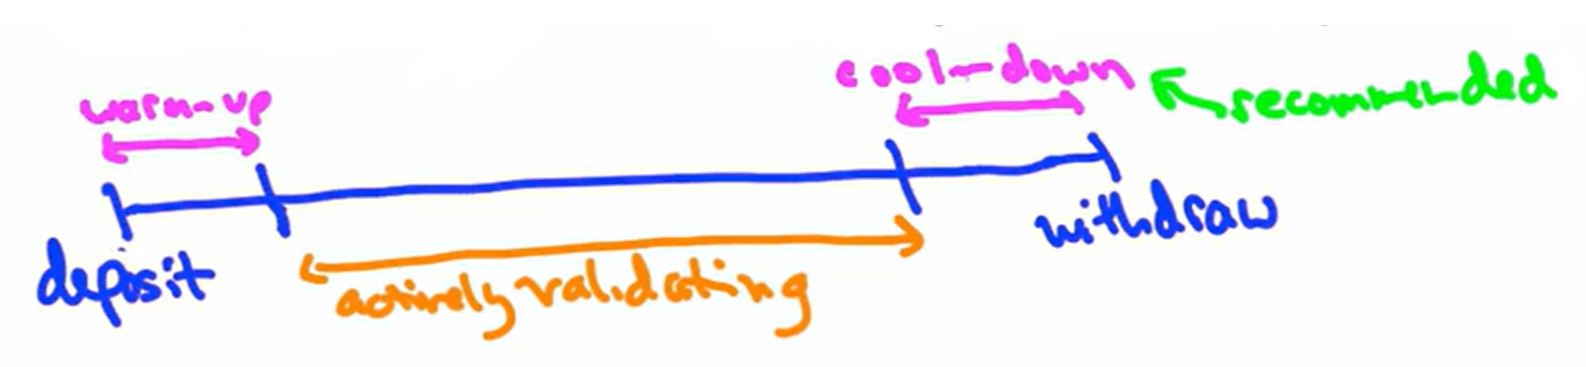
\includegraphics[scale = 0.5]{figures/f50.png}
    \caption{Warm-up and Cool-down Periods}
    \label{fig:mesh1}
\end{figure}\\

During the warm-up period, the node that has locked up its funds is not yet allowed to participate in the validation process. It is akin to a waiting period before the node gains the privileges of a validator. The warm-up period is essential for several reasons. First, it helps prevent immediate malicious behavior by delaying the node's ability to participate in validation. Second, it gives the network time to gather evidence of any potential misbehavior by the validator.\\
After the warm-up period, the node enters the active validation phase, where it can actively propose blocks, vote on other nodes' proposals, and contribute to the consensus process.\\
Once the node decides to withdraw its staked funds, it enters the cool-down period. During this period, the node is no longer allowed to participate in the validation process. However, the funds remain locked in the staking contract. The cool-down period is another essential feature for detecting and penalizing misbehavior. If the node engages in malicious actions, the network has time to gather evidence during the cool-down period and apply slashing mechanisms if necessary.

\subsection{Sampling Active Validators}
Once the staking mechanics are defined, we need to sample active validators from the list of public keys and their associated stake amounts. This sampling is critical for achieving Sybil resistance in the network. Simply selecting validators uniformly or randomly would be susceptible to Sybil attacks. Instead, validators are sampled with probability proportional to their stake amounts to ensure a fair and secure selection process.

\subsubsection{Challenges in Sampling}
Sampling active validators with probability proportional to their stake amounts is not a trivial task. Uniform or random selection could lead to vulnerabilities where a single malicious entity could control multiple validator slots by creating Sybil identities. To understand this, let's delve into the implications of random sampling.
Imagine a blockchain protocol with a list of public keys and associated stake amounts:


% \text{Public Keys: } \text{pk_1, pk2, ..., pk_n} 
% \par

% \text{Stake Amounts: } \text{q_1, q_2, ..., q_n} 
% \par
  Public Keys:  pk_1, pk_2, ..., pk_n

  Stake Amounts:  q_1, q_2, ..., q_n
 
If we randomly select validators to participate in consensus, each validator would have an equal chance of being selected, regardless of their stake amount. This means that an attacker with substantial resources could create numerous Sybil identities with small stakes, increasing their probability of being selected as validators.

\subsubsection{Importance of Sampling Proportional to Stakes}

To counteract the vulnerabilities of random selection, validators are sampled with probability proportional to their stake amounts. In this approach, the higher the stake a validator has, the more likely they are to be chosen for validation. This design aligns with the principle of Proof-of-Stake, as validators with more "skin in the game" have a greater incentive to act honestly and maintain the network's security.

For example, suppose we have three validators with the following stake amounts:

$$
\text{Validator 1: } \text{Stake = 100 coins}
$$
$$
\text{Validator 2: } \text{Stake = 50 coins}
$$
$$
\text{Validator 3: } \text{Stake = 200 coins}
$$

If we sample validators with probability proportional to their stakes, the chances of each validator being selected would be as follows:

$$
\text{Probability of selecting Validator 1} \propto 100
$$
$$
\text{Probability of selecting Validator 2} \propto 50
$$
$$
\text{Probability of selecting Validator 3} \propto 200
$$

Therefore, Validator 3 has the highest probability of being selected, followed by Validator 1 and then Validator 2.

\subsubsection{Achieving Sybil Resistance}
Sampling validators with probability proportional to their stake amounts ensures Sybil resistance in the network. Sybil resistance refers to the protocol's ability to resist Sybil attacks, where an adversary creates multiple identities to control the network's decision-making process.\\
By giving validators with more stake a higher chance of being selected, the protocol incentivizes honest behavior and discourages malicious actors from attempting to control the network. This system creates a more secure and robust blockchain protocol.\\
Sampling active validators with probability proportional to their stake amounts is a crucial aspect of designing a secure Proof-of-Stake blockchain protocol. This approach ensures that validators with significant economic commitments have a higher probability of participating in the consensus process, promoting network security and Sybil resistance against potential attacks. By carefully considering the design decisions related to staking mechanics and validator selection, a robust and resilient blockchain protocol can be created.

\section{Why Proof-of-Stake Is Hard}
The goal of Proof-of-Stake random sampling is to select a validator from a list of active validators with a probability proportional to their stake. The list of active validators is available in a designated staking contract. The selection probability ensures Sybil resistance, meaning the probability of a node being selected is independent of the number of identities, it uses.
\subsection{Sampling Procedure}
The sampling procedure in Proof-of-Stake (PoS) random sampling is a crucial aspect of consensus protocols. Its main objective is to select a validator from a list of active validators in such a way that the selection probability is directly proportional to the validator's stake. To better understand this process, let's break it down step by step based on the explanation given in the transcript:

\begin{itemize}[label=--]
\item \textbf{Input:} The initial input for the PoS random sampling is a list of active validators. These validators are the participants who are currently taking part in the consensus process. Each validator is identified by its public key, which serves as its unique identifier in the system.

\item \textbf{Stake-Associated Validators:} Each validator in the list is associated with some amount of stake. The term "stake" refers to the financial value or collateral that a validator commits as part of their involvement in the consensus protocol. This list of active validators and their corresponding stakes is available in a designated staking contract. This contract manages and maintains the state of the staking process.

\item \textbf{Probability Proportional to Stake:} The key objective of the sampling procedure is to select a validator at random, but with a probability directly proportional to their stake in the network. For instance, consider a scenario where there are ten validators, and one validator owns one percent of the total stake locked up in the network. In this case, that particular validator should have a one percent chance of being selected in the random sampling process.

\item \textbf{Sybil Resistance:} Ensuring Sybil resistance is a fundamental reason for sampling validators based on their stake. Sybil resistance means that the probability of a validator being selected as a leader or block proposer is independent of the number of identities or public keys that validator holds. In other words, a validator's chance of being selected depends solely on the total amount of stake they possess, regardless of how many public keys they own or use.

\item \textbf{Bounding Adversarial Power:} By sampling validators based on their stake, the protocol limits the power of adversarial nodes. The assumption made for a BFT (Byzantine Fault Tolerance) type consensus protocol is that the total stake controlled by Byzantine nodes (potentially malicious nodes) should be less than one-third of the overall stake. Similarly, for a longest chain protocol, the assumption is that the stake controlled by Byzantine nodes should be less than half of the total stake.

\end{itemize}
The sampling procedure is crucial for maintaining the integrity and security of the consensus protocol. It ensures that validators are selected in a fair and unbiased manner, where their stake directly influences their likelihood of being chosen to propose a block or lead a round in the consensus process. This, in turn, contributes to the stability and robustness of the blockchain network.

\subsection{Using Random Sampling in Consensus Protocols}
Random sampling plays a crucial role in consensus protocols, where the goal is to achieve agreement among nodes on the state of the blockchain. Two common types of consensus protocols are the longest chain protocol and the BFT (Byzantine Fault Tolerance) protocol.
\begin{itemize}[label=--]
  \item Random sampling can be used to select a leader (block proposer) for a round in consensus protocols like longest chain or BFT (Byzantine Fault Tolerance).
  \item Longest chain consensus requires the assumption that less than half of the stake is controlled by Byzantine nodes.
  \item BFT consensus protocols require the assumption that less than one-third of the stake is controlled by Byzantine nodes.
\end{itemize}

\subsubsection{Longest Chain Consensus Protocol}
In the longest chain consensus protocol, the blockchain maintains a chain of blocks, and the protocol aims to extend this chain with new blocks. The validators, who are active participants in the consensus, propose and validate new blocks to be added to the chain. The protocol requires that the majority of validators agree on the next block to be added to the chain to ensure security and consistency.\\
To use random sampling in the longest chain protocol, a leader (block proposer) is selected for each round. The leader's responsibility is to propose the next block that will be added to the chain. Here, the random sampling procedure comes into play to determine which validator gets selected as the leader for a specific round.\\
Let's take an example to understand the process better. Suppose there are ten active validators in the network, each with a different amount of stake in the blockchain. Validator 1 has 5\% of the total stake, Validator 2 has 3\%, Validator 3 has 10\%, and so on, up to Validator 10 with 2\% stake. The sum of all stakes is equal to 100\%.\\
The random sampling procedure aims to select a validator to be the leader for the current round based on their stake percentage. For example, if Validator 3 has 10\% of the total stake, they will be selected with a probability of 10\%. Similarly, if Validator 7 has 1\% stake, they will have a 1\% chance of being chosen as the leader for the round.\\
This random selection process ensures that each validator has a probability of being selected as the leader proportional to their stake. Hence, validators with higher stakes are more likely to become leaders, reflecting their greater influence and responsibility in the consensus process.

\subsubsection{BFT (Byzantine Fault Tolerance) Consensus Protocol}

In the BFT consensus protocol, a round-based system is also used, and a single designated node acts as the leader for each round. The leader's role is to propose a block for the current round, and the other validators (non-leader nodes) vote on whether to accept the proposed block or not. The protocol requires a supermajority (e.g., more than 2/3 of the total stake) of validators to agree on a block for it to be considered valid.\\
Using random sampling in a BFT consensus protocol involves selecting the leader for each round and determining which active validators are allowed to vote on the proposed block. The random sampling procedure helps ensure fairness and Sybil resistance in the protocol.\\
For instance, if the total stake in the network is 100 tokens and Validator 5 holds 30 tokens, they will have a 30\% probability of being chosen as the leader for the current round. The remaining 70 tokens of the total stake will belong to other validators, each with its own probability of being selected.\\
Additionally, validators' voting power in the BFT protocol is typically weighted by their stake. For example, if Validator 8 has 15 tokens, they will have 15\% voting power in the protocol, which means their vote will carry more weight when deciding the validity of a proposed block.

\subsection{Challenges of Proof-of-Stake Random Sampling}
The primary goal of Proof-of-Stake random sampling is to select a validator from a list of active validators with a probability proportional to their stake. In this context, a validator is identified by its public key and is associated with a certain amount of stake. The list of active validators, along with their stakes, is available in a designated staking contract.\\
The sampling procedure must ensure that a validator is selected with a probability proportional to the amount of stake it holds (also referred to as Q subbies). For instance, if a validator owns one percent of the total locked-up stake, it should be chosen as a block proposer with a one percent probability. This property is crucial as it ensures Sybil resistance within the protocol.\\
Sybil resistance is a desirable characteristic that ensures the probability of a node being selected is independent of the number of identities it uses. In other words, whether a validator operates with a single public key or multiple public keys, its selection probability depends solely on the overall amount of stake it possesses. This prevents adversaries from creating multiple identities (Sybil attacks) to increase their chances of being selected as block proposers.\\
Furthermore, sampling validators with probability proportional to stake allows for clear assumptions about the power of potential adversaries. In BFT (Byzantine Fault Tolerance) type consensus protocols, it is assumed that less than one-third of the overall stake is controlled by Byzantine nodes. On the other hand, for longest chain protocols, the assumption is that less than half of the stake is controlled by Byzantine nodes. These assumptions help in bounding the influence of adversaries within the protocol.\\
Utilizing random sampling in consensus protocols involves selecting a leader or block proposer for a given round. Both longest chain consensus and BFT-type protocols, like Tendermint, have a notion of rounds, and each round begins with a designated node acting as the leader with a block proposal.\\
For permissionless consensus protocols, like longest chain, integrating Sybil-resistant random sampling becomes pivotal. It essentially reduces the problem of designing a permissionless consensus protocol to a problem already solved for permissioned consensus protocols. In essence, permissionless longest chain is just permissioned longest chain combined with Sybil-resistant random sampling to choose a leader for each round.\\
Similarly, BFT-type consensus protocols build on the permissioned version, leveraging the random sampling procedure to select a leader for each round. In BFT protocols, the selection of active validators allowed to vote on a block proposal is determined, and their votes are weighted by the amount of stake they hold. Achieving a supermajority in BFT protocols, meaning more than two-thirds of the overall stake voting to proceed with a specific block, is a key defining property of Proof-of-Stake. However, despite the apparent simplicity and well-defined distribution, the challenge of Proof-of-Stake random sampling is surprisingly tricky, especially within the context of a blockchain protocol.\\
One of the primary challenges lies in generating randomness from within the hermetically sealed environment of the blockchain protocol. In Proof-of-Work protocols, randomness is obtained for free through an external mining process, where miners repeatedly try nonces to find solutions to cryptographic puzzles. The first miner to find a valid solution effectively gets selected as the leader for that round, ensuring a fair selection process.\\
In contrast, Proof-of-Stake protocols lack a clear analog to this external mining process, leaving the protocol to generate randomness internally from the information available in its current state. This creates a novel challenge as the protocol's internal state becomes the source of randomness.\\
As a result, validators themselves, who are responsible for producing and finalizing blocks, can potentially manipulate the blockchain state to influence the randomness derived from it. This opens up the possibility of validators trying to increase their chances of being selected as leaders by manipulating the contents or metadata of a block proposal. This manipulation could lead to certain validators being selected more frequently than they would have been under a fair, unbiased sampling process.\\
Since the randomness is derived from the blockchain state, it becomes possible for validators (who control the blockchain state) to manipulate the randomness by making strategic decisions in block proposals. This manipulation can lead to biased leader selection and potentially compromise the fairness and security of the Proof-of-Stake protocol. In this sense, the possibility of validators manipulating the blockchain state to influence randomness is the "new attack vector" that arises in the Proof-of-Stake context, which was not present in the Proof-of-Work world.\\
While in principle, one could import randomness from an external source, the question of trust arises. Who would be allowed to inject randomness into the Proof-of-Stake protocol, and how can it be ensured that the submitted randomness is genuine and not manipulated? Most major deployed Proof-of-Stake protocols prefer to generate their randomness internally, making the challenges of internal randomness generation highly relevant to the current state of the art.

\section{Weighted Robin-Round}
This section is the start of Part Two of chapter 12, focusing on the challenges in the design of proof-of-stake (PoS) blockchain protocols. The main challenge is the need to randomly sample a public key from a list of active validators, each with corresponding stake amounts, with probability proportional to their stake.

\subsection{Generating Randomness in PoS Protocols}
In PoS protocols, generating randomness is a critical aspect since there is no external process like mining in Proof-of-Work (PoW) protocols to provide it. Generating randomness internally in PoS protocols becomes necessary, and this process introduces some challenges.\\
One of the main challenges in PoS protocols is randomly sampling a public key from a list of active validators, each with corresponding stake amounts, with probability proportional to their stake. This process is crucial for selecting leaders to propose blocks in the blockchain. The goal is to achieve a fair and unbiased selection, where validators with higher stakes have a higher probability of being chosen as leaders.\\
In PoS protocols, unless you are willing to trust some third party to supply randomness, there is no external source of randomness generation like mining in PoW. Therefore, PoS protocols must generate randomness internally, directly from the blockchain state. This internal generation opens up an attack vector, as block producers could potentially manipulate the blockchain state to influence randomness and consequently, the probability with which different public keys are selected as leaders.\\
To tackle this problem, we introduce a "quick and dirty" solution called "weighted round robin." The idea behind weighted round robin is to reframe the problem slightly. Instead of sampling one public key at a time, the protocol generates a batch of public keys (e.g., 10,000) in advance. These public keys are selected with a near proportional representation of the validators' stake amounts.\\

\subsection{Determining Leader Sequence}
In Proof-of-Stake (PoS) blockchain protocols, the process of determining the leader sequence is crucial for selecting validators to propose blocks in each round. The goal is to have a sequence of leaders with proportional representation of the active validators' stake amounts. This sequence can be achieved through the concept of weighted round robin.\\
We now introduce the notion of "epics," which are batches of rounds. The number of rounds in an epic is controlled by a parameter \(N\). For example, let's consider an epic with \(N = 10,000\).\\
To start an epic, the protocol needs to specify the leader sequence. Various approaches can be used to derive this sequence from the list of active validators and their stake amounts. One simple and deterministic method is illustrated with an example:\\
\ex{
Suppose there are three active validators: A, B, and C, with stake amounts 2, 1, and 2, respectively. The deterministic leader sequence would be as follows:
$$A, A, B, C, C$$
This sequence is created by selecting each validator a number of times proportional to their stake. Validator A, with a stake of 2, appears twice, while B and C, with stakes of 1 and 2, appear once and twice, respectively. If \(N\) is a multiple of five (as in this example), the representation will be perfectly proportional. For instance, with \(N = 50\), we would have 20 A's, 10 B's, and 20 C's.\\
However, if \(N\) is not a multiple of five, there might be slight deviations in the representation. For example, with \(N = 10,000\) and the given stake amounts, we may end up with slightly over 4,000 A's, slightly over 2,000 B's, and slightly over 4,000 C's.}

To further enhance the protocol's randomness, we can apply a pseudo-randomly defined permutation to the deterministic leader sequence while preserving its proportional representation. This way, we achieve a more randomized order of leaders within each epic.\\

In summary, the process of determining the leader sequence involves creating an epic with \(N\) rounds and ensuring that the sequence of leaders reflects the proportional representation of the validators' stake amounts. Various deterministic or randomized methods can be employed to derive this sequence, allowing for better coordination among honest validators and reducing predictability.

\subsection{Pros and Cons of Weighted Round Robin}
The weighted round robin solution for sampling in proof-of-stake (PoS) blockchain protocols has its merits and drawbacks. Let's explore them in detail:

\subsubsection{Pros:}
\noindent
\textbf{Simplicity and Ease of Implementation}
The weighted round robin approach is relatively simple to implement and debug. Unlike some other more sophisticated methods, it does not require the use of advanced cryptographic techniques. The simplicity of the solution makes it easy for developers to understand and incorporate into their PoS protocols.\\

\noindent
\textbf{Straightforward Explanation}
The concept of weighted round robin can be easily explained to all stakeholders involved in the blockchain network. The straightforward nature of the solution allows participants to understand how the leaders are selected in the protocol without delving into complex mathematical or cryptographic principles.\\

\noindent
\textbf{Representation of Stake Amounts}
The primary objective of the weighted round robin solution is to achieve near proportional representation of validators' stake amounts when selecting leaders for each round (or epic). The sequence of leaders is designed to reflect the distribution of stakes, ensuring that validators with more stake have a higher chance of being chosen as leaders, while validators with less stake have a proportionally lower probability.\\

\noindent
\textbf{Practical Application}
Despite its limitations, the weighted round robin approach has been successfully used in practice by some PoS blockchains. Notably, older PoS protocols from 2016 to 2018 have implemented this method. While more sophisticated techniques have emerged in recent years, the weighted round robin remains a reasonable starting point for those seeking a quick and dirty solution for leader selection in a PoS blockchain.\\

\noindent
\textbf{Deterministic and Shuffle-based Approaches}
The weighted round robin can be implemented using deterministic methods or enhanced with shuffle-based techniques to achieve better randomness while preserving proportional representation. For example, a simple deterministic leader sequence can be combined with a pseudo-random permutation to further improve the selection process while maintaining fairness.\\

\subsubsection{Cons:}
\noindent
\textbf{Predictability of Leaders}
The most significant drawback of the weighted round robin solution is that it reveals the identity of future leaders well in advance. In PoS protocols, an "epic" consists of a batch of rounds, and each epic's sequence of leaders is predetermined. This predictability is dependent on the choice of $N$ (the number of rounds in an epic) and the block creation frequency. The longer the epic, the more time participants have to know in advance who the leaders will be, which can lead to various security issues.\\

\noindent
\textbf{Manipulation by Bad Actors}
The advanced knowledge of future leaders allows bad actors to potentially manipulate the protocol for their benefit. For example, an attacker might attempt to disrupt the liveness of the blockchain by coercing or bribing future leaders to skip their turn or propose empty blocks. This can lead to a breakdown in the integrity of the blockchain and affect its normal operation.\\

\noindent
\textbf{Security Risks in Fully Permissionless Protocols}
While predictability might be less concerning in semi-permissioned protocols with reputable validators, it becomes a significant issue in fully permissionless settings. In a fully open blockchain, validators might not have the resources or defenses to fend off serious denial-of-service (DoS) attacks or other forms of manipulation. This makes the predictability of leaders a more critical concern.\\

\noindent
\textbf{Need for Better Solutions}
Given the limitations and risks associated with weighted round robin, there is a growing demand for more sophisticated and secure methods for proof-of-stake sampling. Solutions like randomness beacons and verifiable random functions are being explored to address the predictability problem and improve the selection of leaders in a PoS blockchain without revealing them in advance.

\subsection{Perils of Predictable Leaders}
The predictability of leaders in a proof-of-stake (PoS) blockchain protocol poses several risks that may undermine the system's security and integrity. In the weighted round robin solution, where batches of leaders are selected well in advance, everyone knows who the leaders will be before they actually propose blocks. This predictability can lead to various malicious activities that could harm the protocol.

\subsubsection{Threats to Blockchain Liveness}
One major concern with predictable leaders is that bad actors may exploit this advanced knowledge to disrupt the liveness of the blockchain. For instance, an adversary could aim to prevent any valid blocks from being added to the blockchain during their turn as a leader. While normally a bounded adversary, controlling less than a third of the blocks, wouldn't significantly impact liveness, knowing the future leaders in advance changes the situation.\\
Even if the adversary controls no nodes themselves, they could still identify future block proposers and take actions to hinder them during their turn. This may involve coercion, bribery, or launching denial-of-service (DoS) attacks to prevent the leader from connecting to the network during their round. As a result, the adversarial influence could be greater than expected, potentially causing serious disruptions to the protocol's operation.

\subsubsection{Benefit to Honest Validators}
On the other hand, some blockchain protocols may view the predictability of leaders as a beneficial feature. Honest validators can use this information to optimize their operations and coordinate more efficiently. For instance, if a validator knows it won't be the leader in the next round but has information on pending transactions, it can forward those transactions directly to the next leader, avoiding broadcasting them to the entire network. This behavior may reduce redundant message propagation and improve the overall efficiency of the protocol.

\subsubsection{Considerations in Semi-Permissioned Protocols}
In certain scenarios, particularly semi-permissioned blockchain protocols, the drawbacks of predictability might not be as concerning. In semi-permissioned setups, validators are typically well-known and reputable entities with significant resources at their disposal. They might have robust defenses against DoS attacks and be less susceptible to coercion or bribery.\\
Since the validators' reputations are at stake, they are more likely to act honestly and in the best interest of the protocol. Consequently, predictability might not be as much of a risk in such cases, and the weighted round robin approach could be a viable and straightforward solution.

\subsubsection{Challenges in Fully Permissionless Protocols}
However, in fully permissionless protocols, where validators are anonymous and resources vary widely, predictability can become a serious concern. Validators with limited resources may struggle to defend against sophisticated DoS attacks, making them more vulnerable to coercion or manipulation by bad actors. In such settings, the predictable leader selection mechanism could enable adversaries to exert significant control over the protocol, leading to undesirable outcomes.

\subsection{Next Steps}
We now move forward to explore more sophisticated solutions to address the predictability issues associated with weighted round robin and enable better proof-of-stake (PoS) sampling.

\subsubsection{The Need for Improved Sampling}
While the weighted round robin solution has some practical applications, it falls short in fully permissionless PoS protocols. In such cases, it becomes crucial to avoid revealing the identity of future leaders well in advance, as this could lead to various manipulation and attack scenarios.

\subsubsection{Exploring Randomness Beacons}
One potential avenue for achieving better PoS sampling is through the use of randomness beacons. A randomness beacon is a source of unpredictable and unbiased random values that can be used in the blockchain protocol to select leaders. Unlike traditional sources of randomness, such as external mining processes in proof-of-work protocols, randomness beacons provide internal and trustworthy randomness generation.

\subsubsection{Leveraging Verifiable Random Functions (VRFs)}
Another promising solution is to incorporate verifiable random functions (VRFs) into the PoS protocol. A VRF allows a party to generate a random output that can be publicly verified to have been derived from a specific input value. By using VRFs, the blockchain can achieve a transparent and verifiable random sampling process.

\subsubsection{Benefits of Improved Sampling}
Utilizing randomness beacons or VRFs in PoS sampling offers several advantages:
\begin{itemize}
\item Leaders' identities remain unknown until the moment they are required to propose a block. This significantly reduces the window of opportunity for bad actors to manipulate the protocol.
\item The protocol's liveness and integrity are strengthened, ensuring that block production proceeds smoothly without undue influence.
\item Validators can participate without concerns about coercion, bribery, or denial of service attacks, as the element of surprise in leader selection helps maintain fairness and security.
\end{itemize}

\subsubsection{Potential Challenges}
While randomness beacons and VRFs offer promising solutions, implementing them effectively in a decentralized and secure manner can pose challenges. Ensuring the availability and reliability of randomness beacons, as well as properly designing and deploying VRFs, will be critical to the success of these approaches.


\section{Randomness Beacon}
In this section, we continue exploring approaches to Proof-of-Stake random sampling. The problem involves selecting a random validator from a list of active validators based on their associated stake amounts. The goal is to achieve proportional selection probabilities according to the stake distribution.

\subsection{Quick and Dirty Solution}
In the previous section, we discussed a quick and dirty solution to the problem. The main idea was to batch the selection process and schedule 10,000 leaders at a time, instead of choosing a single random sample. Let's delve into the details of this approach.

\subsubsection{Batched Selection}
To implement the quick and dirty solution, we schedule leaders in batches. Each batch consists of 10,000 leaders, and for each batch, we make sure that the public keys are represented proportionally to their staking amounts. This means that the more stake a validator has, the higher the chance they will be included in the batch.

\subsubsection{Relaxed Version of the Problem}
It's important to note that this approach solves a relaxed version of the original problem. Instead of selecting a single random sample from the public keys in the list, we are scheduling batches of 10,000 leaders at a time. Therefore, we never explicitly show how to pick just one random sample from the list of public keys.

\subsubsection{Drawbacks of the Quick and Dirty Solution}
While the quick and dirty solution provides a way to represent the public keys proportionally to their stakes, it has some significant drawbacks. One major issue is predictability.

\subsubsection{Predictability Issue}
With the batched approach, we determine the leaders for a batch well in advance. This predictability poses a security risk. Bad actors might exploit this knowledge to their advantage. For example, they could attempt to bribe or coerce validators who are scheduled to be leaders. Additionally, they could launch denial-of-service attacks on selected leaders, causing disruptions to the network.

\subsection{Improved Solution with a Randomness Beacon}
To address the predictability issue introduced by the quick and dirty solution, we aim to implement a stronger approach that samples public keys on a need-to-know basis. This improved solution relies on an ideal Randomness Beacon, which periodically emits perfect randomness visible to everyone.

\subsubsection{Ideal Randomness Beacon}
The ideal Randomness Beacon is conceptualized as a box that periodically emits uniformly random outputs, such as a 256-bit string. Each output is equally likely to be any of the $2^{256}$ possible 256-bit strings. Furthermore, this randomness is considered as a common knowledge, similar to a plane flying by in the sky with a 256-bit number trailing behind it, visible to all observers.

\subsubsection{Sampling Procedure}
Assuming access to the ideal Randomness Beacon, we can outline the steps of the Proof-of-Stake random sampling procedure:

\begin{enumerate}[label=(\alph*)]
  \item At a specific time $T$, the ideal Randomness Beacon emits a uniformly random output $r_t$.
  \item To interpret $r_t$ as a real number between 0 and 1, its 256-bit value is divided by $2^{256}$.
  \item The interval $[0, 1]$ is then partitioned into sub-intervals corresponding to the public keys of active validators. The lengths of these sub-intervals are proportionate to the stakes of the validators, and we denote the total stake across all active validators as $Q$.
  \item The random sampling procedure determines the public key corresponding to the sub-interval where $r_t$ falls.
\end{enumerate}

\subsubsection{Example}
Let's illustrate the process with an example. Suppose the ideal Randomness Beacon emits the value $r_t = 1011010010111\dots$ (a 256-bit string). We interpret this value as a real number between 0 and 1:

$$
\text{Real Number Value} = \frac{1011010010111\dots}{2^{256}}
$$

Suppose the total stake across all active validators is denoted as $Q = \sum_{j=1}^n q_j$. We divide the interval $[0, 1]$ into sub-intervals corresponding to the public keys of the validators, with lengths proportional to their stakes (Figure 12.2). For simplicity, let's consider three validators with stakes $q_1$, $q_2$, and $q_3$, where $Q = q_1 + q_2 + q_3$.

\begin{figure}[h]
    \centering
    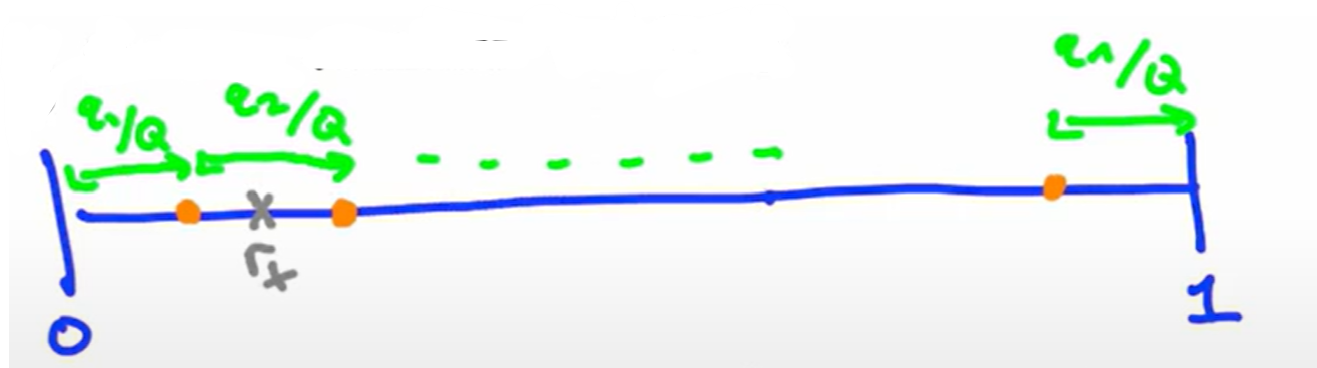
\includegraphics[scale = 0.5]{figures/f51.png}
    \caption{Mapping $q_i$s to [0,1] interval}
    \label{fig:mesh1}
\end{figure}\\
$$
\begin{array}{|c|c|}
\hline
\text{Public Key} & \text{Stake (q)} \\
\hline
pk_1 & q_1 \\
pk_2 & q_2 \\
pk_3 & q_3 \\
\hline
\end{array}
$$

The length of each sub-interval corresponding to the validators' public keys will be:

$$
\begin{aligned}
\text{Length of sub-interval for } pk_1 &= \frac{q_1}{Q} \\
\text{Length of sub-interval for } pk_2 &= \frac{q_2}{Q} \\
\text{Length of sub-interval for } pk_3 &= \frac{q_3}{Q} \\
\end{aligned}
$$

Depending on the real number value of $r_t$, it will fall into one of the sub-intervals, determining the selected public key and, thus, the chosen leader.
$$r_t \in \left[\frac{\sum_{j=1}^{i-1} q_j}{Q}, \frac{\sum_{j=1}^{i} q_j}{Q} \right]$$
\subsubsection{Selection Probabilities}
The key advantage of this sampling procedure is that the selection probabilities are directly proportional to the stakes of the validators. As $r_t$ is uniformly random between 0 and 1, the probability of it falling into a specific sub-interval is equal to the length of that sub-interval.

$$
\text{Probability of selecting } pk_1 = \frac{q_1}{Q}, \quad \text{Probability of selecting } pk_2 = \frac{q_2}{Q}, \quad \text{Probability of selecting } pk_3 = \frac{q_3}{Q}
$$
$$\Rightarrow \textbf{Pr}[\text{$pk_i$ selected}] = \frac{q_i}{Q}$$

This property aligns with the desired outcome of proportional selection probabilities based on the validators' stakes, as discussed in the previous section.


\subsection{Challenges and Next Steps}
\subsubsection{Secrecy of Leaders}
The current Proof-of-Stake random sampling procedure still suffers from a predictability issue similar to the weighted round-robin approach. When a leader is chosen, both the leader itself and anyone observing the network learn the identity of the leader simultaneously. This creates a small window of time during which bad actors could exploit the information for malicious purposes. For instance, bad actors could attempt to manipulate the block that the selected leader is assembling or launch a denial-of-service attack to prevent the leader from broadcasting any block at all.\\
In a practical scenario, even a small window of predictability, such as tens or hundreds of milliseconds, could be significant, as events on the internet can occur rapidly. Therefore, it becomes crucial to find a way to achieve secrecy in the Proof-of-Stake random sampling procedure. The goal is to ensure that only the selected leader knows their identity until they reveal it to the network. This secrecy property would prevent bad actors from gaining advanced knowledge of who the leader will be, thus mitigating their ability to carry out attacks based on this information.

\subsubsection{Approximating the Ideal Randomness Beacon}
The second major challenge lies in the assumption of having access to an ideal Randomness Beacon, which periodically emits perfect randomness visible to all participants. While the concept of an ideal Randomness Beacon is theoretically sound, its practical realization poses significant challenges. An ideal Randomness Beacon emits uniformly random outputs, such as 256-bit strings, with each output being equally likely to be any of the $2^{256}$ possible 256-bit strings.\\
In reality, obtaining such perfect randomness is nearly impossible, and therefore, the focus shifts to approximating the ideal Randomness Beacon using pseudo-randomness. Pseudo-randomness involves generating sequences of numbers that appear random but are actually produced by algorithms and can be replicated given the same starting conditions.\\
One potential approach to approximating the ideal Randomness Beacon involves the use of verifiable random functions (VRFs). VRFs are cryptographic tools that allow for the deterministic generation of random values based on a secret key and input data. These functions have the property that the randomness they produce can be publicly verified as authentic, ensuring that everyone in the network can agree on the same random value.\\
By incorporating VRFs into the Proof-of-Stake random sampling procedure, we can achieve the necessary randomness while still maintaining a level of verifiability that prevents bad actors from manipulating the system.

\section{Verifiable Random Functions (VRFs)}
In this section, we'll continue discussing approaches to Proof-of-Stake using random sampling. We have a list of public keys along with associated stake amounts, maintained by a designated staking contract. The goal is to randomly select one of those public keys from the contract with probability proportional to the stake amounts.\\
In the previous section, we saw a simple solution to this problem, but it had two significant issues. Firstly, it assumed access to an ideal Randomness Beacon, which is not practical in real deployments. Secondly, it lacked secrecy, as everyone found out the output of the sampling procedure at the same time.\\
In this section, we'll focus on addressing the second critique and explore more sophisticated ways of achieving random sampling with the additional secrecy property.

\subsection{Secrecy in Random Sampling}
In the previous section, we discussed the need for secrecy in the random sampling process in Proof-of-Stake protocols. The lack of secrecy in the initial solution raised concerns about potential attacks on the liveness of the consensus protocol. Here, we aim to address this issue by introducing Verifiable Random Functions (VRF).

\subsubsection{The Problem with Lack of Secrecy}
The lack of secrecy in the previous random sampling solution means that everyone finds out the output of the sampling procedure simultaneously. When a public key is selected, the owner becomes responsible for assembling a block and proposing it to others. However, they need some time to do this, and during this window of opportunity, attackers could launch a denial-of-service attack, effectively disrupting the consensus protocol's liveness.

\subsubsection{The Idea of Verifiable Random Functions (VRF)}
To tackle the secrecy problem, we turn to the concept of Verifiable Random Functions (VRF). VRFs are cryptographic primitives that allow a party with a private key to perform a computation that others cannot. This computation can be publicly verified using the corresponding public key. In our case, we want a computation that can only be performed by the owner of a public key, so that only they know if they have been selected.

\subsubsection{Using Digital Signature Schemes}
The key idea is to leverage digital signature schemes to achieve secrecy in the random sampling process. Each public key owner will sign the current Randomness ($r_t$) using their corresponding private key. Since only the owner of a private key can produce a valid signature (computing $\text{sig}_{sk_i} (r_t)$), this computation will remain secret to everyone else.

\subsubsection{Defining the Predicate for Selection}
To determine if a public key ($pk_i$) is selected at a given time step $t$, we define the predicate as follows:
$$
\text{PKI is selected at time t if } \text{Sig}_{sk_i}(r_t) < \text{Tau} \times \text{f}(q_i)
$$
Here, $\text{Sig}_{sk_i}(r_t)$ represents the signature of the current Randomness ($r_t$) using the private key $sk_i$ corresponding to $pk_i$. The value of $\text{Tau}$ is a difficulty threshold, similar to the one used in Proof-of-Work. The function $\text{f}(q_i)$ is an increasing function that depends on the stake amount ($q_i$) associated with $pk_i$.

\subsubsection{Secrecy and Verifiability}
The resulting inequality ensures secrecy in the random sampling process. Only the owner of a public key can compute the left-hand side, which involves generating the signature. Others can verify the signature using the public key ($pk_i$) and the Randomness ($r_t$). This verifiability ensures that the owner of a selected public key can easily prove their selection by broadcasting their signature.

\subsection{Manipulating the Probability of Selection}
To maintain the integrity of the protocol, we must ensure that public key owners cannot manipulate the probability of their selection. While the Randomness ($r_t$) is beyond manipulation as it comes from an ideal Randomness Beacon, any manipulation must involve the signature.\\
It is crucial to analyze the left-hand side of the inequality to prevent any potential manipulation. However, this issue will be revisited when we replace the ideal Randomness Beacon with a pseudorandom approximation in the next sections.

\subsection{VRF in Proof-of-Stake}
\subsubsection{The Grind Attack}
The Grind Attack is a potential concern when designing a Proof-of-Stake (PoS) protocol. It involves an attacker generating a massive database of public-private key pairs in advance. The attacker stores millions or even billions of key pairs, and this can be done by anyone without any special privileges or access.\\
When the Randomness $r_t$ is revealed, the attacker's goal is to find a private key from its precomputed database that, when used to sign the message $r_t$, produces a signature small enough to satisfy the sampling predicate. In other words, the attacker aims to find a private key such that the resulting signature is less than the threshold value, which determines whether a validator is selected or not.\\
For example, let's consider a hypothetical scenario. Suppose the threshold value for selecting validators is 0.5. The attacker has a large database of public-private key pairs and waits for the randomness $r_t$ to be revealed. Now, the attacker iterates through all the private keys it has and calculates the corresponding signature for the message $r_t$. If the attacker finds a private key that results in a signature less than 0.5, they have successfully "won the lottery" and can participate in the consensus as a validator.\\
This kind of attack is referred to as a "grind attack" because the attacker grinds through a large number of possible private keys, hoping to find one that satisfies the sampling predicate. It is analogous to the process of repeatedly trying different possibilities in the hope of winning a lottery.\\
The Grind Attack poses a significant threat to the fairness and security of a PoS protocol. If an attacker can manipulate the selection process by grinding through possible private keys, they could gain a disproportionate influence over the consensus and potentially control the network.\\
To counter the Grind Attack, the protocol must ensure that validators commit to their public-private key pairs before the randomness $r_t$ is revealed. This can be achieved through a warm-up period in the staking mechanics, where validators are required to deposit their stake and commit to their keys but are not yet allowed to participate in consensus (See Figure 12.3). By forcing validators to commit in advance, the protocol mitigates the risk of the Grind Attack, as the attackers cannot adjust their keys based on the revealed randomness.
\begin{figure}[h]
    \centering
    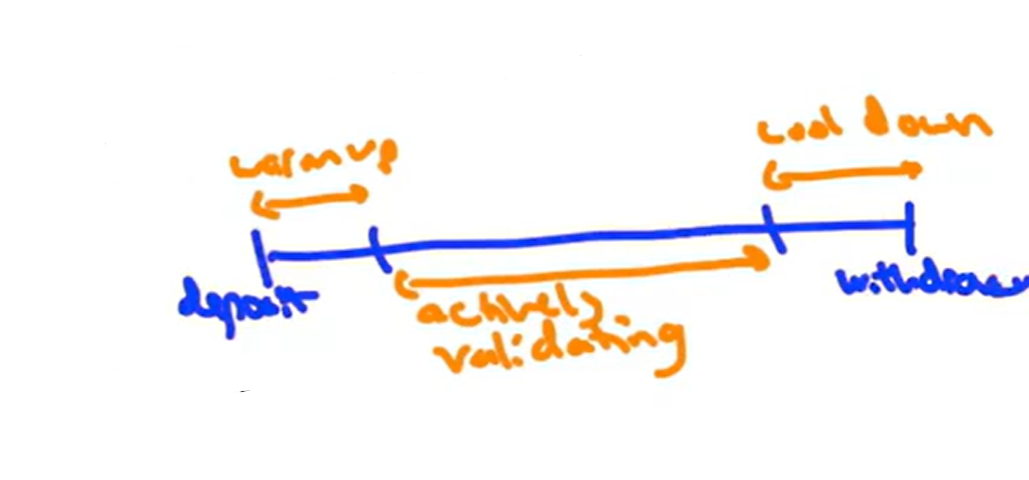
\includegraphics[scale = 0.5]{figures/f52.png}
    \caption{Fix for grind attacks}
    \label{fig:mesh1}
\end{figure}\\

\subsubsection{Unique Signatures and Fixing the Predicate}
In the context of Proof-of-Stake sampling, we encountered a potential issue with the uniqueness of signatures. Some signature schemes might have multiple valid signatures for the same message, which could allow an attacker to manipulate the sampling process. Let's delve into this issue and explore the solution using unique signatures and fixing the predicate.\\
Here, the concern is raised that an attacker could grind over all possible valid signatures for the message $r_t$ to try to find one that satisfies the sampling predicate. This "grind attack" could undermine the randomness and fairness of the protocol.\\
To address this issue, we require the signature scheme used in the Proof-of-Stake protocol to have the property of unique signatures. Unique signatures ensure that there is only one valid signature for a given message. BLS (Boneh-Lynn-Shacham) signature scheme is an example of a signature scheme that satisfies this property.\\
With unique signatures, the attacker is no longer able to manipulate the sampling process by grinding over different signatures. They are now restricted to one valid signature for the given message $r_t$.\\
The unique signatures fix the predicate by limiting the number of valid signatures for each message. This ensures that the left-hand side of the blue inequality, denoted as $Sig_{sk_i}(r_t)$, remains fixed for a particular validator, as they can only produce one valid signature for the given message $r_t$.\\
By fixing the predicate with unique signatures, we have made progress in achieving the secrecy and verifiability properties required for the Proof-of-Stake sampling process. Validators are forced to commit to their public-private key pairs in advance, and the attacker's ability to manipulate the left-hand side of the blue inequality is constrained.\\
However, it's important to note that not all signature schemes have unique signatures. For example, ECDSA (Elliptic Curve Digital Signature Algorithm), which is widely used in blockchain, does not have this property. Therefore, it is essential to select a signature scheme with unique signatures, such as BLS, when designing a Proof-of-Stake protocol to ensure the security and integrity of the random sampling process.

\subsection{Secrecy and Verifiability Properties of VRF}
Verifiable Random Functions (VRF) play a crucial role in achieving secrecy and verifiability in the random sampling process of Proof-of-Stake protocols. These properties ensure that the selection process remains secure and reliable.

\subsubsection{Secrecy Property}
The Secrecy Property of VRF ensures that a validator who knows their private key can efficiently compute the VRF and determine whether they have been selected for block production. This is analogous to how a participant who knows their private key can generate a digital signature on a given message.\\
Imagine a validator, "Alice," who possesses her corresponding private key $sk_i$. When the Randomness $r_t$ is revealed, Alice can quickly compute the VRF by applying the VRF algorithm with her private key and the current Randomness as inputs. The output will be a verifiable value based on her private key and the Randomness. Let's denote this VRF output as $VRF(sk_i, r_t)$.

\subsubsection{Verifiability Property}
The Verifiability Property of VRF allows anyone, who does not know the private key but has access to the corresponding public key $pk_i$, to efficiently verify the correctness of the VRF output. This is akin to how anyone can verify the validity of a digital signature using the corresponding public key.\\
For example, another participant, "Bob," who knows Alice's public key $pk_i$, can take the Randomness $r_t$ and the VRF output $VRF(sk_i, r_t)$ and verify that the VRF was indeed computed correctly by Alice. Bob can do this by applying the VRF verification algorithm using Alice's public key, the Randomness, and the VRF output as inputs.\\
This property ensures that the VRF output cannot be fabricated or manipulated by someone who does not know the private key. It allows other participants to independently confirm that Alice has been selected based on her VRF computation.

\subsubsection{Hard to Compute without Private Key}
The VRF is hard to compute without knowing the private key. This essential property is vital in ensuring that an attacker cannot forge VRF outputs and manipulate the selection process.\\
For example, if an attacker, "Eve," does not know Alice's private key $sk_i$, then Eve cannot compute $VRF(sk_i, r_t)$ on her own. The VRF algorithm is designed in a way that a polynomially bounded attacker, such as Eve, should not be able to derive the VRF output without the private key. This property helps maintain the integrity of the selection process.

\subsubsection{Hashing the VRF Output}
To enhance the appearance of randomness in the VRF output, we suggest passing the output through a cryptographic hash function. This process is called hashing the VRF output.\\
When the VRF output is passed through a cryptographic hash function, such as SHA-256, it becomes indistinguishable from a uniformly random value. This is a crucial step for certain analyses and ensures that the VRF output can be treated as a number between 0 and 1.\\
By incorporating all these properties, VRFs become a robust cryptographic primitive in Proof-of-Stake protocols. They offer a secure and efficient way for validators to compute and verify their selection status, ensuring the integrity and fairness of the consensus process.
By passing the VRF output through a cryptographic hash function, we can transform the fixed-size bit string into a value that seems to be uniformly random. This is important for various reasons:
\begin{enumerate}
    \item Uniform Distribution: The output of a cryptographic hash function behaves like a random function, distributing the hash values uniformly over the range of possible outputs. This allows us to treat the output as if it were a random number, making it suitable for various cryptographic operations.
    \item Pseudorandomness: Cryptographic hash functions exhibit pseudorandom properties, meaning the output appears indistinguishable from true random data to any efficient adversary. This property ensures that the hashed VRF output can be used securely in various cryptographic protocols.
    \item Security: Hashing the VRF output helps to hide the underlying VRF value, making it more difficult for potential attackers to reverse-engineer the original input.
    \item Consistency: Since the cryptographic hash function produces deterministic outputs for the same input, all participants can independently verify the hashed VRF output and achieve the same result, ensuring consistency in the verification process.
\end{enumerate}

Here's a summary of what we discussed:
\nt{
\noindent
\textbf{Issue \#1:} given $r_t$, try multiple pk-sk pairs\\
Fix: Use warm-up period($\tau$) must comit to $pk_i/sk_i$ pair before seeing $r_t$

\textbf{Issue \#2:} given $r_t + sk_i$, try multiple $\text{sig}_{sk_i} (r_t)$'s\\
Fix: Use DSS unique signatures(e.g BLS)

\textbf{Issue \#3:} $r_t$ uniform random \nRightarrow $\text{sig}_{sk_i} (r_t)$ uniformly random (in general)\\
Fix: Pass signature through a CHF + rely on a random oracle assumption}
\subsection{Challenges and Mitigations of VRFs}
While Verifiable Random Functions (VRF) offer significant benefits for achieving secrecy and verifiability in Proof-of-Stake protocols, there are still some challenges that need to be addressed:

\subsubsection{1. Selective Disclosure}
One challenge is selective disclosure of the VRF output. In some cases, validators may only want to reveal their selection status to specific parties or for specific purposes. However, VRFs inherently produce a verifiable output that can be publicly verified by anyone with the corresponding public key.\\

\noindent
\textbf{Mitigation:} To address selective disclosure, additional cryptographic techniques can be employed. For example, zero-knowledge proofs can be used to prove the validity of the VRF output without revealing the actual value. This allows validators to demonstrate their selection status without disclosing the VRF output to the public.

\subsubsection{2. VRF Output Uniqueness}
Ensuring the uniqueness of VRF outputs across different validators is crucial. If multiple validators produce the same VRF output for the same Randomness and message, it could lead to collisions and might disrupt the sampling process.\\

\noindent
\textbf{Mitigation:} Validators can add a unique identifier or nonce to the input of the VRF before computing the output. This ensures that even if multiple validators receive the same Randomness and message, their VRF outputs will differ due to the unique input, preventing collisions.

\subsubsection{3. Key Generation and Storage}
Key generation and secure key storage are essential to the security of VRFs. If an attacker gains access to a validator's private key, they can produce fraudulent VRF outputs and potentially manipulate the sampling process.\\

\noindent
\textbf{Mitigation:} Validators should use secure and robust key generation processes, such as using hardware security modules (HSMs) or secure multi-party computation (SMPC). Additionally, the private keys should be stored securely and protected against unauthorized access.

\subsubsection{4. Scalability}
As the number of validators in a Proof-of-Stake protocol grows, the scalability of VRF computation becomes a concern. Computing the VRF for each validator may become computationally expensive and slow down the overall consensus process.\\

\noindent
\textbf{Mitigation:} Optimizations can be implemented to improve VRF computation efficiency, such as parallelization and hardware acceleration. Additionally, using efficient and lightweight cryptographic algorithms can help reduce the computational overhead.\\

By leveraging VRFs with unique signatures, Proof-of-Stake protocols can achieve secure and private random sampling, enabling a robust and efficient decentralized consensus mechanism. As the blockchain space continues to evolve, VRFs and related cryptographic techniques will play a crucial role in ensuring the security and reliability of distributed systems.


\section{VRFs: Challenges and Mitigations}
In this section, we discuss the progress made towards achieving Proof-of-Stake random sampling with additional secrecy properties using Verifiable Random Functions (VRFs). VRFs are essential in ensuring that the sampling process is verifiable, secure, and efficient. We will also explore the challenges associated with the VRF-based approach and possible solutions.
At first, let's have a quick review of VRFs:
\begin{itemize}
  \item VRF is used for sampling public keys in the Proof-of-Stake mechanism.
  \item Each owner of a public key evaluates the VRF using their private key.
  \item Definition of a sampled public key: The VRF output with the corresponding private key is sufficiently close to zero.
  \item VRF properties:
  \begin{enumerate}
    \item Easy to evaluate with the appropriate private key.
    \item If someone knows the public key and the alleged VRF output with the private key, they can easily verify it.
    \item Secrecy property: No one can determine if a public key has been sampled unless the owner discloses it.
    \item Output is indistinguishable from uniform randomness when fed with random inputs.
  \end{enumerate}
\end{itemize}

\subsection{Challenges with VRF-Based Sampling}
The use of Verifiable Random Functions (VRFs) in Proof-of-Stake random sampling brings significant benefits in terms of verifiability and security. However, this approach also introduces several challenges that need to be addressed to ensure the efficiency and reliability of the sampling process.
\subsubsection{Variable Number of Samples}
The VRF-based sampling involves each owner of a public key independently evaluating the VRF using their private key. This evaluation process is akin to independent coin flips, where each public key owner may or may not be selected with some probability. This leads to two potential scenarios that must be dealt with:
\begin{enumerate}
    \item \textbf{Possibility of No Sampling:} There is a chance that none of the public keys' owners get sampled. This means that all the VRF outputs from the public key owners are not sufficiently small to meet the condition for sampling. In this case, no public key is selected as the leader for the current round. This situation can cause delays in the consensus process as no progress is made during the time slot.
    \item \textbf{Possibility of Multiple Samples:} On the other hand, it is also possible that two or more public keys' VRF outputs qualify as sufficiently small, resulting in multiple leaders for the current round. This situation deviates from the expected outcome of selecting exactly one public key from the pool.
\end{enumerate}
The ideal scenario is to have precisely one public key sampled in each round, as this simplifies the consensus process and ensures a smooth operation. However, due to the nature of independent coin flips through VRF evaluations, the number of samples obtained may vary.

\subsubsection{Options for Dealing with Challenges}
\noindent
\textbf{Option 1: Sacrificing Secrecy}\\
One way to address the challenges is to forego the secrecy property of the VRF-based sampling. By doing so, all the public key owners would find out the leader at the same time. This approach is simpler to implement but has its downsides.\\
For example, if the role of the leader is to assemble a block, then giving all the public key owners the leader information simultaneously creates a window of opportunity for attackers. During this window, anyone can launch a denial-of-service attack on the leader, causing the leader to skip its turn. This can hinder the progress of the consensus process and potentially introduce vulnerabilities.\\
Despite these drawbacks, some major blockchains, such as Solana and Cosmos, have chosen to adopt this approach and prioritize simplicity over the complexities of handling variable sampling.\\

\noindent
\textbf{Option 2: Adapting Consensus Protocols}\\
Other blockchain projects, like Algorand and Cardano, place a high value on the secrecy property and, therefore, employ the VRF-based sampling. However, doing so requires modifications to the consensus protocols to handle the possibility of multiple public keys being sampled in one round.\\
In traditional consensus protocols like BFD Tech consensus (e.g., Tendermint) or longest chain consensus, each round is expected to have a single unique leader. With VRF-based sampling, where multiple leaders can be selected, adjustments are needed to ensure the consensus protocol accommodates this quirk.\\
Handling the case where multiple leaders are sampled within one round is particularly tricky. It requires careful consideration and specific adaptations to the consensus mechanism to maintain integrity, consistency, and progress.\\

\noindent
\textbf{Option 3: Single Secret Leader Election (SSLE)}
The most ambitious approach is to aim for both secrecy and guaranteeing exactly one public key sampled in each round. This problem is known as Single Secret Leader Election (SSLE). The SSLE problem was formally defined in a 2020 paper by Bonet, Escandarian, Hanslik, and Greco.\\
While solutions to the SSLE problem exist in theory, practical implementations have not been deployed as of early 2023. The practicality and effectiveness of these solutions are still open questions. The SSLE approach represents the cutting edge of proof-of-stake blockchain design, and it is expected to be a focus in the next generation of blockchain protocols.

\subsection{Step 1: "Sufficiently Small"}
The concept of "sufficiently small" is crucial in the Proof-of-Stake random sampling process using Verifiable Random Functions (VRFs). It determines whether a public key is considered sampled or not, based on the VRF output evaluated with the corresponding private key and the current randomness value.

\begin{itemize}
\item The sampling decision: A public key is considered sampled if and only if the VRF output (obtained by evaluating the VRF with the corresponding private key on the current day's randomness) is sufficiently close to zero.

\item Stake Dependency: In the context of Proof-of-Stake, we want the probability of a public key being sampled to be proportional to the amount of stake associated with that public key. Hence, the right-hand side of the inequality used for sampling must be dependent on the stake associated with the public key.

\item function $f$: To ensure that public keys with higher stakes are sampled more frequently, we need to introduce a function $f$ that scales the right-hand side of the inequality with the amount of stake $Q$ associated with the public key. We can consider $f$ to be the identity function (first-order approximation), meaning the right-hand side scales linearly with Q. However, this simple scaling is not sufficient to ensure Sybil resistance.

\item Sybil Resistance: Sybil resistance refers to preventing an entity from manipulating the sampling probabilities by spreading its stake over multiple identities. To achieve Sybil resistance, the function $f$ needs to be carefully chosen to prevent such manipulations.

\item Choosing function $f$: The choice of $f$ is dictated by Sybil resistance requirements. In other words, $f$ should be designed to resist manipulation attempts while ensuring that public keys with higher stakes have a higher probability of being sampled.

\item Open Question: There are in principle solutions to the single secret leader election (SSLE) problem, the exact practical implementation of function $f$ remains an open question. This aspect is on the cutting edge of proof-of-stake blockchain design and is an active area of research.
\end{itemize}

\subsection{Simplified Scenario}
In the simplified scenario, we consider a case where all stake amounts, denoted by $q_i$, are integers. This simplification allows us to focus on the smallest possible stake amount, which is $q_i = 1$. This assumption implies that the stake is denominated in the smallest possible unit of the native currency used in the blockchain. For instance, in the case of Bitcoin, the smallest possible fraction of a Bitcoin is known as a Satoshi.\\
With the assumption that $q_i = 1$, the primary concern is to determine the value of the function $f$ at a single point, specifically when evaluated at $f(1)$. Without loss of generality, we can set $f(1)$ to be equal to $1$, which is merely a normalization step.\\
In this simplified scenario, we are interested in the probability of a uniformly random number between 0 and 1 (representing the VRF output) being less than a certain threshold $\tau$. The right-hand side of the blue inequality now becomes $\tau$, which is the difficulty threshold for the sampling process.\\
The probability that the VRF output is less than $\tau$ is equal to $\tau$ itself. For example, if $\tau$ is set to $1/100$, then the probability of a uniformly random number between 0 and 1 being less than $\tau$ is $1\%$. In other words, it will be less than $\tau$ approximately $1\%$ of the time and more than that the rest of the time.\\
Thus, the crucial decision in this simplified scenario is to determine the appropriate value for $\tau$. This parameter $\tau$ represents the probability that any given public key (which, in this case, has the minimum possible stake amount of 1) will be sampled.\\
The choice of $\tau$ depends on various factors, including the total stake amount and the number of public keys registered in the contract. For instance, if there are 100 public keys in the contract, all with a stake amount of 1, then a reasonable choice for $\tau$ could be $1/100$. This means that each public key has a $1\%$ chance of being sampled, and with 100 public keys in total, it leads to an expected value of one public key being sampled.\\
Similarly, if there are 1,000 public keys in the contract, each with a stake amount of 1, then a suitable choice for $\tau$ might be $1/1000$. This results in an expected value of one public key being sampled.\\
As a starting point, a natural choice for $\tau$ can be set to $1$ over the total stake amount (denoted as $\text{capital }Q$), targeting an expectation of one sample. This simplistic approach might be sufficient, but it could be further refined by adjusting $\tau$ using a multiplication or division factor to balance the frequency of different cases, such as having no one sampled versus having more than one person sampled.

\subsubsection{Generalizing to Arbitrary Stake Amounts}
Generalizing to arbitrary stake amounts involves addressing the issue of Sybil resistance, where an entity might try to manipulate the sampling probabilities by spreading its stake over multiple identities. Let's explore this process:\\
In the simplified scenario, we assumed that all stake amounts, $q_i$, are integers, and the smallest possible stake amount is $q_i = 1$. We also set the right-hand side of the inequality to $\tau$, the difficulty threshold, and interpreted the VRF output as a uniformly random number between 0 and 1.\\
Now, in the general case, we need to handle arbitrary $q_i$ values. To achieve Sybil resistance, we want to ensure that an entity is treated the same way, whether they stake a large amount under one public key or spread their stake across multiple public keys. In essence, we want to treat someone with, for example, 12 coins, exactly the same way, whether they register one public key with 12 coins or 12 public keys with one coin each.\\
The clever bit to achieve this is to treat a public key with a higher stake amount as if it were multiple public keys with smaller stake amounts. In this way, we can reduce the general case of arbitrary stake amounts to the previously solved simplified scenario where all $q_i$ are equal to 1.\\
For example, let's consider an entity that owns 12 coins and is contemplating representing themselves in the staking contract. They have two options:\\
\noindent
1-Stake all 12 coins under a single public key.\\
\noindent
2-Use multiple public keys and stake, for instance, 7 coins under one key and 5 coins under another.\\

To achieve Sybil resistance, we need to ensure that the probabilities of sampling the public key(s) in both scenarios are the same.\\
In the second scenario, the entity would prefer two or more of its symbols (public keys) to be sampled, as it cares about the exact number of sybils (public keys) getting selected.\\
To make both scenarios equivalent, we need to sample the public keys with multiplicities, meaning that they can be sampled multiple times based on a probability distribution.\\
The probability distribution for the multiplicities is given by the binomial distribution with parameters $Q$ (total stake amount) and $\tau$ (probability of sampling a public key with 1 coin). The binomial distribution represents the number of successes (sampled public keys) in $Q$ independent coin flips, where each flip has a probability of success $\tau$.\\
By using the binomial distribution to sample the public keys with multiplicities, we ensure that an entity's stake is treated the same way, regardless of how it is split across multiple accounts or public keys. This process ensures Sybil resistance and maintains the fairness and randomness of the sampling process in a proof-of-stake protocol.

\subsection{Step Two: Treating Higher Stake Amounts as Multiple Entities}
Here, we aim to address the issue of Sybil resistance, which arises when an entity can manipulate the sampling probabilities by spreading its stake over multiple identities. To achieve Sybil resistance, we need to treat someone with a higher stake amount as if they were multiple entities with smaller stake amounts. Let's dive into the details of this step:\\

For example, let's assume that there is a public key with 12 coins associated with it. One option available to the owner of these 12 coins is to launch a Sybil attack. In a Sybil attack, the owner could generate 11 more public-private key pairs and register them under different public keys, each with one coin. This would create 12 different identities, each holding one coin.

Now, to ensure Sybil resistance, we need to treat the owner of the 12 coins exactly the same, whether they register with a single public key holding 12 coins or with 12 public keys, each holding one coin. To achieve this, we reduce the general case of arbitrary stake amounts ($q_i$) to the seemingly trivial case where all $q_i$ are equal to one.

For instance, if we have three public keys with stake amounts of 12 coins, 7 coins, and 13 coins, respectively, we treat the first person as if they are 12 sybils with one coin each, the second person as if they are 7 sybils with one coin each, and the third person as if they are 13 sybils with one coin each. In this way, we can consider that we are working with a set of 32 public keys, each holding one coin.

Next, we need to determine the probability of selecting each public key with one coin in this scenario.\\
To do this, we refer back to Step One, where we defined "sufficiently small" using the parameter $\tau$. The probability of sampling a public key with the minimum possible stake amount (stake amount equal to one) is given by $\tau$. We can think of this as performing independent coin flips, each with a probability of coming up heads (selected) equal to $\tau$.\\
Now, we generalize this concept to all stake amounts ($q_i$). For a public key with a stake amount of $q_i$, we perform $q_i$ independent coin flips, each with a probability of being selected equal to $\tau$. As a result, the sampling probability for this public key becomes $1 - (1 - \tau)^{q_i}$.\\
Let's denote the right-hand side of this inequality as $1 - e^{-q_i \mu}$, where $\mu$ is defined as the natural logarithm of $\frac{1}{1 - \tau}$. Here, $\mu$ serves as a scaling parameter for $\tau$, and when $\tau$ is small, $\mu$ is approximately equal to $\tau$.\\
Now, the inequality can be expressed as:

$$1 - e^{-q_i \mu} \geq \text{VRF output}.$$
The VRF output is a value generated by the Verifiable Random Function for each public key.\\
Importantly, this inequality ensures Sybil resistance, as it treats each stake amount ($q_i$) as if it were the minimum possible stake amount (stake amount equal to one). Therefore, it doesn't matter how someone spreads their stake over multiple accounts or the specific stake distribution; the random sampling process treats them equivalently.

\ex{Consider someone who owns 12 coins and is deciding whether to stake them all under a single public key or split them into two public keys, one with 7 coins and the other with 5 coins.\\
\\
Scenario 1 (Staking 12 coins in one public key):\\
In this scenario, the person stakes all 12 coins under a single public key. The probability of this public key being sampled is given by the right-hand side of the blue inequality: $1 - e^{-12\mu}$.\\
Here, $\mu$ is a parameter related to the probability of sampling a public key with the minimum possible stake amount ($\tau$). $\tau$ represents the probability that any given public key, which has the minimum possible stake amount (in this case, 1 coin), gets sampled. It's a function of the total stake in the contract, denoted by $Q$.\\
\\
Scenario 2 (Staking 7 coins and 5 coins in two public keys):\\
In this scenario, the person divides their stake into two public keys, one with 7 coins and the other with 5 coins. However, unlike in Scenario 1, the person now cares about exactly how many of their public keys get sampled.\\
The probability of at least one of the two public keys getting sampled can be calculated as follows:
$$1 - (\text{probability that both keys are not sampled})$$
Since the events of each public key getting sampled are independent, we can compute this as:
$$1 - (1 - e^{-7\mu}) \times (1 - e^{-5\mu})$$
This expression accounts for the possibility that either the public key with 7 coins or the public key with 5 coins (or both) gets sampled.\\
By using the binomial distribution, we ensure that the probability in Scenario 2 is equivalent to the probability in Scenario 1.\\
The binomial distribution, bin($Q, \tau$), models the number of successful outcomes (sampled public keys) in $Q$ independent coin flips, where each coin flip has a probability of success ($\tau$) of being sampled. Therefore, Scenario 1 (staking 12 coins in one public key) and Scenario 2 (staking 7 coins and 5 coins in two public keys) will have the same probability as long as $Q=12$ and $\tau$ is the same.}

This clever approach ensures Sybil resistance, meaning that the entity cannot gain an advantage by splitting their stake across multiple public keys. Regardless of whether they stake all their coins in one public key or divide them into several public keys, they will be treated equivalently in terms of their sampling probability.\\
By implementing Step Two, VRF-based proof-of-stake blockchain protocols can achieve a fair and robust random sampling process, making it difficult for malicious entities to manipulate the system for their benefit.

\section{Pseudorandomness Beacons}
In this section, we will discuss Proof-of-Stake random sampling in blockchain protocols. The main focus is to relax the assumption of having access to an ideal Randomness Beacon, which provides independent uniform randomness.

\subsection{Ideal Randomness Beacon}
The concept of an Ideal Randomness Beacon is a central element in blockchain protocols, particularly in the context of Proof-of-Stake mechanisms. This beacon serves as a crucial source of independent uniform randomness, which plays a pivotal role in ensuring the security and fairness of various processes within the blockchain.\\
The notion of an Ideal Randomness Beacon can be visualized as a source of perfect randomness, akin to random values falling from the sky. This beacon operates periodically, emitting random values at defined intervals, such as once every second or once every ten seconds. These emitted values are considered to be independent and uniformly distributed within a known set, often exemplified as the set of all possible 256-bit strings.\\
Mathematically, we can represent the ideal beacon's output at time $t$ as $r_t$. This randomness is leveraged in blockchain protocols for various purposes, such as the selection of a block proposer in a Proof-of-Stake mechanism. In the context of Proof-of-Stake, $\delta_{t-1}$ represents the beacon randomness from the previous time step $t-1$, and it is used to compute the current beacon output $r_t$.

$$r_t = \text{Beacon Function}(\delta_{t-1})$$

The value of $\delta_{t-1}$ is derived from the randomness at the previous step and contributes to the overall randomness of the system at time $t$. This sequential dependency ensures that the output randomness is not only independent but also influenced by previous randomness, enhancing the security and integrity of the beacon.\\
This ideal beacon's output, denoted as $r_t$, holds a significant purpose in blockchain protocols. Specifically, it is crucial for a Proof-of-Stake protocol that aims to sample a public key from a set of registered public keys within a staking contract. This sampling process is designed to be proportional to the stake held by each public key. Notably, this becomes essential in scenarios where the goal is to select a block proposer based on their stake in the system.\\
In section 12.7, the weighted round-robin method was introduced, which allowed for the selection of a block proposer without relying on the ideal Randomness Beacon. However, in subsequent discussions, it was highlighted that this approach lacked the desired level of secrecy. The revelation of the selected public key was instantaneous as soon as the randomness was provided, preventing any form of delayed notification.\\
To address this limitation, we introduced a more sophisticated approach utilizing verifiable random functions (VRFs). These functions share similarities with secure digital signature schemes and offer improved privacy and security. The ideal Randomness Beacon's output $r_t$ served as a critical input for evaluating the VRFs, determining the block proposer while ensuring a level of secrecy. \\
Despite the advantages of incorporating VRFs, a significant challenge remains: the availability of a reliable source of perfect randomness, the Ideal Randomness Beacon. While the ideal scenario assumes the existence of such a beacon, practical implementations require a concrete definition of the source of randomness, especially if the ideal beacon is non-existent.\\
We have the option of outsourcing the production of $r_t$ to a third party. However, this approach introduces trust-related issues, such as the reliability of the third party and the potential for biased randomness. For major blockchain protocols, this trust assumption is untenable, as it contradicts the decentralized and secure nature of the systems.\\
It's important to note that some blockchain protocols based on Nakamoto consensus, such as Proof-of-Work protocols, do export randomness from the outside to some extent. However, this does not involve trusting a third party but rather relies on cryptographic assumptions, such as the random Oracle assumption.\\
In contrast, Proof-of-Stake blockchain protocols face a unique challenge. They generate randomness from within their enclosed environment, relying solely on their internal information. This poses a fundamental challenge when trying to implement Proof-of-Stake random sampling while maintaining security, fairness, and decentralization.

\subsection{Pseudorandomness Beacon}
The concept of a Pseudorandomness Beacon serves as an alternative to the ideal Randomness Beacon, allowing blockchain protocols to achieve the necessary randomness without relying on a perfect external source. The goal is to approximate the properties of an ideal Randomness Beacon while addressing the challenges of predictability and manipulability.

\subsubsection{Challenges of Perfect Randomness}
As discussed earlier, the assumption of having access to an ideal Randomness Beacon, which emits independent uniform randomness from a known set, is unrealistic. In practice, such a perfect source of randomness is unattainable. Outsourcing the task to a third party introduces trust issues, which is a concern, particularly for major blockchain protocols.

\subsubsection{Approach of a Pseudorandomness Beacon}
To overcome these challenges, a pseudorandomness beacon is proposed. This beacon aims to generate randomness within the protocol's internal environment, reducing reliance on external sources. The pseudorandomness is achieved through the use of cryptographic hash functions and carefully chosen inputs.

\subsubsection{Initial Attempt: Hashing the Time Step}
An initial approach is to simply hash the current time step to generate the pseudorandomness. However, this approach quickly reveals its flaws. Since the blockchain protocol knows the time step at deployment, all future pseudorandom seeds become entirely predictable. This predictability undermines the security and fairness of the protocol, making it unsuitable for practical use.

\subsubsection{Improved Approach: Incorporating Blockchain State}
To enhance the unpredictability of the pseudorandomness, a more sophisticated approach is adopted. The pseudorandomness beacon's input is constructed by concatenating the current time step with information derived from the blockchain state at that particular time. This approach introduces a level of complexity and variability that makes the pseudorandom seed less predictable.

\subsubsection{Function $f$ and Manipulation}
The choice of function $f$, which extracts information from the blockchain state, is crucial to minimizing manipulability. A key insight is to avoid direct dependency on the transactions within the blockchain. Instead, the function should rely on a factor that is less easily manipulated by individual nodes.

\subsubsection{Using VRF Outputs for Pseudorandomness}
A promising choice for $f$ is to incorporate the output of a verifiable random function (VRF) used by the previous block proposer. In this approach, the pseudorandomness depends on the VRF's output, which is determined by the previous block proposer's actions and their use of a private key.

\subsubsection{Reduction of Manipulability}
By utilizing the VRF output as an input for the pseudorandomness beacon, the protocol effectively reduces the degrees of freedom for manipulation. Nodes cannot arbitrarily influence the pseudorandomness by altering transaction content or ordering. Instead, their influence is restricted to actions involving VRF outputs and private keys.

\subsubsection{Balancing Predictability and Security}
While the improved pseudorandomness beacon reduces predictability and manipulability, it's important to note that no solution can completely eliminate these concerns. The goal is to strike a balance between providing secure and sufficiently unpredictable pseudorandomness while acknowledging that certain degrees of predictability may persist due to the nature of blockchain protocols.

\subsubsection{Formulaic Representation of Pseudorandomness}
The pseudorandomness beacon's output can be mathematically represented as follows:
\[
\text{Pseudorandomness}_{t} = H(\text{Time}_{t} \, || \, f(\text{Blockchain State}_{t}))
\]
Where:
\begin{itemize}
  \item $\text{Pseudorandomness}_{t}$ is the pseudorandom output at time $t$.
  \item $H$ is the cryptographic hash function.
  \item $\text{Time}_{t}$ is the current time step.
  \item $f$ is the function extracting information from the blockchain state.
  \item $\text{Blockchain State}_{t}$ is the state of the blockchain at time $t$.
\end{itemize}
To further enhance unpredictability, the pseudorandomness beacon's input can incorporate $\delta_{t-1}$, representing the time between blocks. This introduces an additional element of randomness based on the time elapsed since the last block.


\subsubsection{Future Directions: Verifiable Delay Functions (VDFs)}
Looking ahead, more experimental techniques are being explored to achieve completely unmanipulable pseudorandomness. One such approach involves verifiable delay functions (VDFs), which offer enhanced security guarantees. This direction represents ongoing research and has the potential to become the best practice in future iterations of Proof-of-Stake blockchain protocols.


\section{Crowdsourcing a Randomness Beacon}
In this section, we explore various approaches to implementing an approximation of a Randomness Beacon. We discuss the limitations of previous attempts and introduce a new method based on Verifiable Delay Functions (VDFs). Our goal is to crowdsource randomness from the nodes running the protocol to achieve a higher level of security and trust.
\subsection{Previous Attempts}
Previously, we got acquainted with an approach that involved deriving randomness, denoted as $r_t$, from signatures obtained from recent block proposers. While this approach appeared promising, it still came with certain limitations that need to be addressed.

\subsubsection{XOR of Contributions}
One initial attempt involved the concept of an XOR (exclusive OR) operation applied to all the contributions from the participating nodes in the protocol. Each node would generate its own set of pseudorandom bits and submit them to the protocol. The protocol's role was then to perform an XOR operation on these individual contributions, resulting in the value of $r_t$.
For a better understanding, let's delve deeper into the XOR operation. Consider the scenario where there are multiple public keys registered in the staking contract, say 20 of them. An honest node, which owns one of these public keys (let's say the 17th key), is responsible for generating pseudorandom bits and reporting them to the protocol. Of course, the node would also sign its contribution to establish authenticity.\\
During a specific period within the round, the protocol accepts these contributions from various nodes. However, not all nodes might submit their proposals. For instance, out of the 20 registered public keys, only 17 might actually submit their signed randomness proposals. The protocol then proceeds to compute the XOR of these submitted contributions. In this example, it would XOR the 17 submitted values.\\
Mathematically, XOR is a bitwise operation that involves toggling individual bits based on their values. For example, When XOR-ing two strings bit by bit, if both input bits are 0, the output bit will be 0, if both input bits are 1, the output bit will be 0. If only one input bit is 1, the output bit will be 1.\\
The XOR operation continues across all bits of the strings. It can also be visualized as column-wise addition without carries, equivalent to modulo 2 addition. However, despite its initial appeal, this approach had a critical vulnerability. If an attacker, armed with substantial computational resources and a deep understanding of the network, managed to gather knowledge of all the other submitted randomness contributions before submitting their own, they could exploit the XOR operation. By strategically choosing their bits, the attacker could manipulate the final output to their advantage. This ability to manipulate the result gave rise to a concerning "last-mover advantage" scenario.\\
To illustrate, imagine the attacker has insights into the XOR of the other 16 contributions. They could then tailor their own contribution to cause specific toggles in the final XOR output. This manipulation could allow the attacker to potentially steer the result toward their desired outcome, undermining the protocol's intended randomness.\\
This susceptibility to manipulation posed a significant threat to the integrity of the randomness generation process. As a result, it became evident that this approach needed further refinement to eliminate the last-mover advantage and ensure a more robust and tamper-resistant generation of randomness.\\
In the next section, we will explore an alternative approach based on Verifiable Delay Functions (VDFs) that addresses these limitations and provides a more secure foundation for crowdsourcing randomness in the protocol.
\subsection{Verifiable Delay Functions (VDFs)}
Verifiable Delay Functions (VDFs) provide a novel approach to implementing randomness generation in a secure and tamper-resistant manner. This method introduces a two-phase protocol that overcomes the limitations of previous attempts.

\subsubsection{Commit-Reveal Approach}
The core idea behind VDFs is to separate the randomness generation process into two distinct phases: the commit phase and the reveal phase.\\

\noindent
\textbf{Phase 1: Commit Phase}\\
In the commit phase, each participating node generates a commitment to their randomness contribution. This commitment is formed by calculating a cryptographic hash of their proposed randomness. Notably, this commitment is based solely on their input and is independent of other nodes' choices. Let's denote this commitment as $h(r_i)$, where $r_i$ represents the randomness contributed by node $i$.\\
This commit phase ensures that each node commits to a specific randomness value before learning about the contributions of other nodes. This property eliminates any last-mover advantage that an attacker might exploit.\\

\noindent
\textbf{Phase 2: Reveal Phase}\\
The reveal phase comes after the commit phase. During this phase, each node publicly reveals their actual randomness contribution, denoted as $r_i$. Importantly, the protocol verifies that the revealed randomness matches the previously committed hash $h(r_i)$. This verification step ensures that nodes are honest in disclosing their true contributions.\\
The two-phase structure of commit and reveal ensures that nodes cannot manipulate their contributions based on knowledge of other nodes' choices. An attacker attempting to alter their randomness contribution during the reveal phase would be detected through the mismatch between the revealed value and the committed hash.

\subsubsection{Properties of VDFs}
The distinguishing feature of VDFs is their verifiable delay. Unlike previous attempts, where contributions were merely XORed together, VDFs introduce a computational delay that prevents rapid manipulation. This delay is achieved through the inherent computational complexity of the VDF evaluation process.

\subsubsection{Benefits of VDFs}
The integration of VDFs into the protocol offers several significant benefits:

\begin{itemize}
    \item \textbf{Elimination of Last-Mover Advantage:} The commit phase ensures that each node commits to its randomness contribution before gaining knowledge of other nodes' contributions. This eliminates the possibility of exploiting a last-mover advantage to manipulate the output.
    
    \item \textbf{Slowing Down Attackers:} VDFs introduce a time delay between the commit and reveal phases. This delay prevents attackers from rapidly generating and testing multiple possibilities for their randomness contribution. As a result, attackers are unable to efficiently explore different options.
    
    \item \textbf{Tamper Resistance:} The cryptographic verification of committed hashes in the reveal phase, guarantees the authenticity of randomness contributions. Attempting to alter contributions becomes detectable and ineffective.
\end{itemize}

\subsection{Optimizing Phase Lengths}
A key consideration in the VDF-based approach is the optimal length of the commit and reveal phases. As mentioned earlier, the commit phase is designed to prevent last-mover advantage and ensure that nodes commit to their contributions without knowledge of others' choices. On the other hand, the reveal phase verifies the authenticity of contributions and guards against tampering.\\
The duration of these phases plays a crucial role in balancing security and efficiency. In practice, the length of the commit phase should be sufficiently short to prevent long delays in the protocol's operation. However, it must also be long enough to thwart attackers from rapidly exploring different options.\\
Similarly, the reveal phase should be long enough to allow honest nodes to complete the verification process and reveal their contributions. At the same time, it should be short enough to ensure timely completion of the protocol.

\subsection{The Future of VDFs}
Verifiable Delay Functions (VDFs) hold significant promise for implementing secure randomness generation. While the idea of utilizing computational delays to prevent manipulation is a promising step, there is ongoing research into designing efficient and secure VDF constructions.\\
Researchers are exploring various cryptographic techniques to optimize VDF performance and ensure their robustness against potential attacks. As the field evolves, VDFs may become a cornerstone of secure protocols, providing tamper-resistant and unbiased randomness for a wide range of applications.\\

The incorporation of Verifiable Delay Functions (VDFs) into the randomness generation protocol offers a robust and secure approach. By utilizing the commit-reveal structure and leveraging the computational delay of VDFs, the protocol achieves a higher level of trust and security. This method ensures that randomness contributions are tamper-resistant and unbiased, making it a promising solution for crowdsourcing randomness in various applications.

\section{Verifiable Delay Functions (VDFs)}
In this section, we delve into the concept of Verifiable Delay Functions (VDFs), a cutting-edge topic in the field of blockchain protocols. We will explore the properties and potential applications of VDFs, as well as their integration into permissionless consensus protocols.\\

\noindent
\textbf{Background:} Recapping the previous section, we discussed the challenge of sampling a secret leader from a staking contract with proportional stake. Now, we turn our attention to VDFs and their role in enhancing blockchain protocols.

\subsection{Properties of Verifiable Delay Functions (VDFs)}
VDFs, or Verifiable Delay Functions, are a fundamental concept in blockchain protocols that provide a unique set of properties crucial for enhancing the security and efficiency of distributed systems. Let's delve into the three defining properties of VDFs outlined in this section:

\begin{enumerate}[label=\arabic*.]
    \item \textbf{Computation Time Invariance}: One of the central objectives of VDFs is to achieve computation time invariance. This means that the time it takes to evaluate a VDF should remain relatively constant, regardless of the amount of computational resources thrown at it. In other words, the evaluation time of the VDF, denoted by parameter $T$, should be consistent and not significantly influenced by the computational power used.\\
    This property is particularly important because it ensures that honest nodes can evaluate the VDF within a reasonable time frame, using a reasonable amount of computational resources. The goal is to prevent scenarios where attackers with substantial computational resources gain a disproportionate advantage in evaluating the VDF more quickly than honest nodes. This property is crucial for the integrity and fairness of the blockchain protocol.

    \item \textbf{Sequentiality and Parallelism Resistance}: VDFs are inherently sequential functions, which means that they resist parallelism. While honest nodes typically have access to a single machine, attackers might have the means to deploy multiple machines in parallel. If a VDF could be easily parallelized, attackers could exploit this to achieve a significant speedup over honest nodes, compromising the security of the protocol.\\
    This property aims to ensure that parallelism does not provide an advantage in evaluating the VDF. In the context of VDFs, parallelism refers to the ability to divide the computation into smaller tasks that can be executed simultaneously on different machines. By resisting parallelism, VDFs maintain a level playing field between honest nodes and attackers.

    \item \textbf{Efficient Verification}: Efficient verification is a key requirement for VDFs. It refers to the ability of third parties, including honest nodes, to verify the correctness of a VDF computation without needing to redo the entire computation from scratch. This property addresses the practicality of VDFs in real-world blockchain protocols.\\
    We can provide an analogy with Verifiable Random Functions (VRFs) to help illustrate the concept of efficient verification. In a VRF, the correct computation can be quickly verified if the public key and output are known. Similarly, In a VDF, a supporting certificate (denoted as $\Pi$) is generated as part of the computation process. This certificate serves as a succinct proof that the VDF was correctly evaluated. By including this certificate, VDFs enable others to efficiently verify the computation's correctness without the need for redundant computations.\\
\end{enumerate}
In summary, VDFs offer a powerful combination of properties: consistent computation time, resistance to parallelism, and efficient verification. These properties collectively contribute to the reliability, security, and fairness of blockchain protocols by providing a reliable source of randomness and consensus within the distributed system.

\subsection{Candidate VDF Constructions}
A potential candidate for a Verifiable Delay Function (VDF) is the iteration of a cryptographic hash function, such as SHA-256, applied multiple times sequentially. This concept aligns with the sequentiality property of VDFs. The idea is to repeatedly apply the hash function to an input value, building upon the previous result with each iteration. This process intuitively seems inherently sequential, making it a reasonable starting point for a VDF.

For instance, if we consider using SHA-256 as the hash function and apply it sequentially several times to a given input \(X\), we obtain a sequence of hash values:

\(\text{SHA-256}(X), \text{SHA-256}(\text{SHA-256}(X)), \text{SHA-256}(\text{SHA-256}(\text{SHA-256}(X))), \ldots\).

This straightforward approach to compute the VDF, however, does not fully meet the requirements of a VDF, specifically the efficient verifiability property. In a permissionless consensus protocol, where nodes can join and leave at any time, there's a need for efficient catching up with the blockchain's history. If VDF computations were integral to every block and required substantial time to validate, it would be impractical for new nodes to catch up with the chain.

Imagine a scenario where each block involves a lengthy computation of the form

\(\text{SHA-256}(\text{SHA-256}(\ldots(\text{SHA-256}(X))\ldots))\).

If a node were to join the network years later, it would need to redo the entire computation for all previous blocks, which would be computationally prohibitive and time-consuming. This issue contradicts the efficient verification property. To address this challenge, an important requirement arises: the ability to verify the correctness of VDF computations without having to redo the entire computation. This need leads us to consider more advanced constructions that offer efficient verification.

\subsection{Efficient Verification and Catching Up in Blockchain Protocols}
In the context of blockchain protocols, the concept of efficient verification plays a crucial role. Blockchain nodes need to be able to catch up with the blockchain's history without the burden of redoing all the computations. This requirement becomes particularly important in permissionless consensus protocols, where nodes may join the network at any time.\\
Consider the scenario where a new node joins a blockchain network that utilizes verifiable delay functions (VDFs) for generating randomness or making decisions. Let's use the example of a VDF-based blockchain protocol where each round involves the evaluation of a VDF to generate pseudorandomness for that round. This pseudorandomness is then used to determine various aspects of the protocol.\\
Now, imagine this newly joined node wants to participate in the blockchain's current round, but it needs to verify the correctness of the previous VDF evaluations to ensure the integrity of the pseudorandomness used in those rounds. Without efficient verification, this process could become impractical, especially if the VDF computation requires a significant amount of time and resources.\\
To put this into perspective, let's use the analogy of a Bitcoin or Ethereum node. If someone were to set up a new node today, they would need to synchronize with the entire blockchain's history to validate transactions and blocks. This process can be time-consuming and resource-intensive, especially if the blockchain's history spans several years. In the case of VDF-based protocols, where each round involves a VDF evaluation, efficient verification becomes essential to enable new nodes to catch up quickly without redoing all the computations.\\
The concept of efficient verification aligns with the third defining property of VDFs, which states that if someone has already computed the VDF and generated a corresponding certificate (Pi), other nodes should be able to verify the correctness of the computation without the need to redo the entire process. This property is crucial for scalability and the smooth operation of permissionless consensus protocols.\\
In the context of VDFs, efficient verification allows new nodes to quickly validate the pseudorandomness generated in previous rounds without having to recompute the entire VDF evaluation. This property ensures that the blockchain remains accessible to newcomers and maintains a level of efficiency that enables the network to grow and evolve over time.

\subsection{Verifiable Random Functions (VRFs) vs. Verifiable Delay Functions (VDFs)}
Both VRFs and VDFs exhibit properties that contribute to their effectiveness in different aspects of blockchain protocols.\\

\noindent
\textbf{1. Quick Evaluation:}
VRFs enable quick evaluation, where knowing the correct private key allows one to rapidly compute the function's output. Similarly, VDFs possess the property that an honest node can evaluate them in a reasonable amount of time using a reasonable amount of computation power. In both cases, the ability to quickly compute the function's output is a key feature.\\
The time spent on computation in VDFs is analogous to the private key's role in VRFs. This analogy suggests that in VDFs, the effort put into the computation (akin to having the private key) is what enables fast evaluation.\\

\noindent
\textbf{2. Uncertainty and Resistance to Attacks:}
VRFs provide unguessability, meaning that without knowing the private key, it is practically impossible to predict the function's output. In a similar vein, VDFs are inherently sequential functions, resisting parallelism. This means that even a well-funded attacker with multiple machines cannot significantly speed up the evaluation of a VDF beyond what an honest node with a single machine can achieve.\\

\noindent
\textbf{3. Efficient Verification:}
Both VRFs and VDFs offer efficient verification mechanisms. For VRFs, given the public key and the output, anyone can quickly verify whether the computation was done correctly. This is mirrored in VDFs, where if someone has already gone through the effort of evaluating the function and generating a corresponding certificate (referred to as $\pi$), others, including honest nodes, can efficiently verify the correctness of the computation without needing to redo it from scratch.\\
Efficient verification is quite important in blockchain protocols, especially in scenarios where nodes need to catch up with the blockchain's history. VDFs' efficient verification allows new nodes to quickly validate previous VDF computations and ensure the consistency of the blockchain.

\subsection{Practical Constructions of VDFs}
Two promising practical constructions of VDFs are based on the idea of repeated squaring in groups. These constructions fulfill the three defining properties of VDFs and provide efficient methods for generating certificates for verification.

\subsubsection{Repeated Squaring in Groups}
The practical constructions of VDFs are grounded in the concept of repeated squaring in groups. These constructions aim to achieve the properties of VDFs while utilizing groups and their associated operations.\\

\noindent
\textbf{Property 1: Computation Time}
To satisfy the first property of VDFs, which involves the computation time, the repeated squaring approach ensures that anyone can compute the output of the VDF in a reasonable amount of time. This is achieved by performing successive squaring operations within the group, gradually raising the input to larger powers of 2 until the desired result is obtained. The parameter $T$ determines the number of squaring operations, reflecting the evaluation time of the VDF.\\

\noindent
\textbf{Property 2: Sequentiality}
The inherent sequentiality property of VDFs is upheld through the repeated squaring process. While parallelism can potentially expedite computations in various contexts, the structure of the group and the squaring operations make it challenging for well-funded attackers with multiple machines to gain a substantial advantage over honest nodes equipped with a single machine. This property helps maintain the security and fairness of the VDF.\\

\noindent
\textbf{Property 3: Efficient Verification}
Efficient verification is a crucial aspect of VDFs, enabling other participants to quickly validate the correctness of a VDF computation. In the context of repeated squaring, both the computed result and a supporting certificate, denoted as $\Pi$, are provided. This certificate serves as evidence of the steps taken during the squaring process. Using this certificate, other nodes can efficiently verify that the computation was performed correctly without having to redo the entire process.

\subsubsection{Two Promising Constructions}
Two notable constructions based on the repeated squaring approach were introduced independently by Pitcher, Zach, and Wesolowski in 2018. These constructions focus on specific groups and leverage mathematical properties to achieve the desired VDF properties.\\

\noindent
\textbf{Pitcher-Zach Construction}
The Pitcher-Zach construction identifies a suitable group, where repeated squaring is believed to be the most efficient method for VDF computation. This group is carefully chosen to meet the requirements of both sequentiality and efficient verification. By performing repeated squaring within this group and providing the associated certificate, the Pitcher-Zach VDF construction ensures the three defining properties.\\

\noindent
\textbf{Wesolowski Construction}
Similarly, the Wesolowski construction explores another group with the intention of achieving efficient VDF computation and verification. The specific mathematical structure of this group, combined with the repeated squaring process, allows for both sequentiality and efficient verification. Through the generation of certificates, the Wesolowski VDF construction enables rapid validation of VDF computations.

\subsection{Potential Deployments and Future Directions}
VDFs hold significant promise for various applications within blockchain protocols. One notable example is the Chia blockchain, which has already incorporated VDFs into its design. Despite not being a proof-of-stake blockchain, Chia utilizes VDFs for specific functionalities, highlighting the versatility of this concept beyond just proof-of-stake mechanisms.\\
Moreover, VDFs are being considered for integration into the Proof-of-Stake (PoS) Ethereum protocol. While they aren't part of the current PoS Ethereum version as of early 2023, there is a growing interest in incorporating VDFs to enhance the security and efficiency of the protocol. This potential integration showcases the forward-looking nature of VDFs and their applicability in various consensus mechanisms.\\
Looking ahead, the ongoing development and adoption of VDFs are expected to drive further innovation in blockchain technology. As the field continues to evolve, researchers and developers are likely to explore novel use cases and optimizations for VDFs, leading to enhanced protocols and applications.\\
VDFs also have the potential to address challenges related to randomness generation, an essential component in cryptographic protocols. By providing a reliable source of randomness with verifiable properties, VDFs can contribute to improving the security and trustworthiness of blockchain-based systems.\\
In addition to blockchain protocols, VDFs may find applications in other areas of computer science and cryptography. Their properties, such as efficient verification and resistance to parallelism, could make them valuable tools in various distributed systems, secure communication, and cryptographic protocols.

\section{Proof-of-Stake BFT-Type Protocols}
This section is the first belonging to Part 3 of this chapter. Part 2 covered Proof-of-Stake random sampling, a critical component of such protocols, which involves Sybil-resistant random sampling of active validators based on their stake amounts. Part 3 focuses on building upon Part 2's concepts by integrating Proof-of-Stake random sampling with consensus protocols such as BFT (Byzantine Fault Tolerance) and longest chain consensus.\\
In a perfect scenario, these components would be modularly integrated to create a permissionless protocol. However, challenges arise in practice, and this part of this chapter aims to address these challenges and explore best practices.\\
Part 3 will delve into the complexities of integrating Proof-of-Stake random sampling with consensus protocols. While Part 2 already covered challenging aspects of Proof-of-Stake and consensus separately, combining them presents even more difficulties.\\
In this section, we aim to provide a comprehensive understanding of modern Proof-of-Stake blockchain protocol design. The material covered will be a sophisticated blend of computer science concepts, offering valuable insights into the intricacies of blockchain design.
\subsection{Pairing Proof-of-Stake Random Sampling with BFT}
Here we introduce the idea of integrating Proof-of-Stake (PoS) random sampling with consensus protocols, specifically focusing on Byzantine Fault Tolerance (BFT) protocols. This integration aims to combine the benefits of PoS, which ensures stake-based participation and security, with the robustness and fault tolerance of BFT consensus mechanisms.
\subsubsection{Role of Proof-of-Stake Random Sampling}
Before delving into the integration process, let's revisit the role of PoS random sampling in blockchain protocols. PoS random sampling addresses the challenge of selecting validators in a decentralized network, where validators are chosen to propose and validate new blocks. In PoS, validators are selected based on their stake or ownership of cryptocurrency tokens.\\
PoS random sampling is not a trivial task. It involves Sybil-resistant random sampling, which ensures that the selection process is immune to Sybil attacks and manipulation. A smart contract maintains a list of active validators, along with their corresponding stake amounts. PoS random sampling algorithms aim to sample validators with a probability proportional to their locked-up stake. The goal is to select validators fairly based on their economic commitment to the network.

\subsubsection{Integrating with Byzantine Fault Tolerance}
Now, let's explore the process of integrating PoS random sampling with a Byzantine Fault Tolerance (BFT) consensus protocol. BFT protocols are designed to tolerate Byzantine faults, which encompass malicious behavior, network delays, and other anomalies. They ensure that consensus is reached even in the presence of a certain number of faulty nodes.\\
Starting with BFT protocols is a natural choice for integration due to their relatively simpler nature compared to other consensus mechanisms. 
\subsubsection{Selecting the Block Proposer}
The integration process begins by utilizing the PoS random sampling technique to select a block proposer for each round of the BFT protocol. In BFT, rounds correspond to discrete time intervals during which consensus decisions are made. We can use a verifiable random function (VRF) as a tool for selecting the block proposer.\\
A VRF is a cryptographic primitive that allows a node to generate a random output based on its private key and a given input. In this context, each active validator in the PoS network evaluates a VRF using their corresponding private key. The input to the VRF is a concatenation of the round number and a pseudorandom seed derived from the blockchain state.\\
This process ensures that a block proposer is chosen in a probabilistic and unbiased manner. Validators with higher stake amounts have a greater chance of being selected, but the selection is unpredictable and resistant to manipulation. The result is a fair and secure method for designating the leader who proposes a block in each BFT round.

\subsection{Designing Proof-of-Stake BFT Protocols}
Here, we will delve into the process of designing Proof-of-Stake BFT protocols. The objective is to combine the concepts of Proof-of-Stake (PoS) random sampling and Byzantine Fault Tolerance (BFT) consensus to create a robust and efficient blockchain protocol.

\subsubsection{Leader Selection through VRF-based Proof-of-Stake Random Sampling}
One of the key challenges in BFT protocols is selecting a leader for each round of consensus. We can use the approach of Proof-of-Stake (PoS) random sampling, where validators are selected with a probability proportional to their stake amounts. To achieve this, we can use Verifiable Random Functions (VRFs).\\
A VRF, as previously mentioned, is a cryptographic primitive that allows validators to generate random outputs based on their private keys and a shared input. In the context of PoS BFT protocols, each active validator evaluates a VRF using their private key and the concatenation of the round number $t$ and a pseudorandom seed $r_t$ derived from the blockchain state. The result is used to determine the leader for the current round.\\
This approach has the advantage of ensuring that the leader selection process is based on a verifiable randomness source and is resistant to manipulation. Additionally, it aligns with the PoS principle of validators being chosen based on their stake, thus incentivizing participation and security.

\subsubsection{Committee Selection for Voting Rights}
In BFT protocols, a committee of validators is responsible for contributing votes on proposed blocks. We face a lot of challenges for selecting a committee from a potentially large pool of active validators. The goal is to strike a balance between inclusivity and efficiency.\\
The proposed solution involves using the same VRF-based approach used for leader selection to form the committee. Validators whose VRF outputs fall below a certain threshold, controlled by a difficulty parameter $\tau_{C}$, are included in the committee. This threshold ensures that the committee size remains manageable while maintaining decentralization and security.\\
Here's an example scenario where $C = 100$, representing a desired committee size of 100 validators out of a total of $N$ active validators. The difficulty parameter $\tau_{C}$ is set such that a typical VRF output has a one percent chance of being below the threshold, resulting in an expected committee size of 100.\\
Importantly, this committee selection method assumes uniform stake amounts among validators.

\subsubsection{Pseudorandomness and Manipulation Resistance}
Generating a pseudorandom seed $r_t$ for the VRF inputs. This seed is derived from the blockchain state is quite important and contributes to the randomness needed for leader and committee selection. However, generating pseudorandomness introduces challenges related to manipulation resistance.\\
Ensuring that the pseudorandom seed $r_t$ is sufficiently unpredictable and resistant to manipulation is crucial for maintaining the security and integrity of the BFT protocol. 
\subsubsection{Committee Membership and Refresh}
Now, let's delve deeper into the concept of committee membership and how it evolves over time in the context of a Proof-of-Stake BFT protocol. In the previous section, we defined the committee as consisting of public keys with relatively small VRF outputs, which ensures secrecy about committee membership until revealed.\\
The refreshment of the committee is a crucial aspect that needs consideration. In a permissionless consensus protocol, like the one we are designing, validators should be able to enter and exit the staking contract freely. This implies that the list of active validators, and consequently the committee, will change over time.\\
The process of refreshing the committee is not as straightforward as simply restarting the protocol with a new set of nodes. Instead, we need to ensure that the new committee is representative of the active validators and maintains the security and efficiency of the protocol. The details of how exactly this committee refreshment is implemented and how often it occurs are complex and beyond the scope of the current discussion.

\subsubsection{Consistency in Tendermint and Memory}
To maintain the consistency and liveness of the Proof-of-Stake BFT protocol, a certain degree of memory retention is necessary. This is particularly evident in the context of the underlying consensus protocol, Tendermint. Tendermint's design relies on nodes retaining information from previous rounds to ensure the protocol's guarantees of consistency.\\
At the heart of Tendermint's operation are rounds, each comprising four distinct stages. These stages include the leader proposing a block, voting to establish Quorum certificates, and finalizing blocks based on the consensus of the network participants. While the protocol operates smoothly under ideal conditions, it acknowledges that rounds may encounter challenges and not always progress seamlessly.\\
In situations where the consensus process encounters obstacles, honest nodes are designed to remember the progress made. For instance, consider the scenario where an honest node reaches a stage one Quorum certificate. This certificate signifies broad agreement on a proposed block during the first voting stage of a round. Importantly, even if this honest node does not ultimately finalize a block in that round, it retains the knowledge of the stage one Quorum certificate.\\
This retention of information prevents inconsistencies and conflicting decisions within the protocol. Let's illustrate this with an example related to the consistency proof of the Tendermint protocol:\\
Suppose an honest node finalizes a block at height nine. To ensure that no other honest node finalizes a different block at the same height, it must have assembled a stage two Quorum certificate. This certificate is formed by a super majority of votes supporting the proposed block in the second voting stage. While Byzantine nodes could potentially contribute one-third of the votes, the remaining honest nodes must also have known about the stage one Quorum certificate.\\
In essence, more than one-third of the honest nodes are "locked in" on the block finalized at height nine. This prevents the finalization of any other block at the same height and ensures consistency. The memory of the stage one Quorum certificate plays a vital role in this process, as it guides subsequent voting behavior and prevents conflicting decisions.\\
This example underscores the importance of memory retention in achieving protocol consistency. It showcases how information from past rounds influences the behavior of nodes in subsequent rounds, contributing to the overall security and reliability of the Proof-of-Stake BFT protocol.\\
It's worth noting that the reliance on memory and historical information complicates the notion of completely refreshing the committee and erasing memory with each new round. Instead, a balance must be struck between committee refreshment and the retention of relevant information to support the simulation of a static set of nodes across different rounds.

\subsubsection{Issues to Address}
As we explore the integration of Proof-of-Stake random sampling and Byzantine Fault Tolerance consensus, several significant challenges come to the forefront that require careful consideration and design solutions.

\begin{enumerate}
    \item \textbf{Variable Number of Winners:} One of the crucial aspects of the VRF-based approach is that it introduces a variability in the number of winners in the lottery. In the context of our consensus protocol, this means that the committee size may change from round to round based on the outcomes of the VRF lottery.\\
    For example, consider a scenario where the VRF lottery results in a higher number of validators with small VRF outputs, making them eligible for the committee. In this case, the committee size would be larger, potentially impacting the efficiency and decision-making process of the consensus protocol.\\
    Addressing this issue requires the protocol to be flexible and adaptable to varying committee sizes. The consensus algorithm must be able to handle different committee sizes while ensuring that the security and performance of the system are maintained.
    
    \item \textbf{Pseudorandomness and Manipulation:} The use of pseudorandom seeds derived from the blockchain state to conduct the VRF-based sampling introduces concerns about potential manipulation and predictability of the selection process.\\
    Consider a scenario where an attacker attempts to manipulate the blockchain state to influence the VRF outcomes in their favor. If successful, the attacker could potentially control a larger portion of the committee, undermining the decentralization and security of the consensus protocol.\\
    To address this issue, the protocol needs to implement mechanisms to ensure the integrity and unpredictability of the pseudorandom seed generation process. This might involve incorporating additional sources of randomness or cryptographic techniques to prevent manipulation attempts and maintain the fairness of the committee selection.
    
    \item \textbf{Stake Distribution and Assumptions:} The integration of committee sampling into the consensus protocol requires a reevaluation of assumptions about the distribution of stake among Honest nodes. In the context of Proof-of-Stake, it is assumed that a significant portion of the stake is controlled by Honest nodes, which contribute to the security and correctness of the protocol.\\
    However, with the introduction of committee sampling, the composition of the committee may vary, potentially affecting the distribution of stake among committee members. Ensuring that a sufficient proportion of the committee is controlled by Honest nodes becomes crucial for maintaining the protocol's security properties.\\
    Addressing this issue involves designing mechanisms to encourage Honest nodes to participate in the committee and stake their tokens. It may also require adjustments to the staking and reward mechanisms to incentivize active participation and discourage malicious behavior.
\end{enumerate}
In summary, these three critical issues highlight the complexities and challenges involved in combining Proof-of-Stake random sampling with Byzantine Fault Tolerance consensus. The protocol design must address the variability in committee size, ensure manipulation resistance in pseudorandom processes, and carefully manage stake distribution to maintain the security and integrity of the consensus mechanism.\\
The upcoming discussions and refinements of the protocol will aim to provide effective solutions to these issues and create a robust blockchain consensus protocol that leverages both Proof-of-Stake and Byzantine Fault Tolerance principles.

\section{Issues with PoS BFT-Type Protocols}
Here, we are going to get into the details of addressing various issues that arise when integrating a Verifiable Random Function (VRF)-based proof-of-stake consensus protocol with a permissioned consensus protocol, such as Tendermint. We will discuss three key issues and their resolutions.\\
Recall our overarching goal: to reduce permissionless consensus to permissioned consensus using a Sybil-resistant random sampling procedure based on proof-of-stake (PoS) principles. For concreteness, we'll consider the Tendermint protocol as our permissioned consensus protocol, which involves identifying nodes running the protocol and selecting a leader for each round. The VRF plays a crucial role in enabling these selections.

\subsection{Issue 1: Leader Identity Dissonance}
One of the challenges that arises when integrating a Verifiable Random Function (VRF)-based proof-of-stake consensus protocol with a permissioned consensus protocol like Tendermint is the dissonance in identifying the leader for each round.\\

\noindent
\textbf{Background.} In traditional Tendermint, the identity of the leader is considered common knowledge. However, with the introduction of VRF-based leader selection, this assumption no longer holds. As a result, some adjustments need to be made to accommodate this dissonance and ensure the smooth operation of the integrated protocol.\\
In the original Tendermint protocol, the identity of the leader for a particular round is widely known. For instance, if it's round 117, everyone participating in the protocol is aware that node number 17 is the designated leader for this round. This knowledge plays a significant role in handling multiple block proposals that might arise in a round. When participants receive multiple block proposals from various nodes in the same round, they can confidently discard proposals from nodes that are not the leader. This knowledge is essential for maintaining the integrity of the protocol.\\

\noindent
\textbf{VRF-Based Leader Selection.} However, in the context of VRF-based leader selection, the identity of the leader is not immediately known at the beginning of a round. Instead, the leader is determined based on the outcomes of the VRF evaluations performed by all participants using their private keys corresponding to their registered public keys. These VRF outputs are unique to each participant and are derived from the common input. Consequently, each participant generates a credential (VRF output) that reflects their individual private key, making it impossible to predict the leader with certainty at the start of the round. This uncertainty in leader identity calls for modifications to the Tendermint protocol. Unlike the conventional approach where the leader is known with certainty, participants in the VRF-based protocol are required to submit block proposals even when they are not entirely certain that they are the leader for the current round.\\

\noindent
\textbf{Handling Multiple Block Proposals.} This situation gives rise to a dissonance between the traditional model of common knowledge leader identity and the VRF-based model where the leader's identity depends on VRF outputs. To address this dissonance, adjustments must be made to the Tendermint protocol. Participants need to be encouraged to make block proposals even when they are not absolutely certain that they are the leader for the round. This is a departure from the conventional approach where only the known leader makes the block proposal.\\

\noindent
\textbf{Tie-Breaking Strategy.} To address this uncertainty while ensuring consistency and liveness of the protocol, a tie-breaking strategy is employed. Committee members, responsible for voting on the block proposals, adopt a strategy to decide which block proposal to support. They focus on the block proposal with the smallest credential attached.\\
For example, if seven different block proposals are received, committee members would select and retain the one with the smallest credential, effectively choosing it as the leader after the fact. This approach ensures convergence towards a single block, maintaining the consistency and preserving liveness of the protocol.\\
Despite the initial uncertainty and the potential for multiple block proposals, the modified Tendermint protocol remains consistent. The tie-breaking strategy prevents the simultaneous finalization of different blocks, addressing the leader identity dissonance introduced by VRF-based leader selection.
\subsection{Issue 2: Manipulation of Pseudorandom Seeds}
In a proof-of-stake consensus protocol that utilizes Verifiable Random Functions (VRFs) for leader selection, the pseudorandom seed ($r_t$) plays a crucial role in determining the next leader. However, there exists a vulnerability where nodes, particularly malicious ones, can attempt to manipulate the pseudorandom seeds in their favor. This manipulation can occur due to the way $r_t$ is derived from the blockchain state, as outlined in the protocol.\\
The vulnerability arises from the fact that the blockchain state, from which $r_t$ is derived, is maintained and updated by the nodes themselves. As a result, nodes have the potential to influence the blockchain state in a way that maximizes their chances of being selected as the leader for the next round. This manipulation can lead to unfair advantages for certain nodes, undermining the fairness and integrity of the consensus protocol.

\subsubsection{Credential-Based Approach}
To understand this manipulation better, let's examine the credential-based approach to defining pseudorandom seeds. In this approach, the credential attached by the block proposer of the most recently finalized block is used to determine $r_t$. This means that $r_t$ depends only on this credential and is independent of other factors, such as transactions in the previous block.\\
Consider a scenario where a node controls multiple public keys (sybils) in the staking contract. Let's assume that two of these public keys, denoted as $pk_1$ and $pk_2$, are owned by the same malicious entity. This node can use its control over these sybils strategically to manipulate the VRF outputs.\\
At each time step, the node computes two different VRF outputs: one with the private key corresponding to $pk_1$ and another with the private key corresponding to $pk_2$. Depending on luck and VRF parameters, these outputs can vary in size. The node's goal is to ensure that both outputs are smaller than those of other honest nodes, giving it the power to choose the smaller credential for $r_t$ and thus increase its chances of becoming the leader in the next round.

\subsubsection{Mathematical Manipulation}
Let's break down the potential manipulation mathematically: Suppose that, through strategic manipulation, the malicious node succeeds in having both of its VRF outputs be smaller than those of other nodes. This means it can choose between two different credentials for $r_t$. Let's denote these credentials as \(C_{small}\) and \(C_{large}\), where \(C_{small} < C_{large}\).\\
If the malicious node reveals \(C_{small}\) as the credential for $r_t$, the pseudorandom seed for the next round will be \(C_{small}\). Conversely, if it reveals \(C_{large}\), the pseudorandom seed for the next round will be \(C_{large}\). In either case, the malicious node ensures that it has an advantage in being selected as the leader for the next round.

\subsubsection{Implications and Mitigation}
The ability of a node to manipulate pseudorandom seeds poses a significant concern for the fairness and security of the consensus protocol. A malicious node can exploit this manipulation for various gains, including financial incentives, transaction censorship, and more. It is crucial to address this issue to maintain the integrity of the blockchain network.
To mitigate the manipulation of pseudorandom seeds, the protocol can adopt several strategies:
\begin{enumerate}
    \item \textbf{Transparent Mechanism:} Design the protocol in a way that the pseudorandom seed derivation process is transparent and publicly verifiable. This transparency makes it difficult for malicious nodes to manipulate the outcome without being detected.
    \item \textbf{Credential Validation:} Implement mechanisms to validate the credentials attached by block proposers. This can involve cryptographic checks and consensus-based validation to ensure the authenticity of the credentials.
    \item \textbf{Dynamic Parameter Adjustment:} Adjust the protocol parameters dynamically to prevent extreme cases of manipulation. For instance, the protocol can limit the range of valid credentials or introduce randomness to the selection process.
    \item \textbf{Randomness Enhancement:} Incorporate additional sources of randomness from external oracles to enhance the randomness of $r_t$. This can make the manipulation significantly harder and reduce the chances of predictability.
\end{enumerate}
By carefully considering these strategies and continuously monitoring the behavior of nodes, the consensus protocol can mitigate the manipulation of pseudorandom seeds and maintain a fair and secure leader selection process.

\subsection{Issue 3: Sampling Error and Byzantine Over-representation}
In a proof-of-stake consensus protocol, validators are selected to form committees that participate in the consensus process. These committees collectively validate and propose new blocks in the blockchain. A crucial requirement for the security of the protocol is to ensure that a significant majority of the participating nodes are honest (i.e., non-malicious). The consensus protocol assumes that as long as less than one-third of the overall locked-up stake is controlled by Byzantine (malicious) nodes, the protocol's guarantees will hold.\\
However, even if the overall fraction of honest nodes is greater than two-thirds (\(>\frac{2}{3}\)) of the total locked-up stake, there exists a potential issue related to the process of sampling committees. This issue is related to the inherent randomness and variance introduced during the committee selection process.\\
Consider a scenario where 70\% of the total locked-up stake is controlled by honest nodes, and the remaining 30\% is controlled by Byzantine nodes. In expectation, when forming a committee, the sampling process should ideally yield a committee with a 70-30 split between honest and Byzantine nodes. However, due to the randomness involved in sampling, there will be variance in the actual composition of the committee.\\
For instance, if committee sizes are not sufficiently large, the variance in the sampled committee's composition could lead to a committee that deviates from the expected 70-30 split. In some cases, the sampled committee might have more than one-third of its members being Byzantine nodes. This introduces a vulnerability because the committee is responsible for carrying out the consensus protocol, and if a substantial number of Byzantine nodes are present, the security guarantees of the protocol may be compromised.\\

Mathematically, if \(h\) represents the fraction of honest nodes and \(b\) represents the fraction of Byzantine nodes, the expected composition of the committee should be \(h\) honest nodes and \(b\) Byzantine nodes. However, due to sampling error, the actual composition might be \(h' > h\) honest nodes and \(b' < b\) Byzantine nodes. This situation is undesirable and poses a risk to the consensus protocol's security.

To mitigate this issue, several strategies are recommended:\\
\begin{enumerate}
    \item \textbf{Stronger Assumption:} To provide more tolerance for sampling error, it's advisable to assume a stronger proportion of honest nodes, such as \(h > \frac{3}{4}\), during the committee formation process.
    \item \textbf{Larger Committee Sizes:} Increasing the size of the committees helps reduce the impact of sampling error. With larger committees, the law of large numbers ensures that the actual committee composition approaches the expected proportions more closely.
    \item \textbf{Emergency Backup Procedure:} Implementing an emergency backup procedure allows the protocol to handle situations where a committee is formed with a higher fraction of Byzantine nodes than expected. This procedure can involve measures to temporarily suspend the protocol or resolve forks caused by misbehaving committees.
    \item \textbf{Slashing Mechanisms:} Incorporating slashing mechanisms can act as a deterrent against misbehavior. Validators engaging in malicious activities, such as double voting, can face penalties in the form of stake confiscation. This discourages Byzantine nodes from attempting to manipulate the consensus process even when sampling error occurs.
\end{enumerate}
The issue of sampling error and potential over-representation of Byzantine nodes in sampled committees highlights the importance of careful committee formation strategies and mitigation measures. By accounting for sampling variance and implementing appropriate safeguards, proof-of-stake consensus protocols can enhance their security and maintain the integrity of the blockchain.\\
In the next section, we will delve into the adjustments and modifications required to accommodate arbitrary stake amounts, ensuring Sybil resistance and robustness in the protocol.
\section{Sybil-Resistance with Non-Uniform Stakes}
This section discusses the details of coupling Proof-of-Stake (PoS) symbol resistance with BFD type consensus. The focus is on adapting the protocol to handle arbitrary stake amounts and queue sizes, moving beyond the previous assumption of uniform stake amounts.\\
In the previous sections, the assumption was that all active validators in the staking contract had equal stake amounts. This special case was explored, but challenges arose. Now, we consider a more general scenario where validators have arbitrary stake amounts and cues.
\subsection{Change \#1: Committee and Leader Selection}
In the context of PoS symbol resistance with BFD type consensus, selecting the committee and the leader for the consensus process is a crucial step. We need to modify the existing approach to handle arbitrary stake amounts while ensuring a fair and representative committee.
\subsubsection{VRF-Based Sampling with Multiplicities}
We employ Verifiable Random Functions (VRFs) to select committee members, but with a modification to handle non-uniform stake amounts. Specifically, we utilize VRF-based sampling with multiplicities. This means that the probability of selecting a validator is proportional to their stake, allowing validators with larger stakes to have a higher chance of being selected.\\
For instance, suppose we have two validators: Validator A with 5 staked coins and Validator B with 10 staked coins. Using VRF-based sampling with multiplicities, Validator B would have a higher likelihood of being chosen compared to Validator A due to their larger stake.
\subsubsection{Sampling Mechanism}
To determine the committee composition, we treat validators with higher stakes as if they registered multiple sybils, each having a single coin. This approach ensures that validators with larger stakes contribute more to the committee selection process.\\
Let's illustrate this with an example. Consider a scenario where Validator C has staked 8 coins. Instead of treating Validator C as a single entity, we treat it as 8 separate sybils, each with one coin. We then flip 8 coins, each with a bias $\tau$, to decide whether each sybil is included in the committee. The higher the number of successful coin flips (heads), the higher the chance of Validator C being part of the committee.

\subsubsection{Choosing the Parameter $\tau$}
The parameter $\tau$ plays a crucial role in determining the committee composition. It is chosen based on both the desired committee size and the total amount of stake locked up in the staking contract.\\
For instance, if there are 1000 public keys registered in the staking contract, each with a stake of one coin, and a committee size of 100 is desired, $\tau$ might be set to 10\% to ensure a fair distribution of committee members. On the other hand, if there are 10,000 public keys registered, $\tau$ might be set to 1\% to achieve a similar committee size.\\
In general, $\tau$ is a function of the committee size and the total stake. It plays a critical role in determining the probability of selecting validators for the committee.

\subsubsection{Handling Non-Uniform Stake}
The modification in committee selection addresses the challenge posed by non-uniform stake amounts. By assigning higher probabilities to validators with larger stakes, we create a more balanced and representative committee. This is essential for maintaining the integrity of the PoS symbol resistance with BFD type consensus.\\
Later, we will delve into how the consensus protocol, specifically Tendermint, is adapted to accommodate the non-uniform voting power of the committee members.

\subsection{Change \#2: A Weighted Version of Tendermint}
The Tendermint consensus protocol plays a crucial role in the Proof-of-Stake (PoS) symbol resistance with BFD type consensus. In this section, we will delve into how the Tendermint protocol is adjusted to accommodate the complexities introduced by non-uniform voting power based on sampled stakes.

\subsubsection{Counting Votes with Multiplicities}
One of the key adjustments we need to make in the Tendermint protocol is how votes are counted. In the standard Tendermint protocol, each validator's vote is given equal weight. However, with the introduction of non-uniform voting power, we must consider the sampled stake associated with each vote.\\
When participants submit their votes, they include both their signatures and credentials. These credentials serve to verify committee membership, but now they also carry the information about the sampled stake. Previously, the credentials were compared against a simple threshold to determine committee membership. Now, the process becomes more nuanced.\\
Instead of a binary check, the credentials are used to calculate the actual sampled stake ($w_i$) of the participant's public key. This involves looking at the participant's total coins in the staking contract and applying a publicly known mapping that combines stake amounts and VRF outputs. This sampled stake ($w_i$) is then used to determine the weight of the vote.

\subsubsection{Quorum Certificate and Handling Sampling Error}
Determining a quorum certificate becomes more intricate due to the new consideration of voting weights based on sampled stakes. A quorum certificate traditionally signifies that more than two-thirds of the committee's overall voting power agrees on a particular block. However, this definition needs revision to account for varying voting weights.\\
An idea is to use a threshold for a supermajority that is higher than two-thirds of the committee size, considering the likelihood of sampling error. This threshold could be set based on expected voting weights and the total number of votes counted multiplicities.\\
However, there's a trade-off between avoiding consistency violations and maintaining liveness. Stricter thresholds reduce the chances of inconsistency but may impact the rate of making progress. Ultimately, the choice of threshold involves a balance between these considerations.

\subsubsection{Handling Sampling Error and Emergency Backup Procedures}
The issue of sampling error is not only confined to quorum certificates but also extends to potential forks in the protocol. Committees might deviate from expectations in terms of size and proportional representation. To address this, an emergency backup procedure is proposed.\\
In the case of a disproportionate committee that might lead to inconsistency, the emergency backup procedure would involve running a consensus protocol to resolve the previous fork. Once consensus is reached on the canonical branch, the protocol can continue as usual.\\

Adapting the Tendermint consensus protocol to handle non-uniform voting power based on sampled stakes is essential for maintaining both consistency and liveness in the PoS symbol resistance with BFD type consensus. The adjustments in vote counting and quorum certificates, along with the introduction of emergency backup procedures, contribute to a robust and reliable consensus mechanism.\\
These modifications ensure that the protocol can effectively handle the complexities introduced by varying stake amounts and queue sizes, allowing for a more flexible and adaptable PoS system.

\subsection{Change \#3: $q_i$-Adjusted Credentials}
In the context of a Proof-of-Stake (PoS) consensus protocol, two critical aspects need careful consideration: the process of selecting committee members and how to interpret their votes. Additionally, there's a need to address the crucial matter of choosing leaders who propose blocks in the network. Let's delve into these concepts step by step.

\subsubsection{Committee Member Selection}
Previously, the method for selecting committee members was based on the concept of a "credential". The credential was essentially a value generated by a Verifiable Random Function (VRF), and the committee members were chosen based on their credentials. More specifically, the entity with the smallest credential, which can be seen as the output of the VRF, was selected as a committee member. This selection process aimed to achieve some level of randomness in committee formation.\\
However, a challenge arises when dealing with different stake amounts among participants. The goal is to ensure that the selection process favors participants with higher stakes while maintaining fairness. To achieve this, the concept of "adjusted credentials" is introduced. Adjusted credentials are derived from the VRF output but are modified to consider the stake amount of the participant.\\
Imagine a scenario where multiple participants have varying stake amounts. To achieve fairness, it's important to bias the selection process towards participants with higher stakes. Adjusted credentials address this concern by incorporating stake information into the credentials. This adjustment ensures that the probability of being selected as a committee member becomes proportional to the stake amount.

\subsubsection{Leader Interpretation}
The concept of leader interpretation is crucial in PoS protocols, particularly when it comes to selecting leaders who propose blocks. The key principle is to make sure that the selection of leaders aligns with the participants' stake in the network. In other words, participants with higher stakes should have a higher probability of being chosen as leaders.\\
One way to achieve this is by introducing the notion of "indifference". Indifference means that participants should have an equal likelihood of controlling the next leader, regardless of how they distribute their stake. This principle ensures that the leader selection process remains fair and unbiased.\\
To implement indifference, the adjusted credentials play a vital role. These adjusted credentials are designed to reflect the distribution of the minimum value among a set of independent random variables. This ensures that the leader selection process is effectively based on the minimum adjusted credential, which inherently takes into account the stake amount.\\
The leader selection process becomes a matter of probabilistic fairness. Adjusted credentials, derived from participants' stake and VRF output, create a mechanism where participants' likelihood of being selected as leaders aligns with their stake amounts. This principle ensures that the protocol maintains Sybil resistance, meaning that participants cannot disproportionately manipulate the system through stake distribution.

\subsubsection{Mathematical Formulation}
The process of adjusting credentials to achieve fair committee member selection and leader interpretation involves mathematical transformations. The adjusted credentials are obtained by applying the inverse of the Cumulative Distribution Function (CDF) of the exponential distribution to the original credential (assume the CDF of exp($\lambda$
)is $F_\lambda(x)$). The parameter of the exponential distribution($\lambda$) is chosen based on the participant's stake, ensuring that the adjusted credentials reflect the desired distribution.\\
The mathematical formula for adjusted credentials is given by:
\[ \text{Adjusted Credential} = \frac{\ln\left(\frac{1}{{1 - X}}\right)}{q_i} \]
Here's a figure to better understand the concept:\\
\begin{figure}[h]
    \centering
    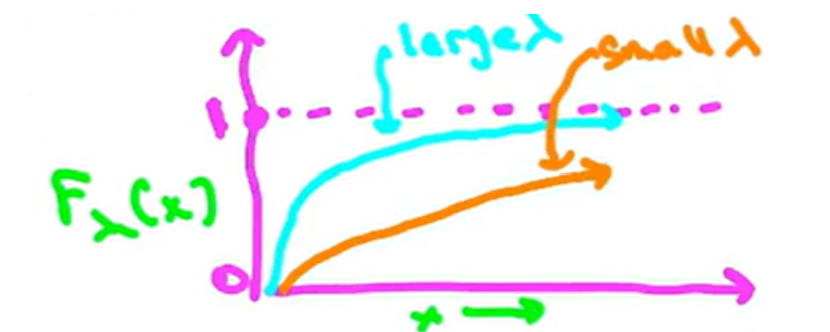
\includegraphics[scale = 0.5]{figures/f53.png}
    \caption{The graph of the CDF}
    \label{fig:mesh1}
\end{figure}\\

The above encapsulates the mechanism of biasing the credentials based on stake, resulting in adjusted credentials that follow a distribution conducive to fair leader selection. By incorporating this formula, the protocol achieves the objectives of both committee member selection and leader interpretation, ultimately leading to a balanced and robust PoS consensus mechanism. By using the exponential distribution transformation, the protocol achieves the goal of selecting leaders with a probability that is directly proportional to their stake. This ensures a fair and secure leader selection process, where participants are incentivized to stake more coins to increase their chances of being chosen as leaders.\\
The exponential distribution is intimately connected to the Poisson process. It represents the time between successive events in a Poisson process. In other words, if we consider the time between each email arrival in the inbox analogy, those time intervals could follow an exponential distribution.\\
Exponential distribution has a key property: if you have two independent exponential random variables with rates $\lambda_1$and $\lambda_2$ , the minimum of these two variables follows an exponential distribution with rate 
$\lambda_1 + \lambda_2$. This property is crucial for our understanding of adjusted credentials and leader selection.\\
Now, let's connect this to the concept of adjusted credentials. In the context of leader selection, adjusted credentials aim to ensure that the probability of being selected as a leader is proportional to a participant's stake. The choice of the exponential distribution in the formula for adjusted credentials is motivated by the property mentioned earlier.\\
When participants stake different amounts, their credentials need to be adjusted to achieve the desired proportional probability of selection. By using the exponential distribution transformation in the formula, we ensure that the adjusted credentials maintain the right distribution even when participants split their stake across multiple accounts.\\
This choice is elegant because it aligns with the Poisson process analogy. Just as the exponential distribution models time between events in a Poisson process, the adjusted credentials formula models the "time" it takes for a participant's stake to contribute to the minimum credential, reflecting the idea of leader selection over a distributed range of stakes.
\section{Proof-of-Stake Longest-Chain Protocols}
Here, we are going to get deeper into permissionless consensus, focusing on two prevalent approaches: Proof-of-Work and Proof-of-Stake. We will explore the concepts of longest chain protocols and BFT (Byzantine Fault Tolerance) protocols, discussing their integration with Sybil resistance. While Proof-of-Work was previously covered, we will now dive into Proof-of-Stake, its flexibility, and its relationship with longest chain consensus.\\
In chapter 9, we examined the Proof-of-Work approach, specifically longest chain consensus (Nakamoto consensus). We acknowledged the difficulties in coupling BFT protocols with Proof-of-Work, as it could lead to liveness issues due to hash rate fluctuations. However, Proof-of-Stake Sybil resistance can be combined with BFT consensus, making it a favorable migration path.

\subsection{Flexibility of Proof-of-Stake}
One of the notable advancements in the world of blockchain protocols is the advent of Proof-of-Stake (PoS) as an alternative to the traditional Proof-of-Work (PoW) consensus mechanism. PoS introduces a level of flexibility that can be effectively combined with various consensus protocols, making it a versatile choice for blockchain networks. In this section, we will delve deeper into the flexibility of PoS, how it can be integrated with different consensus approaches, and its impact on the evolution of blockchain protocols.

\subsubsection{PoS Coupled with BFT Protocols}
As we discussed earlier, PoS offers the unique advantage of being compatible with Byzantine Fault Tolerant (BFT) protocols. In contrast to PoW, which faces challenges when coupled with BFT techniques, PoS can seamlessly integrate with BFT consensus. This compatibility is rooted in the ability of PoS-based Sybil resistance to facilitate the fair selection of leaders, a crucial aspect of BFT protocols. This synergy has contributed to the migration from PoW to PoS in recent years, making PoS-based BFT protocols an increasingly preferred choice.

\subsubsection{PoS and Longest Chain Consensus}
What sets PoS apart is its adaptability not only to BFT protocols but also to the widely adopted Longest Chain Consensus approach. While PoW initially dominated this space, PoS has shown its ability to complement the Longest Chain Consensus paradigm. Early PoS blockchain protocols often utilized the longest chain approach, with Cardano being a prime example in 2023. This combination enabled the establishment of secure and robust networks while maintaining the principles of PoS-based Sybil resistance.

\subsubsection{Academic Landscape}
Interestingly, the academic exploration of PoS-based blockchain protocols has showcased a preference for longest chain protocols, as reflected in the research papers. This inclination could be attributed to various factors. First, the academic sphere may take time to catch up with practical implementations, leading to a bias toward earlier models. Second, BFT protocols might have been less explored and understood in the earlier stages of blockchain research. Nonetheless, the focus on longest chain protocols highlights their significance and potential for further innovation.

\subsubsection{Challenges and Research Opportunities}
Despite its inherent flexibility, PoS-based longest chain consensus presents its own set of challenges. Transitioning from PoW to PoS requires careful consideration, as the dynamics of leader selection, block proposals, and consensus verification differ substantially. The design of PoS-based longest chain protocols necessitates in-depth research and engineering efforts to ensure consistency, security, and liveness. As a result, the academic and research community is drawn to exploring the intricacies of PoS longest chain protocols, paving the way for valuable contributions to the blockchain ecosystem.
\subsection{Selection of Leaders}

In the context of implementing Proof-of-Stake longest chain consensus, the crucial aspect is the selection of leaders for each round. The leader selection process is designed to ensure that participants are chosen in a Sybil-resistant manner, allowing for a fair and secure proposal of blocks within the blockchain.\\
To achieve this, the protocol employs a mechanism based on verifiable random functions (VRFs) and associated credentials. Each participant in the network is tasked with computing their own credential using a VRF, a process that involves their private key. The output of this computation, referred to as the credential, serves as a key determinant in leader selection.\\
The VRF-based leader selection mechanism guarantees that participants cannot predict or manipulate the outcome of the selection process. This secrecy property is crucial for maintaining the security and integrity of the blockchain. Let's delve into the details of how this leader selection process unfolds:

\begin{enumerate}[label=\arabic*.]
    \item \textbf{VRF Evaluation:} In each time step of the protocol, every participant in the network evaluates a verifiable random function (VRF) using their respective private key. The input to this VRF is constructed by concatenating the current time step $t$ with a pseudorandom seed $r_{t}$ that corresponds to that time step. The VRF output, referred to as the credential, is unique to each participant due to the use of their private key.
    \item \textbf{Credential Interpretation:} The resulting credential for each participant is a numerical value that is specific to their private key, the current time step, and the associated pseudorandom seed. The next step is to determine the eligibility of participants for leadership roles based on their credentials. The protocol sets a threshold for credentials, below which a participant is considered eligible to be a leader for the current round.
    
    \item \textbf{Leader Eligibility:} The formula used to calculate the probability of leader eligibility is given by:
    
    $$1 - e^{-q_{i} \times \mu}$$
    
    where $Q_{i}$ represents the stake amount associated with participant $i$, and $\mu$ is the difficulty parameter. This formula ensures that participants with higher stake amounts have a greater likelihood of being selected as leaders. The rationale behind this design is to align leadership selection with participants' stake in the system, thereby incentivizing honest behavior.
    
    \item \textbf{Leader Selection:} Participants whose computed credentials fall below the threshold are considered eligible leaders for the current round. These selected leaders are granted the privilege to propose blocks for the blockchain in that particular time step. The threshold is set strategically to balance stake influence and ensure a controlled number of leaders per round.
    
    \item \textbf{Block Proposal Privilege:} Once selected as a leader, participants have the authority to propose blocks for the blockchain. Unlike Nakamoto consensus, where blocks come with predefined transactions and predecessor blocks, Proof-of-Stake longest chain consensus allows the proposing leader to freely choose transactions and even the preceding block they wish to extend.
\end{enumerate}
By using the verifiable random function approach, the protocol achieves Sybil resistance in leader selection. Participants' private keys and stake amounts contribute to the uniqueness and fairness of the selection process. The combination of VRF-based credentials and stake-dependent leader eligibility ensures that the system remains secure and resistant to manipulation.
\subsection{Finalizing Blocks}
In the Proof-of-Stake longest chain consensus framework, the process of finalizing blocks plays a crucial role in determining the state of the blockchain. Similar to other blockchain consensus protocols, such as Nakamoto consensus, the concept of finalization ensures the integrity and validity of transactions while allowing for the growth and extension of the blockchain.\\
In this context, finalizing blocks refers to the act of confirming the inclusion of a block in the blockchain with a high level of confidence. However, there are specific considerations and mechanisms that set Proof-of-Stake longest chain consensus apart from other protocols, and these are worth exploring.

\subsubsection{Block Proposal and Leader Selection}
Before diving into finalization, it's important to understand how block proposals are generated and how leaders are selected within the Proof-of-Stake longest chain consensus. Leaders, who are responsible for proposing blocks in each round, are chosen using a process that involves verifiable random functions (VRFs) and associated credentials.\\
Participants in the consensus protocol compute their credentials by evaluating VRFs using their private keys and a specific input derived from a pseudorandom seed. These credentials serve as "lottery tickets" that determine the probability of being selected as a leader for a given round. The probability of selection is influenced by both the participant's stake amount and a difficulty parameter (mu).

\subsubsection{Block Proposals and Flexibility}
Selected leaders have the privilege of proposing blocks in their respective rounds. Unlike some other consensus protocols, such as Nakamoto consensus, where each block proposal comes with fixed transactions and a predetermined predecessor block, Proof-of-Stake longest chain consensus offers a higher degree of flexibility.\\
In this protocol, leaders are not constrained to proposing a single block with fixed contents. Instead, they can propose multiple blocks, each extending different parts of the existing blockchain. This means that a leader can potentially propose a block that follows a different branch of the blockchain, creating a situation where competing blocks may emerge within the same round.

\subsubsection{Finalization and Block Depth}
Now, let's delve into the concept of finalizing blocks within the Proof-of-Stake longest chain consensus. Finalization is the process by which a block becomes considered as part of the confirmed and agreed-upon blockchain history. However, in this consensus protocol, the process of finalization comes with a unique twist.\\
Blocks are not immediately considered finalized as soon as they are proposed. Instead, the protocol introduces a parameter known as "$K$," which represents the number of blocks that need to follow a specific block in order for it to be considered finalized. In other words, a block is only truly confirmed and accepted by the network once it has a certain number of successor blocks.\\
This approach introduces a level of caution and security into the system. By requiring a block to have a certain depth of successors (at least $K$ blocks deep) on the longest chain, the protocol mitigates the risk of chain reorganization and fork-related issues. It ensures that transactions included in a block are unlikely to be reverted, providing users with a higher degree of confidence in the blockchain's history.
Here's an example for $K=2$:
\begin{figure}[h]
    \centering
    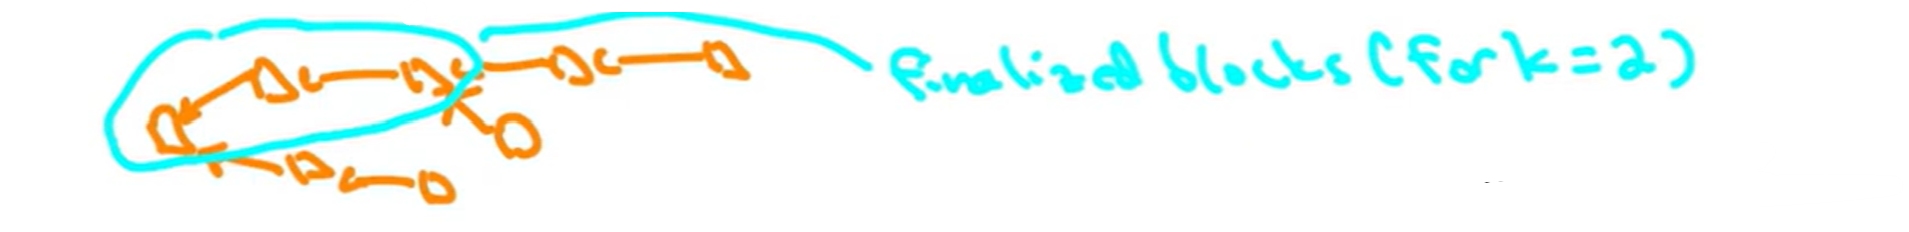
\includegraphics[scale = 0.5]{figures/f54.png}
    \caption{}
    \label{fig:mesh1}
\end{figure}\\

\subsubsection{Balancing Liveness and Consistency}
The parameter $K$ is a critical factor in striking a balance between liveness and consistency in the Proof-of-Stake longest chain consensus. A larger value of $K$ increases the level of finality and security, as it demands a more extended sequence of successors before considering a block as confirmed. However, a higher value of $K$ also introduces longer confirmation times for transactions.\\
Conversely, a smaller value of $K$ would lead to faster transaction confirmations but might also make the blockchain more susceptible to reorganizations. Determining the appropriate value of $K$ depends on various factors, such as the network's Byzantine fault tolerance, stake distribution, and desired trade-off between transaction speed and security.\\
Proof-of-Stake longest chain consensus combines verifiable random functions and longest chain protocols to achieve Sybil-resistant leader selection and block proposal. Challenges arise from the integration of these components, but the approach offers flexibility and security benefits.

\section{Issues with PoS Longest-Chain Protocols}
In the last section, we sketched what a proof-of-stake longest chain consensus protocol might look like. We aimed to reduce permissionless consensus to permissioned consensus, building upon our knowledge of permissioned longest chain consensus from chapter 8. Additionally, we explored techniques for Proof-of-Stake random sampling in Part 2 of this chapter. Here, we will combine these concepts to discuss a VRF-based approach to Proof-of-Stake random sampling.\\
However, it's important to note that in blockchain protocol design, things are rarely straightforward. Complications often arise, even when combining seemingly independent solutions. We observed this in the previous section as we discussed the protocol, revealing mismatches between the output of our VRF-based sampling and the expectations of permissioned longest chain consensus.\\
Let's delve into the issues that arise in this context.

\subsection{Variable Number of Winners in VRF-Based Sampling}
One significant challenge in VRF-based random sampling is dealing with the variable number of winners. While we can adjust a difficulty parameter to target a certain number of winners in a VRF sampling lottery, due to the randomness of the process, there will always be some variance in the actual number of winners. This variance can lead to cases where no winners are selected in a particular time step. The parameter $\mu$ which was previously introduced, is adjusted to target a certain number of winners in each sampling round. Ideally, each winner (or leader) would then be responsible for proposing a block during their designated time step.

\subsection{Issue 1: No Winners in a Time Step}
One of the challenges arising from VRF-based random sampling is the possibility of having no winners in a given time step. In some cases, no node's credential may be small enough to meet the threshold required for winning the VRF sampling lottery. As a result, there would be no designated leader for that particular time step. While this scenario may not be catastrophic, it does have implications for the protocol's performance.\\
For example, let's consider a situation where a time step passes without any leader being selected. Intuitively, this could be seen as a wasted opportunity. In contrast, having at least one leader in a time step allows for the advancement of the consensus protocol, as that leader can propose and confirm blocks. However, when there are no leaders, this progress is temporarily halted.\\
The absence of leaders in certain time steps has several repercussions. First, it impacts the latency of the protocol. Latency refers to the time it takes for transactions to be confirmed. If there are multiple time steps with no leaders, the overall confirmation time for transactions will increase. Transactions would need to wait for subsequent time steps with active leaders before they can be confirmed.\\
Secondly, this issue also affects the throughput of the protocol. Throughput refers to the rate at which transactions are processed and confirmed. When time steps pass without any leaders, the number of transactions being processed per second decreases. This reduction in throughput can lead to congestion and delays in transaction confirmation.\\
While these effects are undesirable, the good news is that the absence of leaders in certain time steps does not fundamentally compromise the basic guarantees of longest chain consensus. The protocol's consistency and liveness properties remain intact, ensuring that the blockchain continues to operate reliably and securely.\\
Despite the potential for some time steps to lack leaders, the overall functioning of the protocol remains robust and reliable, thanks to the mechanisms in place to handle other challenges.

\subsection{Issue 2: Byzantine Node Proposing Arbitrary Blocks with Arbitrary Predecessors}
In the context of proof-of-stake longest chain consensus, one notable issue arises from the potential behavior of Byzantine nodes. These malicious nodes possess the capability to propose multiple blocks in a single time step, and even more significantly, they can choose to extend the blockchain with these proposed blocks in a manner that does not adhere to the expected protocol rules. This behavior allows Byzantine nodes to create arbitrary branches in the blockchain, potentially leading to confusion and disruptions within the network.\\
For example if we currently have an
entry consisting of four blocks, nothing is stopping a Byzantine leader
from extending literally all four of these blocks with its own newly created four blocks(Figure 12.6).
\begin{figure}[h]
    \centering
    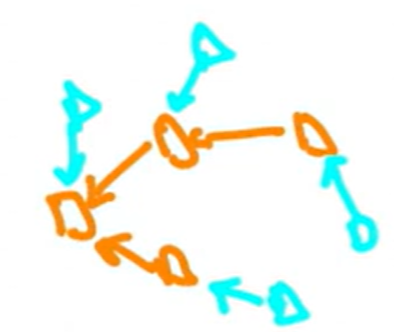
\includegraphics[scale = 0.5]{figures/f55.png}
    \caption{Example for issue 2}
    \label{fig:mesh1}
\end{figure}\\

\subsubsection{Byzantine Node's Influence on the Blockchain}
To illustrate this concept, consider the following scenario: The blockchain has already advanced to a certain point, characterized by a well-established longest chain. At a given time step, a Byzantine leader gains the opportunity to propose new blocks. However, instead of adhering to the protocol's rules, this Byzantine node can make arbitrary choices for the predecessors of its proposed blocks.\\
For instance, the Byzantine node could decide to extend multiple different parts of the existing blockchain simultaneously. It might propose blocks that extend some portions of the chain while ignoring others. The Byzantine node has the power to create multiple chains with arbitrary predecessors, effectively breaking the expected linear progression of the blockchain.\\


\subsubsection{Implications and Concerns}
This behavior raises concerns about the potential disruption and confusion it may introduce into the consensus process. Byzantine nodes, by proposing arbitrary blocks with arbitrary predecessors, can diverge from the normal operation of the protocol, leading to multiple competing versions of the blockchain. This situation could potentially lead to difficulties in determining the valid and authoritative version of the blockchain, thereby compromising the integrity and stability of the consensus mechanism.

\subsubsection{Drawing Parallels to Previous Discussions}
Interestingly, we can see similarities with discussions from earlier chapters, particularly chapter 8, which addressed similar challenges in the context of permissioned longest chain consensus. In that context, it was established that even under the influence of Byzantine nodes proposing multiple conflicting blocks, the fundamental properties of consistency and liveness could still be maintained under certain assumptions, such as the requirement for a significant percentage of honest participation and the adherence to a synchronous model.\\
Translating these insights to the proof-of-stake setting, similar principles hold true. Despite the potential for Byzantine nodes to propose arbitrary blocks with arbitrary predecessors, the underlying protocol design and the stipulated assumptions can ensure that the key properties of the longest chain consensus remain intact.

\subsection{Issue 3: Multiple Leaders in a Time Step}
In the context of the proof-of-stake longest chain consensus protocol, the occurrence of multiple leaders in a single time step presents a significant challenge. This situation arises when more than one node is granted the authority to propose blocks at the same point in time. While this phenomenon is not inherently problematic, it introduces certain complexities and considerations that need to be addressed within the protocol's design.

\subsubsection{Addressing Multiple Honest Leaders}
The presence of multiple leaders in a time step can lead to situations where honest nodes propose blocks that extend different parts of the blockchain. This introduces the potential for conflicting block proposals, as different honest nodes may independently extend different branches of the blockchain. This scenario can appear worrisome, as the contributions of honest nodes might cancel each other out or lead to potential forks in the blockchain. However, by carefully selecting the protocol's parameters, this issue can be managed effectively.

\subsubsection{The Role of the Difficulty Parameter $\mu$}
To mitigate the impact of multiple leaders proposing conflicting blocks, we can try adjusting a parameter known as $\mu$. This parameter is a key element in the protocol, influencing the behavior of the blockchain's consensus mechanism.\\
By setting $\mu$ to a sufficiently small value, the protocol aims to reduce the likelihood of having multiple leaders active in the same time step. In other words, a smaller $\mu$ reduces the probability of encountering situations where more than one honest node proposes blocks simultaneously.

\subsubsection{Ensuring Consistency and Liveness}
With an appropriately chosen value of $\mu$, the impact of multiple honest leaders proposing conflicting blocks can be minimized. While some contributions might still be wasted due to the presence of competing block proposals, the overall consistency and liveness guarantees of the longest chain consensus protocol are not compromised.\\
The rationale behind this conclusion lies in the fact that by keeping $\mu$ small, the protocol aims to ensure that the occurrence of multiple honest leaders in the same time step remains infrequent. Consequently, any disruptions caused by this scenario are limited in scope and do not undermine the core guarantees provided by the protocol.

\subsection{Comments on Proof-of-Stake Longest Chain Protocols}
Now, we will provide some comments on the proposed Proof-of-Stake longest chain protocol, highlighting interesting connections and nuances. These comments are optional and are meant to provide additional insights into the design and implications of the protocol.
\subsubsection{\#1: PSL FLM Impossibility Theorem}
The PSL FLM (Public Key Infrastructure, Longest Chain, FLM) Impossibility Theorem is a significant result, which explores the impact of the Public Key Infrastructure (PKI) assumption on achieving consensus within a blockchain protocol. This theorem was the subject of chapter 3 and builds upon concepts introduced in previous chapters.\\
To comprehend the implications of the PSL FLM Impossibility Theorem, it's essential to recall the context established in chapter 2. In that chapter, the Dollar Strong Protocol was presented, demonstrating the achievement of consensus even in the presence of 99 Byzantine nodes under the synchronous model. This remarkable feat was accomplished by relying on the PKI assumption, which implies that the protocol has prior knowledge of the public keys of all participating nodes.\\
The PSL FLM Impossibility Theorem shifts the focus to a scenario where the synchronous model is maintained, but the protocol lacks a priori knowledge of the public keys of the nodes involved. This absence of PKI introduces a challenge to achieving consensus effectively. The theorem highlights that without the PKI assumption, it becomes impossible to ensure consensus if a third or more of the nodes in the network are Byzantine, meaning they can act maliciously.\\
The core of the impossibility proof revolves around a concept known as the "hexagon argument". This argument asserts that in the absence of PKI, Byzantine nodes could exploit the lack of predetermined knowledge about public keys to subvert the consensus process. The hexagon argument illustrates that Byzantine nodes could propose conflicting blocks using different public keys, leading to a breakdown in the coherence of the blockchain's state.\\
However, there exists a silver lining in the form of a positive result: if the proportion of honest nodes exceeds two-thirds, consensus can still be achieved even without the PKI assumption. This outcome provides a ray of hope in a scenario where a substantial majority of nodes operate honestly. Nevertheless, it's essential to note that the specific details of this positive result are of less immediate importance for the discussion at hand.\\
An intriguing observation arises when comparing the PSL FLM Impossibility Theorem with the context of longest chain protocols. Throughout this chapter, we have emphasized the significance of the 50\% threshold for honest participation in longest chain protocols. This threshold denotes the proportion of honest nodes required to ensure consistent and live blockchain behavior in the synchronous model.\\
A noteworthy point of confusion emerges when trying to reconcile the positive result of achieving consensus without PKI for more than two-thirds honest nodes with the negative result of the PSL FLM Impossibility Theorem. This confusion is especially pronounced in the context of Nakamoto consensus, which operates without a PKI assumption and yet achieves guaranteed consistency and liveness with 51\% honest hash rate.\\
The resolution of this apparent contradiction lies in the unique characteristics of Nakamoto consensus, particularly the nature of proof-of-work (PoW) mechanisms. PoW restricts Byzantine nodes' ability to propose multiple blocks in a single round by tying block proposals to the solution of cryptographic puzzles. This restriction diminishes the power of Byzantine nodes and contributes to Nakamoto consensus's ability to tolerate a higher proportion of Byzantine nodes than implied by the PSL FLM Impossibility Theorem.


\subsubsection{\#2: No Difficulty Adjustment Necessary in Proof-of-Stake}
Another interesting aspect to consider is the absence of a difficulty adjustment mechanism in Proof-of-Stake (PoS) protocols, which sets PoS apart from Proof-of-Work (PoW) systems. In PoW, a key feature is the dynamic adjustment of difficulty levels to ensure a consistent block generation rate, typically around once every 10 minutes. This adjustment accounts for changes in hash rate and maintains the protocol's stability.\\
However, in PoS, the situation is different. While the total amount of stake in the staking contract is still a critical factor, PoS protocols do not require the complex difficulty adjustment seen in PoW. Instead, PoS protocols focus on the observable total stake, represented as the sum of stake amounts from validators. Notably, this total stake amount can change over time, but the protocol is always aware of these changes as they occur.\\
This simplification leads to a key consequence in PoS longest chain protocols. In PoW, the concept of the "longest chain" is intricately linked to the cumulative amount of work done, measured by the difficulty-adjusted block count. However, in PoS, the definition of the "longest chain" becomes much more straightforward: it is the chain with the largest number of blocks. This is because the protocol's internal adjustments, which account for changes in total stake, inherently regulate block generation without requiring a separate difficulty adjustment mechanism.\\
It's worth noting that this simplification applies not only to the proposed PoS longest chain protocol but also extends to other PoS blockchain designs. This distinction highlights the inherent differences between PoW and PoS consensus mechanisms and showcases how PoS avoids the complexity of dynamic difficulty adjustment.

\subsubsection{\#3: Leader Selection}
An insightful comparison can be drawn between Proof-of-Work (PoW) and Proof-of-Stake (PoS) mechanisms, particularly in their approaches to leader selection. While both PoW and PoS serve as consensus mechanisms within blockchain protocols, they diverge in how they identify individuals authorized to propose new blocks and validate transactions.\\
In the PoW context, leader selection hinges on participants engaging in a competitive process to solve a computational puzzle. This intricate puzzle is intentionally designed to demand significant computational resources for its solution. The participant who successfully cracks the puzzle first is granted the privilege of proposing the next block, alongside a reward of newly minted cryptocurrency and transaction fees.\\
The PoW puzzle serves a dual purpose: it thwarts potential Sybil attacks by necessitating substantial computational power, and it introduces scarcity by mandating extensive computational effort. The computational exertion required to solve this puzzle is referred to as "mining", and it functions as proof that the participant has invested genuine computational resources.\\
Contrastingly, PoS adopts an alternative approach to leader selection. Rather than engaging participants in computational races, PoS designates the task of block proposal to validators based on their "stake" within the network. Stake denotes the amount of cryptocurrency held by a participant, which is then locked up as collateral within the system. Validators are determined either deterministically or pseudorandomly, often taking into account their stake and additional factors.\\
PoS introduces a novel concept termed the "credential". This credential is established using a verifiable random function (VRF), which generates a unique identifier for a validator at a specific time step. Unlike the PoW approach where participants grind through various inputs to discover a winning hash, PoS strives to minimize grinding efforts, thereby reducing computational demands.\\
A key distinction between PoW and PoS lies in the inputs to the leader selection process. In PoW, a lottery ticket incorporates multiple fields, such as the proposed block, a pointer to the preceding block, the proposer's public key, and a nonce. Collectively, these fields dictate whether a participant secures the right to propose a block. The nonce enables participants to engage in grinding, iterating through different possibilities to identify a winning combination.\\
In PoS, the inputs to the leader selection process are streamlined. Validators generate a credential using their private key ($sk_i$), the current time step, and a pseudorandom seed. This credential serves as evidence of their eligibility to propose a block. Crucially, the proposed block and its predecessor are excluded from the input at this stage.\\
This division between block proposal and credential presentation in PoS bears significant implications. In PoW, once a participant's lottery ticket secures a win, the block they propose is predetermined by the winning hash. Conversely, in PoS, a validator who attains a winning lottery ticket subsequently possesses the liberty to freely designate both the proposed block and its predecessor. This autonomy allows for heightened flexibility in proposing blocks but also introduces challenges, including the potential for multiple conflicting proposals based on the same triumphant credential.

% \nt{\noindent
% \textbf{PoW:} leader \iff $\text {h}(B || pred ||pk_i|| nonce)$ is sufficiently small\\
% \noindent
% \textbf{PoS:} leader \iff $\text{VRF}_{sk_i}(t || r_t)$}

\subsection{Ensuring Valid Proposals in PoS}
In the Proof-of-Stake (PoS) protocol, validators play a crucial role in ensuring the validity of proposed blocks. This involves a series of checks and verifications to maintain the integrity of the consensus process. Let's delve into the steps validators take to validate proposed blocks and prevent malicious behavior.\\
First and foremost, validators need to verify the legitimacy of the credentials presented by the proposer. The credential is computed using a verifiable random function (VRF) and is a critical component in determining whether a validator is eligible to propose a block. Validators ensure that the credential's computed value matches the public key of the proposer and the output of the VRF. This step is essential to prevent forged credentials and unauthorized block proposals.\\
To determine the legitimacy of the proposed block, validators also compare the proposer's credential against a predefined threshold. This threshold is a function of the protocol's difficulty parameter $\mu$ and the validator's stake amount. If the computed credential is below this threshold, it indicates that the proposer is indeed eligible to propose a block for the given time step. This comparison helps ensure that only validators with sufficient stake and the necessary cryptographic proof can participate in the block proposal process.\\
Furthermore, validators must verify the proposed block and its predecessor using cryptographic signatures. When a validator wins the lottery and intends to propose a block, they sign both the proposed block and its predecessor with their private key. Other validators receiving the proposal can then verify these signatures using the corresponding public key. This step prevents malicious actors from hijacking legitimate credentials and proposing unauthorized blocks or predecessors.\\
Consider a scenario where a validator, Alice, wins the lottery and proposes a new block for the current time step. She generates her credential using the VRF with her private key, public key, and input data. After confirming the legitimacy of her credential, other validators assess whether the credential value is below the threshold determined by $\mu$ and Alice's stake amount.\\
Assuming the credential passes this threshold test, validators proceed to verify the proposed block and predecessor. Alice signs both the proposed block and its predecessor using her private key, ensuring the authenticity of her proposal. Validators receiving Alice's proposal can then verify these signatures against her public key. This multi-step verification process guarantees that the proposed block is legitimate and adheres to the protocol's rules.

\section{Further Discussion of PoS LC Protocols}
\subsection{Review}
In this section, we delve into the intricate realm of Proof-of-Stake longest chain protocols, marking the culmination of our exploration in part three of chapter 12. This section serves as the final installment dedicated to the profound concept of Proof-of-Stake longest chain protocols, following our previous engagements with the challenges posed by Proof-of-Stake random sampling and permissioned consensus.\\
As we reflect on the journey so far, we're reminded that the road to consensus is not as straightforward as it may initially seem. Part two of our discourse illuminated the complexity underlying Proof-of-Stake random sampling, highlighting that achieving consensus in such settings is far from a trivial task. Moreover, the earlier sections underscored that even permissioned consensus, though seemingly more structured, is not immune to its own set of challenges.\\
Venturing into part three, we encountered the ambitious aspiration of amalgamating different techniques into T-type protocols. However, the union of these approaches is not a seamless endeavor. Each layer of complexity compounds the overall intricacy of the protocol, ultimately giving rise to a host of additional challenges.\\
Now, we stand at the precipice of comprehending Proof-of-Stake longest chain protocols. As we delve deeper, we find ourselves entangled in a web of complexities that surpass the boundaries of their predecessors. While we previously dissected several issues in the last section, it's crucial to recognize that these issues were examined under a strong assumption – the existence of an ideal Randomness Beacon. However, it is essential to acknowledge that this assumption is far from realistic in practical deployments. In the real world, the notion of an ideal Randomness Beacon remains elusive, challenging the feasibility of such an assumption. Consequently, any concrete implementation of the protocol must grapple with approximations and real-world constraints.\\
One potential avenue, harkening back to our exploration in part two, involves the deployment of advanced techniques, such as two-phase protocols intertwined with verifiable delay functions. While this may hold promise for the future, it's worth noting that as of early 2023, these approaches remain experimental, lacking the extensive battle-testing that is often indicative of mature technologies.
Given this context, the focus of this section shifts to a pragmatic examination of the prevailing best practices that have emerged in the realm of serious Proof-of-Stake longest chain protocols. These practices pivot around the utilization of a pseudorandom seed, intricately derived from the current state of the blockchain. Throughout our discussions, we've encountered diverse methods for generating a pseudorandom seed from the blockchain state. It's worth emphasizing that the chosen methodology for this derivation holds significance, as certain approaches offer superior outcomes compared to others. To ensure continuity with our preceding discourse, let's consider a scenario where we adopt the same methodology employed in the credential of the most recent block proposer.\\
The term "credential" refers to a private computation executed by each owner of a public key to determine their eligibility as a round leader. This computation involves the evaluation of a verifiable random function (VRF), utilizing the appropriate private key. This private key is combined with a concatenated input consisting of the time step and the pseudorandom seed specific to that time step. In the context of referencing the credential of a previous block, we envision an output from the VRF executed with a specific private key and time step, accompanied by the corresponding pseudorandom seed. While an optional step involves subjecting this credential to a cryptographic hash function, yielding an outcome that effectively behaves as a random number within the range of zero to one, for the sake of clarity, we shall temporarily set this aspect aside.\\
Our exploration of this pseudorandom seed does not occur in isolation. Rather, it has been a recurring motif throughout our journey. The concept was first introduced in part two, where we laid the groundwork for its utilization. Subsequently, in the initial stages of part three, we harnessed this idea in conjunction with Byzantine fault-tolerant (BFT) type protocols.\\
However, a drawback emerges as we traverse this path: the susceptibility of this type of pseudorandom seed to manipulation. This vulnerability stems from the ability of nodes participating in the protocol to influence and manipulate the pseudorandom seed. An illustrative attack involves the division of stake among multiple sybils, each endowed with its own public key-private key pair. With this setup, each sybil receives a distinct credential during each time step.\\

\subsection{Pseudorandom Seed Manipulation}
Pseudorandom seeds are derived from the blockchain state and play a crucial role in determining the randomness used in the protocol. However, malicious actors can attempt to exploit the process of seed derivation for their advantage.\\
Consider the scenario where an attacker possesses a significant amount of stake and wishes to manipulate the protocol. To achieve this, the attacker may distribute their stake across multiple identities, or "sybils", each associated with its own public-private key pair. At each time step, these sybils generate their own credentials using the verifiable random function (VRF), with the intention of producing low credentials for some of them.\\
The attacker's goal is to have multiple sybils with sufficiently low credentials to qualify as block proposers. This situation occurs periodically, and during such time steps, the attacker faces a crucial decision. They must select which sybil's credentials to use for proposing a block, aiming to maximize their influence on the protocol.

For instance, imagine that two of the attacker's sybils have exceptionally low credentials at a particular time step. This presents the attacker with an opportunity to choose between these two sybils for block proposal. The selected credential then becomes part of the pseudorandom seed used for subsequent time steps.

\subsubsection{Consequences of Credential Selection}
By strategically choosing between the available credentials, the attacker not only influences the current block proposal but also impacts the pseudorandom seed that guides future protocol behavior. This manipulation introduces an inherent bias into the protocol's operation, potentially allowing the attacker to steer the system towards their desired outcomes.\\
This phenomenon raises concerns about the integrity and fairness of the protocol. The manipulation of pseudorandom seeds has the potential to compromise the underlying principles of Proof-of-Stake protocols, where security and consensus are expected to be achieved through decentralized and unbiased mechanisms.

\subsubsection{Mitigation Strategies}
To address the challenge of pseudorandom seed manipulation, there are potential mitigation strategies. One approach is to derive the pseudorandom seed not solely from a single block's credential but from a collection of recently proposed blocks' credentials. This method aims to dilute the influence of individual sybils by considering a broader range of contributors to the seed derivation process.\\
By concatenating the credentials of a significant number of recently finalized block proposers and processing them through a cryptographic hash function, a more balanced and less manipulable pseudorandom seed may be generated. This approach reduces the impact of low-credential sybils on the protocol's operation.

\subsection{Previous Block Credentials}
In the context of Proof-of-Stake longest chain protocols, a critical consideration arises regarding the selection of the pseudorandom seed for each new block proposal. While the idea of using pseudorandom seeds derived from the blockchain state seems promising, there is a notable complication introduced by the choice of the previous block's credentials.

\subsubsection{Pseudorandom Seed and Predecessor Block}
The pseudorandom seed plays a crucial role in determining the block proposer and subsequent actions in the protocol. It is derived from the blockchain state and is influenced by the credentials of the previous block's proposer. This introduces a dependency on the choice of the predecessor block, impacting the entire protocol's behavior.\\
This dependence is not immediately evident in the process. The pseudorandom seed is not explicitly fed into the verifiable random function (VRF) with the previous block's credentials. Instead, the VRF input is determined by the concatenation of the time step and the pseudorandom seed for that time step. However, the choice of the predecessor block implicitly determines the pseudorandom seed, thus leading to an indirect connection.\\
This means that at each time step, the protocol participants effectively receive a collection of independent lottery tickets, one for each potential choice of the predecessor block. The winner of the lottery gains the right to propose the next block and, in turn, influences the pseudorandom seed for subsequent time steps. Consequently, there is an incentive for participants to carefully consider and potentially manipulate their choice of predecessor block to maximize their chances of winning the lottery and extending their influence.\\
To grasp the implications of this dependency, consider the scenario of an attacker attempting to manipulate the protocol to their advantage. The attacker is trying to orphan a target block within the blockchain. Initially, the attacker has an interest in two distinct lottery tickets, each associated with a different block preceding the target. These lottery tickets allow the attacker to potentially extend alternative chains that could lead to orphaning the target block. However, with the introduction of the pseudorandom seed's dependency on the choice of predecessor, the attacker's strategy becomes more intricate.\\
The attacker's progress is twofold: Firstly, by extending an alternative chain, the attacker gets one step closer to potentially overtaking the honest chain. Secondly, and more subtly, the attacker gains an increased number of independent lottery tickets for future time steps.\\
In the example, the attacker starts by extending blocks that precede the target, creating an alternative chain. At each time step, the attacker has multiple lottery tickets corresponding to different blocks. As time progresses, the attacker's set of lottery tickets increases, encompassing both previously targeted blocks and any new ones.

\subsubsection{Implications for Protocol Guarantees}
The expansion of the attacker's lottery tickets has significant implications for the guarantees provided by the protocol. While in the case of an ideal Randomness Beacon, the protocol's security threshold remains at 50\%, the situation changes with pseudorandom seeds.\\
Remarkably, a paper titled "Nakamoto Always Wins" introduces a non-trivial probabilistic analysis, revealing that the threshold for maintaining consensus under pseudorandom seeds is approximately 73\%. This means that an attacker with control over at least 27\% of the stake could potentially disrupt the protocol's guarantees of consistency and liveness.
\subsection{Order of Operations}
When $r_t$ represents genuinely random bits that are entirely independent of any manipulation, an owner of a public key obtains a unique credential at each time step. This uniqueness arises because the private key, time step, and random seed are predetermined and unalterable. Consequently, the owner cannot manipulate their private key, time, or the random seed. This results in a single lottery ticket per time step, with no influence over block proposals. Under this ideal scenario, the lottery winner can propose blocks extending any part of the blockchain, leading to simultaneous extensions.\\
However, when $r_t$ is derived pseudorandomly from the preceding blockchain blocks, a new dynamic emerges. Although the predecessor block is not directly used as input in the verifiable random function (VRF) for generating credentials, the choice of predecessor block indirectly determines the pseudorandom seed fed into the VRF. This introduces a subtle yet significant change: the attacker now gains the ability to create multiple independent lottery tickets, each corresponding to a potential predecessor choice.\\
To illustrate this concept, let's consider a simplified scenario. Imagine a blockchain with a single chain, and the attacker aims to orphan a target block to execute a double spend. Honest nodes extend the magenta chain, while the attacker seeks to extend both the magenta and an alternative orange chain leading up to the target block.\\
Initially, the attacker's goal is to extend the magenta blocks just preceding the target. At each time step, the attacker possesses two distinct lottery tickets, each associated with a magenta block. Progress may be slow as the attacker competes against the honest nodes extending the magenta chain.\\
However, the introduction of an orange block changes the dynamics. With the orange block at the same height as the magenta blocks, the attacker gains an additional lottery ticket for each time step. This leads to increased chances of obtaining winning lottery tickets in subsequent time steps, as the attacker's potential block extensions grow.\\
In the next time step, the attacker now possesses three distinct lottery tickets: two for the magenta blocks and one for the orange block. Although extending the same magenta block as before may seem redundant, it serves to further amplify the attacker's lottery ticket count. Consequently, the attacker gains a higher probability of generating additional blocks in the future.\\
This distinction between ideal Randomness Beacon and pseudorandom seed scenarios leads to a critical observation. While the former scenario maintains consistent guarantees and liveness with an honest majority of over 50\%, the latter case significantly alters the security threshold. A non-trivial probabilistic analysis, as demonstrated in the paper "Nakamoto always wins", reveals that the necessary honest majority for consensus in pseudorandom seed protocols is approximately 73\%, a significant departure from the traditional 50\% threshold.
\subsection{Unruly Random Process}
The concept of the unruly random process might initially seem complex to grasp. It revolves around the attacker's continuous acquisition of lottery tickets, and the subsequent extension of chains wherever possible. This dynamic growth may appear chaotic, but despite its seemingly disorganized nature, it can be succinctly explained.\\
From the attacker's perspective, the advantage lies in its capacity to expand independent parallel chains. If any of these parallel chains surpasses the length of the honest chain, the attacker achieves victory. Interestingly, this scenario can be distilled down to a simpler representation. The attacker gains the equivalent benefit of possessing a single chain with a stake multiplied by a factor of \(e\), where \(e\) represents the base of the natural logarithm, approximately equal to 2.718.\\
The emergence of the factor \(e\) can be attributed to the compounding effects that transpire over time as the attacker cultivates multiple independent branches. While the precise origin of this factor may seem intricate, its significance becomes clearer in its implications. If we accept this factor as part of the analysis, we can discern the reasoning behind the 73 percent threshold.\\
To delve into this further, let's introduce a variable, denoted as \(\alpha\), representing the fraction of stake controlled by Byzantine nodes. This context reveals that Byzantine nodes effectively possess a stake of \(e \times \alpha\), while honest nodes hold the remaining portion of the stake, which can be calculated as \(1 - \alpha\). The pivotal condition for the attacker's success is when its sped-up stake (\(e \times \alpha\)) overtakes the stake held by honest nodes (\(1 - \alpha\)). This can be expressed as an inequality:

$$
e \times \alpha > 1 - \alpha
$$

Rearranging this inequality unveils the pivotal criterion for a successful attack: \(\alpha > \frac{1}{e + 1}\), which approximates 27 percent.\\
A fascinating observation arises here: even if Byzantine nodes control around 27 or 28 percent of the total stake, the probability of a single chain proposed by the attacker overtaking the honest chain remains extremely low. However, an intriguing phenomenon occurs when the attacker gains the ability to generate an exponentially large number of competing chains. In such a scenario, the likelihood of one of these chains achieving a "Super Lucky" status and surpassing the honest chain becomes notably higher. This underscores the significance of the 27 percent threshold – a seemingly arbitrary number rooted in intricate mathematical underpinnings. Notably, this vulnerability exposes the potential for an attacker with 28 percent of the overall stake to execute double-spending attacks, highlighting a critical limitation of this specific proof-of-stake longest chain design.\\
In essence, the discussion underscores the vulnerability of the proof-of-stake longest chain design when a significant fraction of the stake falls under Byzantine control. Although the threshold of 27 percent may appear arbitrary, it has practical implications and highlights the need for more robust protocols to mitigate the risks associated with Byzantine control.

\subsectionExtreme Random Process{}
The concept of the "Extreme Random Process" may sound unconventional and even counterintuitive at first. This approach involves a unique scenario where all the pseudorandom seeds ($r_t$) are made exactly the same, akin to a constant value. This might seem strange or even radical, but upon closer examination, there are interesting aspects to consider.\\
Even in this extreme case, each participant in the protocol still receives a non-trivial set of credentials at every time step. Recall that the credential is generated by evaluating the VRF (Verifiable Random Function) using the corresponding private key and the concatenation of the time step and the pseudorandom seed. In this case, the pseudorandom seed is essentially eliminated, reducing the process to the VRF evaluated at the time step itself. This may appear to negate the randomness, but it's important to remember that every participant evaluates the VRF with their unique private key, resulting in different credentials for each.\\
This feature of receiving different credentials per participant highlights a sense of non-craziness in the extreme scenario. Additionally, it offers an intriguing advantage: the elimination of manipulability. Since the pseudorandom seeds effectively don't exist, no participant has the opportunity to manipulate them. This aspect contributes to a certain level of security against manipulation attempts.\\
However, there is a significant drawback to this extreme approach, similar to a concern discussed earlier in Part Two of this chapter. It relates to the predictability of future credentials. Without the influence of ideal pseudorandom seeds or their dependence on blockchain state, the future credentials become predictable to a certain extent. This issue is reminiscent of a proposal from earlier in this chapter, where credentials could be predicted due to a lack of dependence on randomness.\\
The predictability issue has implications, especially when it comes to security concerns. For instance, an attacker could engage in what's known as "grinding" on public-private key pairs. This involves generating new key pairs until one is found that yields favorable VRF outputs during specific time periods. This approach could be used for malicious purposes, such as orchestrating double spend attacks during windows of time when credentials are advantageous for an attack.\\
A potential solution to this predictability problem could involve forcing participants to commit to their public-private key pairs before learning about the pseudorandom seed $r_t$. However, in this extreme scenario, all $r_t$ values are known when the protocol is deployed, making any attempt at a warm-up period ineffective in preventing predictability-based attacks.\\
Additionally, coupling this approach with Byzantine Fault Tolerant (BFT) consensus protocols could introduce what is termed as "riskless forking attacks". These attacks involve creating alternative chains that roll back previously finalized blocks, which could lead to double spend scenarios or other disruptions in the network.\\
Furthermore, the extreme approach poses challenges when integrated into a longest chain consensus protocol. The risk of riskless forking attacks remains a concern, and the high predictability of future credentials can facilitate certain types of attacks that compromise the integrity of the blockchain.\\
To mitigate these challenges and strike a balance between predictability and security, a hybrid solution is proposed, as discussed in the subsequent sections. This hybrid approach aims to address the limitations of both extreme cases while maintaining essential aspects of the protocol's security and functionality.

\subsection{Preductability}
The predictability of pseudorandom seeds can lead to undesirable consequences, such as enabling malicious actors to anticipate their future credentials, potentially allowing them to manipulate the protocol.\\
In the initial exploration of pseudorandom seeds, an extreme case was discussed where all pseudorandom seeds ($r_t$) are set to a constant value, independent of the blockchain state. While this may seem counterintuitive, it has some intriguing aspects. For instance, if $r_t$ is fixed for all blocks, the predictability of future credentials becomes straightforward. The owner of a particular public key can accurately foresee their credentials at any future time step, as they are evaluating the VRF (Verifiable Random Function) with a consistent input.\\
This predictability, however, has significant downsides. It opens the door to manipulation and strategic behavior. A malicious actor could repeatedly generate public-private key pairs until finding a pair that yields favorable future VRF outputs. This manipulation undermines the integrity of the system and jeopardizes security.\\
Moreover, when predictability is widespread, it introduces an even more concerning problem. Malicious actors can anticipate future time steps where they are likely to be leaders and can propose blocks. This insight allows them to orchestrate double spending attacks or other malicious activities during these advantageous periods, causing serious disruptions.\\
To counter these predictability-related issues, the protocol designers propose a compromise in the form of a "hybrid solution". This approach aims to strike a balance between complete predictability and independent randomness, ensuring the security of the Proof-of-Stake longest chain protocol.\\

\subsection{Hybrid Solution}
In order to address the challenges posed by the extremes of having constant pseudorandom seeds for all blocks or fully independent seeds, a hybrid solution is proposed. This approach aims to strike a balance between the two, introducing a parameter denoted as L, which signifies a reset interval. The central idea here is to periodically reset the pseudorandom seeds to ensure that predictability is bounded within certain limits. Let's delve into the details of this innovative approach.

\subsubsection{The Concept of Reset Interval (L)}
The concept of the reset interval revolves around the idea of periodically refreshing the pseudorandom seeds used in the protocol. This is achieved by defining the pseudorandom seed $r_t$ based on the credential of the proposer of the most recent block at a height that is a multiple of L. To illustrate this concept, consider an example with concrete values:\\

Suppose we choose L to be 1000. This means that the pseudorandom seed $r_t$ will be determined by the credential of the proposer of the block at height 9000, assuming we're currently proposing a block at height 9723. This ensures that the pseudorandom seed is refreshed every L blocks, creating distinct intervals of predictability.

\subsubsection{Correlated and Independent Lottery Tickets}
The hybrid solution combines two different modes of generating lottery tickets: correlated and independent. Within a group of blocks defined by the reset interval L, the pseudorandom seed remains constant, leading to correlated lottery tickets. This means that all blocks within the same interval have identical pseudorandom seeds, influencing their credentials. Let's visualize this:\\

Imagine a scenario where we have the Genesis block on the far left. At block height 9000, there are three blocks created. These blocks naturally fall into three distinct groups, each associated with one of the blocks at height 9000. Blocks proposed at heights greater than 9000, but within the same group, share the same pseudorandom seed $r_t$.\\
On the other hand, across different groups, the pseudorandom seeds are different. This is because the blocks at height 9000, which serve as the basis for determining $r_t$, have distinct credentials for each group. The following diagram illustrates this idea:
\begin{figure}[h]
    \centering
    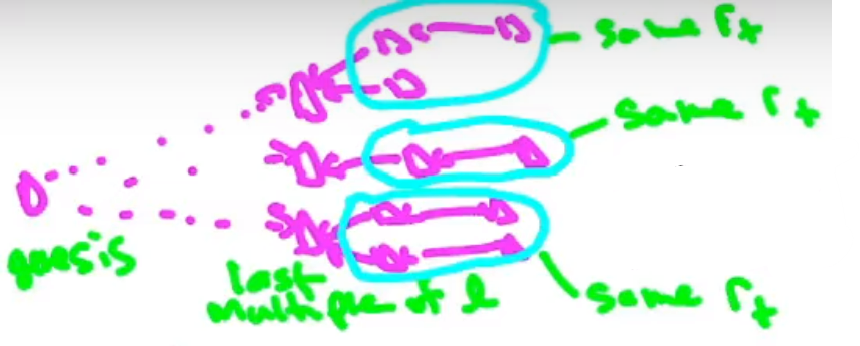
\includegraphics[scale = 0.5]{figures/f56.png}
    \caption{Diagram: Genesis block $\rightarrow$ Block Height 9000 (Group 1) $\rightarrow$ Block Height 10000 (Group 1) $\rightarrow$ Block Height 11000 (Group 1) ...}
    \label{fig:mesh1}
\end{figure}\\
This hybrid mechanism ensures that, within a group, blocks share correlated lottery tickets due to their common pseudorandom seed. However, the pseudorandom seeds vary between different groups, leading to independent lottery tickets.

\subsubsection{Balancing Predictability and Security}
The hybrid solution achieves a delicate balance between predictability and security. Predictability is limited to a bounded duration determined by the reset interval L. During this time, participants can anticipate their future credentials and likelihood of being a leader. For instance, if L is set to 1000 and a warm-up period is implemented, participants can predict their credentials for the next 1000 blocks.\\
While the hybrid approach does not eliminate all challenges of predictability, it provides a controlled and manageable form of predictability. The predictability window is well-defined and limited, preventing long-term exploitation of predictable patterns.

\subsubsection{Slowing Down Attacker's Growth of Independent Chains}
An essential benefit of the hybrid solution is its ability to significantly slow down an attacker's growth of independent chains. In the case of fully independent seeds, the attacker's chains could grow exponentially, posing a security risk. However, with the hybrid approach, the attacker's capacity to create multiple independent chains is restrained by the reset interval L.\\
Within a group, where blocks share correlated lottery tickets, the attacker's opportunities for exponential growth are limited. The correlation among blocks in the same group mitigates the attacker's ability to create a multitude of independent chains. This feature is crucial for maintaining the integrity of the protocol and safeguarding against attacks.

\subsubsection{Convergence to Traditional Behavior}
Interestingly, the hybrid solution provides a pathway to recover the familiar behavior of Proof-of-Stake protocols with a 51 percent threshold. As the reset interval L becomes larger, the protocol's behavior converges toward the scenario where 51 percent of honest stake suffices to ensure provable consistency and liveness. In other words, by adjusting L, the protocol's security and guarantees can be tuned to meet specific requirements.

\subsection{Independent Lottery Tickets}
The idea of "Independent Lottery Tickets" is crucial in understanding the dynamics of the proposed hybrid solution for Proof-of-Stake longest chain protocols. This concept revolves around the generation of lottery tickets that determine the ability of nodes to extend chains and propose blocks. The hybrid solution seeks to strike a balance between two extremes: constant pseudorandom seeds and fully independent seeds.\\
When we talk about "lottery tickets", we're referring to the credentials that nodes possess to participate in the block proposal process. These credentials are based on pseudorandom seeds that are used to determine the order in which nodes propose blocks and extend chains.\\
In the extreme scenario of constant pseudorandom seeds, all nodes would use the same seed for generating their credentials. This means that every node's ability to propose a block or extend a chain would be entirely predictable. Since everyone has the same credentials, there's no randomness involved, and this predictability undermines the security and fairness of the system. If an attacker knows the credentials of all nodes, they can strategize to manipulate the block proposal process.\\
On the other hand, the concept of "Independent Lottery Tickets" aims to inject randomness into the process. This randomness is crucial to prevent predictability and manipulation by attackers. In the context of the hybrid solution, independent lottery tickets ensure that an attacker's ability to grow competing chains is restricted and controlled.\\
To illustrate this concept, let's consider a visual representation. Imagine a series of blocks, each with a specific block height. The blocks are grouped into clusters or circles based on a common ancestor block at a height that is a multiple of L, the reset interval. Within each group, the pseudorandom seed remains constant, resulting in correlated lottery tickets.\\
Correlated lottery tickets mean that nodes within the same group share the same seed and therefore have similar credentials. This limited correlation doesn't pose a significant threat because it occurs only within specific intervals. However, the real power of the independent lottery tickets emerges when we consider the blocks between these groups.\\
Between groups, the pseudorandom seeds are distinct and unrelated. This ensures that nodes proposing blocks within different groups have entirely independent lottery tickets. These independent lottery tickets create a situation where an attacker's ability to predict which chain will overtake the honest chain becomes significantly more challenging.\\
The independent lottery tickets inject randomness at strategic intervals while still maintaining some degree of correlation within smaller blocks of time. This combination of correlated and independent tickets strikes a delicate balance between predictability and security.

\section{Pros and Cons of Slashing}
In this section, we are finally at part 4 of chapter 12, focusing on slashing in Proof-of-Stake (PoS) protocols. This section is less technical than parts two and three, covering various topics, including slashing, long-range attacks, and a comparison of Proof-of-Work (PoW) and Proof-of-Stake mechanisms.
\subsection{Slashing in Proof-of-Stake}
Slashing is a critical mechanism in Proof-of-Stake (PoS) protocols, designed to deter and penalize validators who deviate from the intended behavior. PoS protocols achieve slashing through careful implementation and consideration of certain properties.

\subsubsection{Properties for Slashing}
To implement slashing effectively, two key properties must be present within the PoS protocol:

\begin{enumerate}[label=\alph*)]
  \item \textbf{Cooldown Period:} A cooldown period is essential to detect and respond to deviations. This period ensures that there is sufficient time to identify validators who exhibit incorrect behavior while still having control over their stake.
  
  \item \textbf{Native Currency Denomination:} Slashing is facilitated by denoting the stakes in the protocol's native currency. This native currency is under the control of the protocol, allowing for precise and effective slashing.
\end{enumerate}

\subsubsection{Two Approaches to Slashing}
In the context of slashing, two distinct approaches are discussed: the hard fork approach and the programmatic approach.

\paragraph{Hard Fork Approach}
The hard fork approach involves making changes to the protocol rules through a complete reboot, essentially initiating a new version of the protocol. Slashing can be integrated into the hard fork process to penalize misbehaving validators.

\begin{itemize}
  \item \textbf{Slashing Through Hard Fork:} With this approach, deviations are identified, and new rules are introduced during the hard fork. Validators who have deviated from the intended behavior face a portion of their funds being confiscated, effectively removing these funds from circulation.
  
  \item \textbf{Challenges:} Implementing slashing via a hard fork requires substantial coordination among validators to adopt the new version of the protocol. The process can be complex and challenging, necessitating consensus and agreement among stakeholders.
\end{itemize}

\paragraph{Programmatic Approach}
The programmatic approach to slashing is an automated method where the protocol's code is designed to automatically detect deviations and trigger the slashing process.

\begin{itemize}
  \item \textbf{Detectable Deviations:} The success of programmatic slashing hinges on the ability to detect deviations with certainty. Certain deviations can be clearly identified within the protocol, allowing for automatic detection.
  
  \item \textbf{Inactivity Leak:} Proof-of-Stake Ethereum, for instance, employs programmatic slashing for missing block proposals and votes. Validators who fail to propose blocks or cast votes as required face the risk of losing a portion of their stake. This mechanism incentivizes validators to actively participate and contribute to the protocol's progress.
  
  \item \textbf{Challenges:} Validators may claim plausible deniability for some deviations, making automatic detection more intricate. Additionally, issues related to network connectivity can impact the accuracy of programmatic slashing.
\end{itemize}

\paragraph{Requirements for Programmatic Slashing}
For programmatic slashing to be effective, two fundamental requirements must be met:

\begin{enumerate}[label=\Roman*.]
  \item \textbf{Detectable Deviations and On-Chain Information:} The protocol should be capable of detecting deviations and have sufficient evidence recorded on-chain. Examples of detectable deviations include voting for multiple conflicting blocks or missing block proposals and votes. Proof-of-Stake Ethereum's "inactivity leak" is an illustration of programmatic slashing based on on-chain information.
  
  \item \textbf{Validators' Plausible Deniability:} Detecting certain deviations may be challenging due to validators' plausible deniability. Validators can claim that network issues or other factors led to their apparent misbehavior. PoS protocols need to strike a balance between penalizing actual misbehavior and considering validators' potential defenses.
\end{enumerate}

\subsection{Benefits of Programmatic Slashing}
Advocates of programmatic slashing highlight several compelling reasons for its adoption within PoS blockchain protocols:
\begin{enumerate}
    \item \textbf{Dual Incentives:} Programmatic slashing introduces a dual incentive mechanism for validators within the PoS ecosystem. In addition to the traditional "carrot" incentive of staking rewards, programmatic slashing offers a "stick" mechanism as well. This means that validators have both positive and negative motivations to correctly follow the protocol. While staking rewards encourage validators to behave correctly, the threat of slashing penalties discourages them from engaging in malicious activities that could harm the network.
    \item \textbf{Strong Deterrent for Attacks:} Programmatic slashing provides a robust deterrent against potential attacks on the PoS protocol's integrity. For instance, an attacker attempting to execute consistency violations or double spend attacks would face severe economic consequences. Validators who engage in such malicious behavior risk having a significant portion of their staked assets slashed, resulting in substantial financial losses. This strong economic disincentive serves as a formidable defense against various types of attacks.
    \item \textbf{Motivating Correct Behavior:} Beyond deterring malicious actors, programmatic slashing can also motivate validators who are not necessarily malicious but might be prone to inactivity or negligence. Validators who fail to actively participate or neglect timely upgrades could face slashing penalties. This incentive encourages validators to stay engaged, ensure they are running the latest protocol version, and actively contribute to the protocol's stability and security.
    \item \textbf{Auto-Recovery from Attacks:} Another benefit of programmatic slashing is the potential for automatic recovery from certain types of attacks. In the context of a 51\% attack, where an attacker gains control over a significant portion of the stake, programmatic slashing can automatically slash the attacker's stake. As a result, the attacker's influence is significantly reduced, making it more difficult for them to execute subsequent attacks. This automatic recovery mechanism strengthens the protocol's resilience and reduces the impact of attacks.
\end{enumerate}

\subsection{Drawbacks and Counter Arguments}
However, critics of programmatic slashing raise several valid counter arguments and potential drawbacks:
\begin{enumerate}
    \item \textbf{Complexity and Attack Vectors:} Implementing programmatic slashing adds complexity to the blockchain protocol. On-chain recording of evidence of misbehavior requires additional logic, which can introduce potential attack vectors. Validators might attempt to manipulate or exploit this evidence to evade slashing penalties or disrupt the protocol's functioning.
    \item \textbf{Unintended Slashing:} Validators who are not acting maliciously may still inadvertently trigger slashing conditions due to factors such as network outages or technical glitches. This unintended slashing of well-intentioned validators could undermine their willingness to participate, potentially leading to reduced network security and decentralization.
    \item \textbf{Day-to-Day Operation:} Some argue that staking rewards alone are sufficient to incentivize validators to behave correctly during routine protocol operation. They contend that programmatic slashing might be excessive for addressing regular maintenance and operational tasks, where consistency violations are less likely to occur.
    \item \textbf{Rare Exceptional Circumstances:} Supporters of non-programmatic slashing contend that extreme scenarios requiring slashing, such as large-scale double spend attacks, should be rare in a well-designed PoS protocol. They suggest that manual intervention or hard forks could address such situations without the need for automatic programmatic slashing.
    \item \textbf{Outsourcing Slashing Decisions:} Critics express concerns about the process of large-scale coordination and consensus required for programmatic slashing recovery. They worry that this process could be prone to misuse or centralization, potentially undermining the protocol's security and decentralization goals.
\end{enumerate}

\section{Long-Range Attacks}
In this section, we will discuss long-range attacks in Proof-of-Stake (PoS) blockchain protocols. This attack vector is unique to PoS and poses challenges that are not present in Proof-of-Work (PoW) protocols. Long-range attacks were identified as a significant concern early in the discussions around PoS, requiring additional solutions for Sybil resistance.
\subsection{Understanding Long-Range Attacks}
The focus is on discussing long-range attacks within the context of blockchain protocols, specifically in Proof-of-Stake (PoS) blockchain protocols. Long-range attacks represent a unique attack vector that primarily affects PoS protocols and are distinct from Proof-of-Work (PoW) protocols. We are going to discuss about the definition, mechanisms, and consequences of long-range attacks.

\subsubsection{Definition and Importance}
A long-range attack is a type of attack vector that specifically targets Proof-of-Stake blockchain protocols. Unlike PoW protocols, where the attack is computationally expensive and involves competing against the existing chain, long-range attacks exploit the reusability of stake in PoS protocols. The attacker aims to create an alternative blockchain history, starting from the Genesis block and extending it with a large number of blocks generated in a compressed time frame. This attack becomes feasible due to the property of costless simulation in PoS, allowing the reuse of stake for multiple block proposals.
\subsubsection{Trust Assumptions and Guarantees}
To comprehend the essence of long-range attacks, it's crucial to distinguish between two distinct types of guarantees offered by different consensus mechanisms:

\begin{enumerate}[label=\alph*)]
    \item \textbf{Guarantee (Proof-of-Work):} In PoW-based Nakamoto consensus, the guarantee is robust. Participants can rely on the longest chain (i.e., the one with the most cumulative computational effort) as the definitive source of truth. This guarantees a high degree of consistency and security against potential attacks.
    
    \item \textbf{Weak Guarantee (Proof-of-Stake):} PoS protocols (e.g. BFT-type), while aiming to ensure consistency and security, provide a weaker guarantee due to the reusability of stake. This reusability implies that an attacker could potentially construct a deep and seemingly legitimate alternative chain, challenging the assumption that the longest chain is always the correct one.
\end{enumerate}
The implication of this distinction is that PoS-based blockchain systems require additional trust assumptions compared to their PoW counterparts. These assumptions stem from the inherent characteristics of stake reusability and the potential for long-range attacks.

\subsubsection{Long-Range Attacks and Fork Resolution}

\noindent
\textbf{Question:} What if you ask five sources and they're not all prefixes of each other? What if there's actually a fork?\\

\noindent
\textbf{Forks in Tendermint:} Although Tendermint aims for at least two-thirds honest participation to avoid forks, long-range attacks can create situations where seemingly independent chains with finalized blocks emerge.

\noindent
\textbf{Long-Range Attacks:} These attacks exploit the reusability of stake and can lead to the coexistence of multiple chains, even in PoS protocols.\\

\noindent
\textbf{Scenario:} Imagine two of your $M$ sources report chains with only the Genesis Block in common, and both chains seem to have independent finalized blocks.\\

\noindent
\textbf{Thought:} How could this happen? Doesn't Tendermint prevent forks?\\

\noindent
\textbf{Long-Range Attacks Explanation:} Long-range attacks are the key. They allow an attacker to fabricate a long alternative blockchain history, exploiting stake reusability.

\noindent
\textbf{Steps of a Long-Range Attack:}\begin{enumerate}
    \item Attacker identifies initial stakers and acquires their private keys.
    \item Attacker generates an alternative blockchain history using these private keys.
    \item The alternative history is extended rapidly due to stake reusability.
\end{enumerate}

\begin{figure}[h]
    \centering
    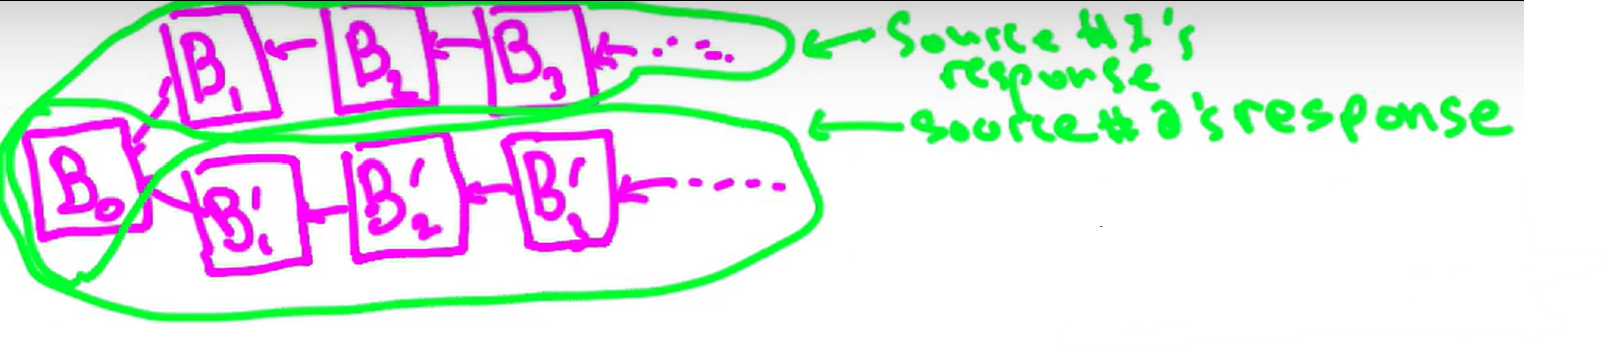
\includegraphics[scale = 0.5]{figures/f57.png}
    \caption{Long-range attack example}
    \label{fig:mesh1}
\end{figure}\\
\noindent
\textbf{Consequences of Long-Range Attacks:}
New nodes can't distinguish between legitimate blockchain and the attacker's alternative history.
Trust assumptions become more complex in PoS protocols due to the potential for long-range attacks.\\

\noindent
\textbf{Slashing Conditions in Proof-of-Stake (PoS):}\\
In PoS, slashing can occur for consistency violations.
Slashing requires on-chain evidence of double signing or other violations.
However, in a long-range attack scenario, branches may lack such on-chain evidence.\\

\noindent
\textbf{Tie-Breaking in Forked Chains:}\\
A natural thought might be to follow the longest chain, but this doesn't work.\\
\textbf{Costless Simulation Property:} In PoS protocols, stake reuse enables easy fabrication of alternative histories.\\
\textbf{Costless Simulation Property:} Unlike PoW, stake can be reused, allowing the creation of multiple alternative blockchains simultaneously.


\subsection{Cananical Long-Range Attack (Extreme Version)}
Let's explore the most extreme form of a long-range attack for better clarity, understanding that less extreme versions stem from the same underlying concepts. We'll use a proof-of-stake (PoS) blockchain protocol, such as a BFT-type protocol based on something like Tendermint. Assume this protocol has been running smoothly for a year, accumulating a year's worth of blocks without any forks or consistency issues.

\subsubsection{Initial Set of Stakers}
\begin{itemize}
    \item Focus on the initial set of stakers, where actual block production begins.
    \item These stakers have public keys and stake amounts locked in a staking contract.
    \item Let the public keys be denoted as $pk_1$ through $pk_n$.
\end{itemize}

\subsubsection{Assumptions}
\begin{itemize}
    \item At least two-thirds of the stake is controlled by honest nodes (or assume 100\% for simplicity).
    \item Over the year, these initial stakers have unstaked and cashed out their stakes.
    \begin{figure}[h]
    \centering
    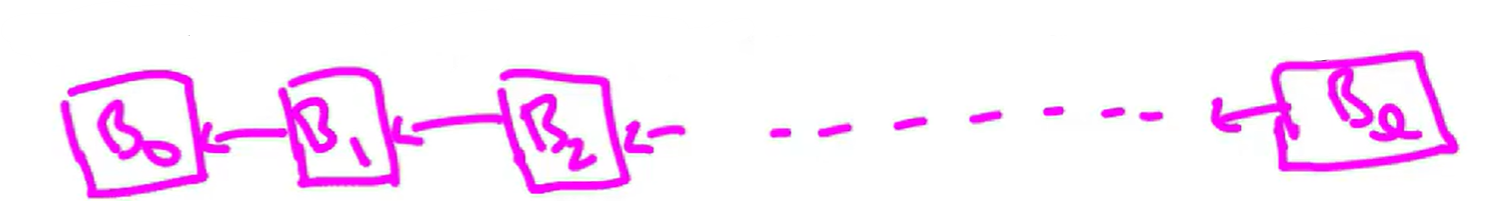
\includegraphics[scale = 0.5]{figures/f58.png}
    \caption{}
    \label{fig:mesh1}
    \end{figure}\\
\end{itemize}

\subsubsection{Attack Steps}
\begin{enumerate}
    \item \textbf{Acquiring Private Keys:}
    \begin{itemize}
        \item The attacker locates the owners of public keys $pk_1$ through $pk_n$.
        \item Since these owners have cashed out and unstaked, they no longer have assets tied to the blockchain protocol.
        \item The owners might be willing to sell their corresponding private keys, as they have no use for them anymore.
    \end{itemize}
    
    \item \textbf{Generating Alternative History:}
    \begin{itemize}
        \item The attacker now owns the private keys and can start creating an alternative blockchain history.
        \begin{figure}[h]
        \centering
        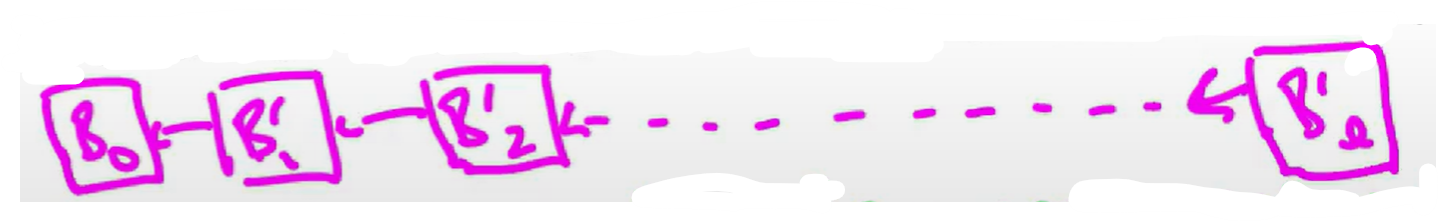
\includegraphics[scale = 0.5]{figures/f59.png}
        \caption{}
        \label{fig:mesh1}
        \end{figure}\\
        \item This alternative history can deviate significantly from the blocks produced by honest nodes over the past year.
    \end{itemize}
    
    \item \textbf{Rapidly Extending the Alternative History:}
    \begin{itemize}
        \item The attacker can quickly extend this alternative history using the reusability of stake.
        \item Unlike proof-of-work, where work done for one chain can't be reused for another, stake can be reused across different histories.
    \end{itemize}
\end{enumerate}

\subsubsection{Consequences}
\begin{itemize}
    \item New nodes cannot differentiate between the legitimate blockchain history and the attacker's alternative history.
    \item Trust assumptions become more intricate since PoS protocols rely on reusability of stake.
    \item The attack highlights the vulnerability of PoS protocols to long-range attacks due to the nature of stake reusability.
\end{itemize}

\subsubsection{Trust Assumptions for Newly Arriving Nodes}
\begin{itemize}
    \item A newly arriving node in a PoS protocol must make trust assumptions to correctly sync with the blockchain.
    \item These assumptions involve obtaining protocol software, Genesis block, learning the current state of the blockchain, and comparing information from multiple sources ($M$).
\end{itemize}

\subsubsection{Comparison to Proof-of-Work}
\begin{itemize}
    \item Long-range attacks are specific to PoS protocols and do not affect proof-of-work protocols like Nakamoto consensus.
    \item The difference lies in the reusability of stake versus the non-reusability of work.
\end{itemize}

\subsubsection{Stronger Trust Assumption for Consistency}
\begin{itemize}
    \item Long-range attacks reveal that the necessary condition for consistency in a PoS protocol is not sufficient.
    \item In addition to having at least two-thirds of stake controlled by honest nodes at any given moment, the same condition must hold for all future moments.
\end{itemize}


\section{Mitigations for Long-Range Attacks}
In the previous section, we discussed long-range attacks, their characteristics, and why they are specific to proof-of-stake protocols. Long-range attacks pose challenges and require stronger trust assumptions, especially when dealing with newly arriving nodes that want to sync up to the current state of a blockchain protocol.

\subsection*{Canonical Long-Range Attack and Extent of Concern}
A canonical long-range attack involves an attacker gaining control of old private keys, either by buying or stealing them. With this power, the attacker can quickly generate an alternative blockchain history using the costless nature of simulation.\\
The significance of long-range attacks is a topic of debate. Some consider them a significant threat, while others believe they can be managed through ad hoc methods. The true impact of long-range attacks in practice is still uncertain.
\subsection{Options for Addressing Long-Range Attacks}
Long-range attacks are distinct from proof-of-work protocols and pose challenges for trust assumptions, especially for newly arriving nodes aiming to sync with the current state of a blockchain protocol.\\
A canonical long-range attack can be summarized as follows: An attacker gains control over old private keys, either through purchase or theft. Utilizing this control and the costlessness of simulation, the attacker rapidly generates an alternative blockchain history. The significance of long-range attacks varies among experts, with differing opinions about their impact. Some find these attacks concerning, while others believe they can be managed using ad hoc methods. The practical implications of these attacks are not yet fully known, making it important to explore various options used or considered by different projects.

\subsubsection{Option 1: Continuous Online Monitoring}
The first option involves nodes continuously monitoring the blockchain's real-time creation. Nodes are assumed to be online from the protocol's inception and never go offline. While this assumption is effective in identifying alternative chains, it's impractical for permissionless blockchain protocols. By observing block production sequentially in real time, nodes can differentiate between the main chain and any latecomer chains.\\
However, this assumption is too strong for permissionless protocols and resembles a permissioned setting. This approach is not widely used in major proof-of-stake protocols.

\subsubsection{Option 2: Bounded Offline Periods}
Option 2 relaxes the continuous online assumption by allowing nodes to go offline temporarily, within a bounded period (denoted by $T$). This approach aims to strike a balance between accommodating node downtime and identifying alternative chains. Nodes are expected to return online within $T$ time steps.\\
Recalling from part 1, $T$ can be treated as the length of the cool-down period shown in the following timeline:\\
\begin{figure}[h]
    \centering
    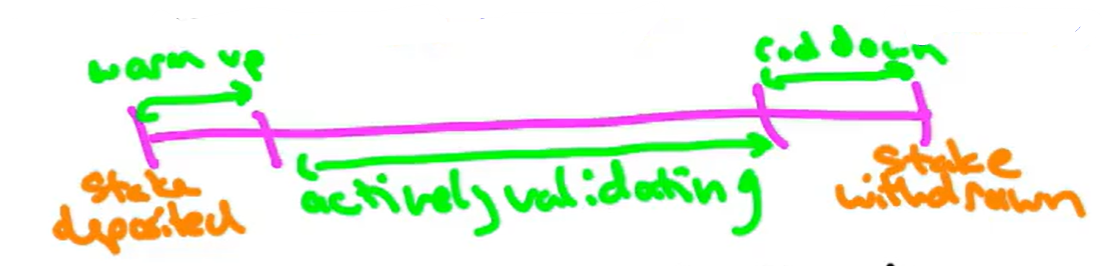
\includegraphics[scale = 0.5]{figures/f60.png}
    \caption{Timeline}
    \label{fig:mesh1}
\end{figure}\\
If a node goes offline for more than $T$ time steps, it's treated as a newly arriving node, and its trust in the blockchain's state is similar to the trust assumptions for newly arriving nodes.\\

Consider a scenario where node $i$ goes offline for a certain period of time $t$. During this time, new blocks continue to be added to the blockchain by other online nodes. Node $i$ eventually comes back online after $t$ time steps. In the absence of node $i$ during its offline period, it has no knowledge of the new blocks added to the blockchain. Therefore, when node $i$ reconnects, it needs to determine whether the blockchain it possesses (which ends at the last block it was aware of before going offline) is still part of the main chain.\\
To address this issue, node $i$ employs a strategy to reconcile its offline blockchain with the current state of the blockchain as observed by other nodes. Node $i$ initiates a process of information exchange with its peers once it regains connectivity. It requests information about the blockchain's evolution during its offline period from other nodes it can communicate with.\\
Upon receiving blockchain information from its peers, node $i$ carefully examines the structural characteristics of the blockchain during its offline period. It compares its own blockchain, which remained static during the downtime, with the evolving blockchain observed by other nodes. By analyzing the blockchain's structure, node $i$ can identify the common prefix between its offline blockchain and the current blockchain of the network.\\
Node $i$ then makes an informed decision based on the comparison. If the common prefix between its offline blockchain and the current blockchain is significant and recent, it indicates that the blockchain maintained its continuity during node $i$'s offline period. This implies that node $i$'s blockchain is still part of the main chain. On the other hand, if the common prefix is limited or outdated, it suggests that node $i$'s blockchain has diverged from the main chain, leading to a potential fork.\\
\begin{figure}[h]
    \centering
    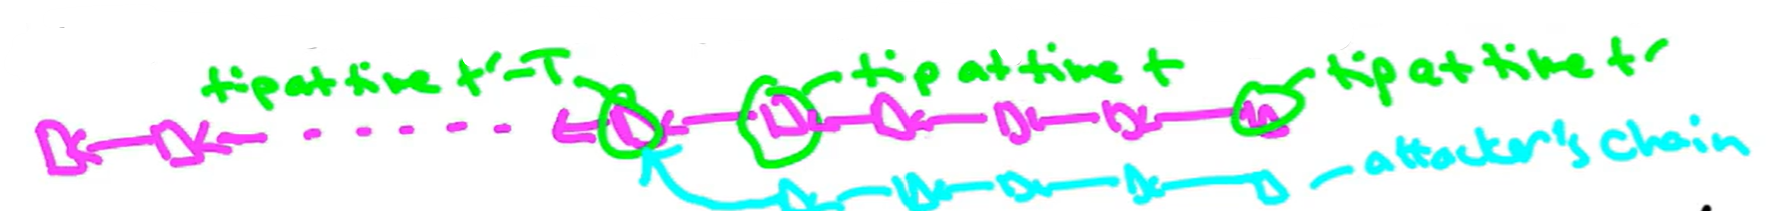
\includegraphics[scale = 0.5]{figures/f61.png}
    \caption{Example for Option 2}
    \label{fig:mesh1}
\end{figure}\\
This approach effectively enables nodes to tolerate temporary offline periods without compromising their ability to synchronize with the network and identify the main chain upon reconnection. The bounded offline period $T$ provides a reasonable timeframe within which nodes can be offline and still have a high likelihood of rejoining the main chain seamlessly.\\
Option 2 presents a pragmatic solution suitable for permissionless blockchain protocols, acknowledging that nodes may experience intermittent periods of online and offline states. By incorporating bounded offline periods and utilizing blockchain structure analysis, this option ensures the robustness of the blockchain network while accommodating the practical considerations of node connectivity.

\subsubsection{Option 3: Trusted Checkpoints}
Trusted checkpoints involve periodically finalizing blocks and treating them as trusted references. Nodes should disregard any chains that don't incorporate these trusted checkpoints. Checkpoints are akin to "phone-a-friend" solutions, where nodes rely on trusted information sources to determine the canonical chain.\\
Trusted checkpoints can be embedded in the protocol code or provided by trusted websites. While this approach simplifies trust assumptions, it's still centralized and can be vulnerable to attacks on the trusted source.

\subsubsection{Option 4: External Blockchain}
Option 4 suggests using an external blockchain, like Bitcoin, to periodically publish trusted checkpoints. This approach requires careful consideration of who can publish checkpoints and how to prevent fabricated information.

\subsubsection{Option 5: Proactive Defense}
Proactive defense aims to prevent long-range attacks by making old private keys useless. Cryptographic techniques, such as time-based key obsolescence, can ensure that keys lose value over time, reducing the effectiveness of attacks.

\subsubsection{Option 6: Verifiable Delay Functions (VDFs)}
Verifiable Delay Functions (VDFs) introduce computational delay into block validation. VDFs require solving time-consuming computations that cannot be easily parallelized. While not eliminating long-range attacks, VDFs increase the cost of simulation, making attacks more difficult and resource-intensive.\\
Current practice often relies on trusted checkpoints, while experimental approaches like VDFs and proactive defense are gaining attention. The best approach remains uncertain, and ongoing research will likely refine our understanding of long-range attacks and their mitigation.


\section{Proof-of-Stake vs. Proof-of-Work}
In permissionless consensus, Sybil resistance mechanisms are crucial to prevent nodes from gaining excessive power over the consensus protocol. Two dominant approaches are Proof-of-Work (PoW) and Proof-of-Stake (PoS). This section explores the advantages and disadvantages of these approaches.
\subsection{Energy Efficiency (Environmental Advantage)}
Proof-of-Work (PoW) protocols require nodes to continuously prove their hash rates, leading to significant energy consumption. This is due to the protocol's nature of allocating power to nodes based on the fraction of the overall hash rates they own. However, a fundamental issue arises from the unobservability of a node's hash rates by the protocol. In PoW, nodes must constantly demonstrate their hash rates to the protocol by running their computers and ASICs continuously. This process ensures that they maintain a certain likelihood of being selected as the next block proposer. Consequently, PoW protocols, such as Bitcoin, consume orders of magnitude more energy than traditional internet protocols.\\
This energy consumption has sparked debates about the environmental impact of PoW protocols like Bitcoin. While some argue that Bitcoin's unique position as a global, battle-tested permissionless payment system justifies its energy consumption, others express concerns about its energy use compared to other internet protocols. While opinions on the significance of this energy consumption vary, there is a consensus that PoW protocols consume more energy than is typical for internet protocols.\\
Proof-of-Stake (PoS) protocols, on the other hand, offer an alternative approach to achieving consensus without the same energy demands. In PoS protocols, a node's control over the protocol, such as its likelihood of being elected as a block proposer, is proportional to the stake it holds in a staking contract. This stake, denominated in the blockchain protocol's native currency, is directly observable to the protocol. Unlike PoW, where hash rates are unobservable and require constant proving, PoS protocols automatically know the amount of stake each node has locked up.\\
As a result, PoS blockchain protocols exhibit energy consumption levels comparable to those of other internet protocols. This is a significant departure from the energy-intensive nature of PoW protocols like Bitcoin. The shift towards PoS protocols in recent years is partly driven by the desire to reduce energy consumption while maintaining the security and integrity of the blockchain.\\
While proponents of PoW protocols may argue that Bitcoin's unique position justifies its energy use, and some energy consumption comes from renewable sources, the consensus remains that PoS protocols provide a more energy-efficient alternative.

\subsection{Latency and Finality (Performance Advantage)}
Latency and finality are critical aspects of consensus protocols that directly impact the efficiency and reliability of blockchain systems. In this section, we'll delve deeper into how Proof-of-Stake (PoS) protocols offer significant improvements in terms of latency and finality compared to the traditional Proof-of-Work (PoW) protocols.
\subsubsection{Latency}
Latency refers to the time that elapses between when a transaction is submitted to the blockchain protocol and when it is confirmed and considered finalized in a block. The design of PoW protocols, specifically Nakamoto consensus, introduces inherent latency due to the nature of the longest chain consensus mechanism.\\
In Nakamoto consensus, a security parameter $K$ determines how deep a block needs to be in the longest chain to be considered sufficiently finalized. Only blocks beyond this depth are deemed confirmed. As a result, transactions may need to wait for multiple blocks to be added on top of them before achieving confirmation. This leads to latency that can range from minutes to hours, depending on the specific implementation.\\
On the other hand, PoS protocols, especially when combined with Byzantine Fault Tolerance (BFT), offer significant improvements in latency. With the integration of a BFT consensus mechanism like Tendermint, PoS protocols can achieve faster finality by considering a block as finalized as soon as it obtains a stage two Quorum certificate. This allows for near-immediate confirmation of transactions, drastically reducing latency compared to PoW-based systems.

\subsubsection{Finality}
Finality is the assurance that a transaction or block will not be reversed or altered in the future. In Nakamoto consensus, finality is probabilistic even for well-behaved networks, and it becomes even more uncertain in the presence of network outages or attacks. This probabilistic nature stems from the potential for an alternative chain to emerge and invalidate previously confirmed blocks.\\
PoS protocols, particularly those incorporating BFT mechanisms, offer stronger finality guarantees. Once a block receives a stage two Quorum certificate in a PoS-BFT system, it is considered irrevocably finalized. This means that the block is immune to chain reorganizations or adversarial behavior, providing a high degree of transaction certainty.\\
To illustrate this point, consider the scenario in which a double spend attack occurs. In a PoW protocol, the uncertainty of finality allows for the possibility of an attacker reverting confirmed transactions. However, in a PoS-BFT protocol like Tendermint, the finality achieved through stage two Quorum certificates ensures that transactions are secure against such attacks.

\subsection{Security and Slashing (Security Advantage)}
One significant advantage of Proof-of-Stake (PoS) protocols is the potential for using slashing mechanisms, which enhances the security of the blockchain network. Slashing provides a means to discourage malicious behavior and enables the recovery from certain types of attacks, such as the infamous 51\% attack.\\
In a PoS protocol, nodes gain influence in the consensus protocol based on the amount of stake they hold in staking contracts. This stake is a directly observable resource, allowing the protocol to have accurate information about each node's influence. This is in stark contrast to Proof-of-Work (PoW) protocols, where hash rate is the key resource, but its unobservability by the protocol creates challenges in detecting malicious activity.\\

Consider the scenario of a 51\% attack, where an adversary captures a significant portion of the network's resources. In PoW protocols, options are limited. One approach could involve a hard fork that changes the cryptographic hash function, rendering the attacker's specialized hardware useless. However, this also affects honest nodes, leading to collateral damage.\\

In contrast, PoS protocols offer a more surgical approach through slashing. Slashing involves programmatically penalizing nodes that deviate from honest behavior. This is possible because the stake held by nodes is observable. For instance, in Tendermint, a PoS protocol, a double spend attack requires conflicting blocks to be finalized at the same block height, indicating malicious behavior. By slashing the stake of nodes that voted on conflicting blocks, the protocol can confiscate their economically valuable resources.\\
Furthermore, the implementation of slashing can take different forms, such as a hard fork or programmatic slashing. Hard forks require coordination among stakeholders to upgrade the protocol. Programmatic slashing, on the other hand, allows the protocol to automatically enforce penalties based on the evidence present in the blockchain itself. This enables the network to react swiftly to security threats without requiring a full-scale protocol upgrade.\\
While programmatic slashing presents a promising option for recovering from attacks, its usage and best practices vary among PoS protocols. Ethereum's post-merge design, for instance, incorporates programmatic slashing to enhance security.\\
In contrast, PoW protocols lack a comparable mechanism for targeted penalties. The inability to slash malicious actors' resources programmatically or surgically hampers their ability to recover from attacks. PoS protocols thus provide a security advantage by offering the option of slashing, which contributes to a more robust defense against adversarial actions.\\
This security advantage is another compelling reason behind the growing adoption of PoS protocols in the blockchain ecosystem, as it provides a more fine-tuned and proactive approach to addressing security threats and maintaining network integrity.

\subsection{Debates and Common Confusion}
The debate over Proof-of-Work (PoW) versus Proof-of-Stake (PoS) encompasses several key points of contention and areas of common confusion. By addressing these aspects, we can better understand the nuanced considerations surrounding these consensus mechanisms.

\subsubsection{Benefits of PoS vs. Costs}
One major point of debate revolves around whether the benefits of PoS outweigh its associated costs. While both PoW and PoS offer distinct advantages, such as energy efficiency and reduced latency in PoS, critics argue that PoS may introduce security vulnerabilities due to its reliance on stake ownership. Proponents of PoS emphasize its potential to achieve similar security while consuming less energy and enabling faster transactions. Assessing which benefits are more valuable and whether potential drawbacks are manageable remains a central issue of discussion.

\subsubsection{Misleading Discourse}
Common misconceptions and misleading arguments often cloud discussions about PoW and PoS. One prominent example is the conflation of a methodology (PoW or PoS) with a specific protocol that implements it. It's essential to distinguish between the broader approach and the particular implementations, as each protocol can have unique features and trade-offs.\\
Another source of confusion stems from comparing apples to oranges, such as comparing PoW protocols like Bitcoin to everyday internet protocols. While PoW may consume significant energy, its role as a global, battle-tested payment system introduces complexity when evaluating its environmental impact. Comparing it to simpler internet protocols might oversimplify the discussion.\\
Furthermore, the notion of "energy use" itself can be misleading. The impact of PoW energy consumption depends on factors like the energy source's sustainability and the overall energy market dynamics. Failing to consider these factors can lead to skewed conclusions about the ecological implications of PoW.

\subsection{Disadvantages of Proof-of-Stake}
Now, we'll get into the disadvantages of Proof-of-Stake (PoS) blockchain protocols. While some drawbacks are more forgivable in the context of Proof-of-Work (PoW), PoS protocols have their unique challenges and trade-offs. Let's examine these disadvantages and their implications.

\subsubsection{Complexity and Complications}
One of the initial drawbacks of PoS blockchain protocols is their inherent complexity. While not a fundamental theorem, an observation of the current landscape shows that PoS protocols tend to be more intricate than their PoW counterparts. This complexity is reflected in various aspects, including protocol design and implementation. For example, Ethereum's transition from PoW to PoS took years of development and testing before achieving consensus. The additional intricacy introduces a higher probability of design flaws and implementation bugs. Even seemingly simple distributed protocols can be challenging to implement correctly, and more complex protocols amplify this risk.\\
The argument against excessive complexity is rooted in the idea that intricate protocols are harder to get right, increasing the risk of undetected vulnerabilities. While complexity can lead to innovative functionality, it also requires more effort and expertise to ensure robustness and security.

\subsubsection{Expanded Attack Vectors}
The complexity of PoS protocols contributes to a second disadvantage: the emergence of new attack vectors. Although not a proven theorem, this observation holds true in practice. PoS blockchain protocols are susceptible to a broader range of attacks compared to PoW protocols. This vulnerability is partially due to the property of costless simulation inherent in PoS systems.\\
Costless simulation enables nodes in a PoS protocol to quickly fabricate alternative histories at a low cost. While this attribute enables certain functionalities, such as long-range attacks, it introduces security challenges. For instance, the long-range attack utilizes costless simulation to generate a fabricated history using stolen or purchased old keys. In contrast, PoW protocols require costly simulation, making such attacks significantly more difficult.\\
This expanded set of attack vectors increases the risk profile of PoS protocols and demands advanced security measures and careful protocol design to mitigate these threats effectively.

\subsubsection{Stronger Trust Assumptions}
A final fundamental disadvantage of PoS protocols lies in their need for stronger trust assumptions compared to PoW protocols. This need arises due to the lack of a clear objective criterion for selecting the valid chain among competing chains, a criterion that PoW protocols possess through accumulated work.\\
In PoW protocols, new nodes can determine the valid chain based on the amount of work devoted to each chain. PoS protocols lack a similarly objective criterion, leading to the requirement for stronger trust assumptions. These assumptions involve additional mechanisms like trusted checkpoints or external sources for validation, further complicating the consensus process and introducing the potential for centralization.\\
While PoS proponents might argue that these stronger trust assumptions are manageable, they do introduce an element of uncertainty, especially when compared to the relative simplicity of the Nakamoto consensus mechanism in PoW.

\subsubsection{Assessment and Future Outlook}
These three disadvantages—complexity, expanded attack vectors, and stronger trust assumptions—form the core challenges of PoS blockchain protocols. While proponents of PoS acknowledge these drawbacks, they argue that ongoing advancements in protocol design, testing, and real-world experience will progressively address and mitigate these concerns. The intricate nature of PoS protocols, combined with the evolving security landscape, calls for careful consideration and continuous improvement as the technology matures.\\

Now we will discuss two controversial questions:\\
\begin{enumerate}
    \item Which of PoW or PoS is "more permissionless"?
    \item Which of PoW or PoS is "more decentralized"?
\end{enumerate}
\subsection{Permissionlessness in PoS and PoW}
The concept of \textit{permissionlessness} is a key feature in blockchain protocols, often debated when comparing PoW and PoS. This term refers to the degree of openness and accessibility for individuals to participate in the consensus process and interact with the blockchain network.

\subsubsection{Proof-of-Work (PoW)}
In the context of PoW protocols, permissionlessness is achieved through a specific mechanism. When a participant attempts to mine a new block, the protocol treats them as an anonymous entity until they successfully solve a cryptographic puzzle and present a block to the network. Only at this point does the protocol become aware of the participant's existence and their associated public key. Notably, the inclusion of the public key in the block, which is used to claim the block reward, is optional. This anonymity and lack of prior registration can be seen as a form of permissionlessness.\\
However, it's important to note that this concept of permissionlessness in PoW is focused on the act of contributing to block production. It doesn't necessarily imply that the entire network or ecosystem is completely open and free from certain requirements, as aspects such as accessing and using the cryptocurrency associated with the blockchain might involve exchanges or wallets that require user identification.

\subsubsection{Proof-of-Stake (PoS)}
In PoS protocols, permissionlessness operates differently due to the staking mechanism. To participate in consensus and contribute to block creation, a user is required to create a staking contract by locking a certain amount of the native cryptocurrency into it. This contract is associated with the user's public key, which is used for signing blocks or votes in the consensus process. This means that the protocol, as well as anyone observing the staking contract, is aware of the participant's public key before they even begin producing blocks.\\
This registration-like requirement in PoS protocols may appear to introduce a mild form of permission, as users need to establish their identity (in the form of a public key) before actively participating in consensus. However, it's important to emphasize that this registration is limited to the public key and doesn't involve revealing additional personal information. Furthermore, the registration process is relatively straightforward and doesn't involve complex verification procedures.

\subsubsection{Comparing Permissionlessness}
When comparing the permissionlessness of PoW and PoS, it's important to consider the specific context in which it applies. While PoW might offer a certain level of anonymity until a participant mines a block, PoS requires a minimal form of registration before contributing to consensus. However, the distinction between the two is not necessarily drastic, as both mechanisms allow individuals to engage with the blockchain network without extensive prerequisites.

\subsection{Decentralization Considerations}

The concept of \textit{decentralization} is a highly debated topic in the realm of blockchain protocols. However, the definition of decentralization can vary significantly depending on the context and the specific aspects being considered. It is crucial to explore the different interpretations of decentralization before attempting to compare Proof-of-Work (PoW) and Proof-of-Stake (PoS) protocols.

\subsubsection{Minimum Computing Requirements as a Measure of Decentralization}

One common approach to assessing decentralization involves evaluating the minimum computing power necessary to verify the correctness of a blockchain's progression. In this context, "verifying correctness" refers to the ability of a node to monitor the blockchain's transactions and blocks without actively participating in the block production process. It's important to note that this definition of decentralization focuses solely on the computational resources required for this passive verification.\\

\noindent
\textbf{Bitcoin's Example of Minimal Computing Requirements}\\
A well-known example in this context is Bitcoin, which is often praised for its decentralized nature concerning minimum computing requirements. The reason for Bitcoin's favorable score in this metric is not tied to its Proof-of-Work consensus mechanism; rather, it results from specific design choices.\\
Bitcoin utilizes the longest chain consensus mechanism, which is relatively lightweight compared to more complex Byzantine Fault Tolerant (BFT) protocols. This choice allows nodes to efficiently verify the correctness of the blockchain's progression without demanding significant computational resources. Additionally, Bitcoin's parameter choices, such as the relatively slow block rate (averaging one block every 10 minutes) and block size, contribute to reducing the computational burden on network participants.\\
In essence, the decentralized nature of Bitcoin concerning minimal computing requirements is a result of its consensus mechanism and parameter settings. This underscores the point that this form of decentralization is not inherently tied to the choice between PoW and PoS but rather to specific protocol design considerations.

\subsubsection{Distribution of Cryptocurrency}
One interpretation of decentralization pertains to the evenness of the distribution of the cryptocurrency within the blockchain protocol. This concept involves ensuring that the cryptocurrency is distributed fairly among participants, although this notion presents challenges that require thorough consideration.\\

\noindent
\textbf{Evolution of Proof-of-Stake Protocols:} Currently, there is limited historical data available to fully observe the evolution of Proof-of-Stake (PoS) blockchain protocols. Most major PoS protocols have only been in existence for a relatively short period. This limitation makes it difficult to draw definitive conclusions about whether there are systematic differences in the distribution of cryptocurrency between Proof-of-Work (PoW) and PoS protocols.\\

\noindent
\textbf{Wealth Concentration and Pareto Distribution:} A crucial aspect to recognize is that aiming for a perfectly even distribution of cryptocurrencies might not be a realistic goal. The phenomenon of wealth concentration is a natural occurrence, and the Pareto distribution, which is commonly observed in income distributions across societies, suggests that wealth tends to naturally concentrate.\\
While it is aspirational to utilize blockchain and cryptocurrencies for achieving fair income distribution, it is important to acknowledge that wealth concentration is a powerful force that tends to persist. It is unrealistic to expect cryptocurrencies to achieve a more even distribution than the fiat currencies of modern democracies.\\

\noindent
\textbf{Decentralization Through Initial Distribution:} Achieving a fair initial distribution of a new cryptocurrency is a critical consideration. While Bitcoin notably launched with an all-zero initial distribution, where no Bitcoins were in existence at the protocol's launch, replicating this approach for other projects might not be feasible. Implementing a non-zero initial distribution could be a practical strategy to generate interest and support for a new blockchain protocol.\\
Projects should aim to establish a reasonably fair initial distribution by involving a diverse set of stakeholders. This can be achieved through methods such as airdrops, where new cryptocurrency is distributed to various addresses. Airdrops aim to create a broad base of holders who have a stake in the protocol's success.\\

\noindent
\textbf{Challenges with Airdrops:} Executing effective airdrops presents challenges, particularly concerning Sybil attacks, where a single entity controls multiple addresses to receive more rewards. Crafting airdrop strategies to prevent such attacks and ensure equitable distribution is an ongoing area of research and development.

\subsubsection{Distribution of Control Over the Protocol}
Decentralization also encompasses the distribution of control over the blockchain protocol itself. This aspect examines how the authority to make decisions and influence protocol changes is distributed among participants.

\noindent
\textbf{Mining Pools and Hash Rate Concentration:} In Proof-of-Work (PoW) protocols, the distribution of control is often measured by the concentration of hash rate among mining pools. Hash rate refers to the computational power contributed by miners to secure the network and validate transactions.\\
A notable observation in PoW protocols, such as Bitcoin, is the presence of large mining pools. These mining pools consist of multiple individual miners who combine their hash power to increase the chances of mining a block and receiving rewards. The concentration of hash rate in a few major mining pools has raised concerns about centralization.\\
For instance, some mining pools can collectively control a significant portion of the total hash rate dedicated to the protocol. This concentration potentially grants these pools substantial influence over protocol decisions, including updates, forks, and validation of transactions. Economies of scale and efficient infrastructure, like advanced cooling systems, allow larger mining operations to dominate the network.

\noindent
\textbf{Staking Pools and Protocol Control:} Proof-of-Stake (PoS) protocols introduce a similar concept with staking pools, which affects the distribution of control over the protocol. Staking involves participants locking up a certain amount of cryptocurrency as collateral to validate transactions and secure the network.\\
In PoS protocols like Ethereum, participants have the option to delegate their stake to staking pools. These pools act as service providers, handling the technical requirements of running a validating node. By delegating their stake to a pool, participants can earn staking rewards without directly managing a node. This delegation mechanism has the potential to influence protocol control.\\
The question arises: Does the concentration of stake within staking pools lead to centralization of control over the protocol? Just as with mining pools in PoW, the distribution of control in PoS can be impacted by the size and influence of staking pools.\\
However, determining the impact of staking pools on protocol control is complex and subject to interpretation. It's not clear whether a single large staking pool should be considered as a single powerful entity or as a collection of individual participants who have chosen to delegate their stake. This uncertainty complicates the assessment of control distribution within PoS protocols.

\subsubsection{Complexity of Decentralization}
In summary, the concept of decentralization in blockchain protocols is intricate and multifaceted, involving various interpretations and considerations. The meaning of decentralization can differ among individuals, leading to diverse viewpoints on what it truly entails. As we have seen, there are competing definitions of decentralization, making it challenging to reach a consensus on its precise significance.\\
Furthermore, determining the practical relevance of different aspects of decentralization remains an ongoing challenge. While decentralization is a central tenet of blockchain technology, its real-world implications can be complex and multifaceted.\\
When comparing Proof-of-Work (PoW) and Proof-of-Stake (PoS) protocols, the question of which approach better achieves decentralization is not straightforward. Each approach has its advantages and disadvantages in terms of decentralization criteria, making it difficult to declare a definitive winner.\\
For instance, PoS protocols offer benefits like reduced energy consumption, improved latency, and finality guarantees. These advantages contribute to decentralization in certain respects, as they address some of the limitations associated with PoW. However, PoS protocols also introduce complexities, such as additional attack vectors and stronger trust assumptions, which can impact decentralization efforts.\\
On the other hand, PoW protocols, exemplified by Bitcoin, have demonstrated a significant degree of decentralization over the years. However, they too face challenges related to hash rate concentration in large mining pools. While mining pools help ensure more regular rewards for participants, they also raise concerns about centralization of control.\\
The complexity deepens when considering the distribution of cryptocurrency and control over the protocol. Achieving a fair initial distribution of a new cryptocurrency is a crucial goal for both PoW and PoS protocols. Strategies like airdrops aim to involve a wide range of stakeholders, but challenges such as Sybil attacks must be addressed.\\
Additionally, the evolution of currency distribution over time presents a unique set of challenges. Protocol design can impact the concentration of wealth and influence income inequality. Whether PoS protocols lead to the rich getting richer is a common misconception; staking rewards are based on proportional stakes, and while larger stakes earn higher rewards in absolute terms, the distribution remains unchanged if everyone receives their fair share.\\
The emergence of mining pools in PoW and staking pools or delegation services in PoS introduces further complexity to the decentralization landscape. While these mechanisms allow broader participation and more predictable rewards, questions arise about their impact on protocol control and centralization.\\
In conclusion, the complexity of decentralization arises from the interplay of various factors, including differing interpretations of the concept, the nuanced comparison between PoW and PoS protocols, and the challenges associated with cryptocurrency distribution and protocol control. As the blockchain ecosystem continues to evolve, debates about permissionless and decentralized systems will persist, requiring careful consideration of these intricacies when assessing consensus mechanisms.\\
By navigating through this complex terrain, you have gained a deep understanding of the intricacies of decentralization in blockchain protocols. This knowledge positions you to engage in informed discussions and contribute meaningfully to the ongoing exploration of blockchain technology.